\documentclass[11pt,a4paper]{article}

\usepackage[T1]{fontenc}
\usepackage{mathpazo}
\usepackage[scaled=0.92]{helvet}
\usepackage[margin=1in]{geometry}
\usepackage{microtype}
\usepackage{amsmath,amssymb}
\usepackage{graphicx}
\usepackage{pgf}
\usepackage{booktabs}
\usepackage{xcolor}
\usepackage[numbers,sort&compress]{natbib}
\usepackage{caption}
\usepackage[hidelinks]{hyperref}
\usepackage{enumitem}
\graphicspath{{figures/}}
\usepackage{placeins}
\renewcommand{\topfraction}{0.85}
\renewcommand{\textfraction}{0.1}
\renewcommand{\floatpagefraction}{0.75}

\definecolor{qink}{HTML}{1D1F52}
\captionsetup{font=small,labelfont=bf,margin=0.5em}
\setlist{itemsep=2pt,topsep=4pt}
\renewcommand{\sectionmark}[1]{}
\newcommand{\figwidth}{\linewidth}
\newcommand{\ket}[1]{\lvert #1\rangle}
\newcommand{\expect}[1]{\langle #1\rangle}

\title{\sffamily\bfseries\color{qink}One Tile, Two True Colors:\\[2pt]
  \large\mdseries Quantum Contextuality as a Design Material}
\author{Lakshmi Monish\\[2pt]
  \small\url{https://github.com/QubitMan-hub/Qontext}}
\date{October 2026}

\begin{document}
\maketitle

\begin{abstract}
\noindent Design systems assume that a token has one value. A brand color is one color wherever it appears. Quantum
mechanics has a family of results, the Kochen-Specker theorem and one of its simplest forms, the Mermin-Peres square,
which say that some quantities cannot be given one value that holds whatever else is measured with them. We use that
result as a design material. In Qontext, each of the nine tiles of the Mermin-Peres square holds two colors: one when
it is read with its row and one when it is read with its column. Hue is treated as quantum phase, so the colors come
from an even harmony on the OKLCH wheel, and every reading obeys the square's six product rules. No fixed table of
colors can do this. An exhaustive search over all 512 tables confirms that at most five of the six rules can hold. We
show that the two readings always differ on an odd number of tiles, and that the expected number is between 3 and 4
for any pure two-qubit state. We describe the engine, a contrast checker that tests text against every color a tile
can take, a theme dial built from the interferometer model, and a case study in which the nine panels of a sneaker
are the nine tiles and the two feet are the two readings. Everything runs as exact simulation in a web browser. We
say plainly what this is and is not: the system is small enough to simulate on a phone, and we claim no quantum
advantage.
\end{abstract}

\section{Introduction}

A design token is a named value: \texttt{color-accent} is \texttt{\#3fc0f2}, everywhere, for everyone. Modern design
systems do let tokens change with context. A token can have a light mode and a dark mode, or a hover state. But in
every case a designer picks the value for each context by hand, and nothing stops them from picking one value for all
of them. The context is a label.

Quantum mechanics offers a different kind of context. In 1967 Kochen and Specker showed that there are sets of
measurements whose outcomes cannot all be fixed in advance, independent of which other compatible measurements are
made alongside them \citep{kochen1967,bell1966}. In 1990 Peres and Mermin found a version small enough to write on a
napkin: a three by three grid of two-qubit observables, now called the Mermin-Peres square
\citep{peres1990,mermin1990}. Each row and each column is a set of observables that can be measured together, and
quantum mechanics fixes the product of their outcomes. No assignment of $+1$ and $-1$ to the nine cells can satisfy
all six products at once. So a cell's value depends on whether it was measured with its row or with its column.

Qontext turns this into color. Each cell becomes a tile. Each outcome becomes a hue: $+1$ shows the tile's harmony
color, $-1$ its complement. Reading the grid by rows gives one coloring, reading it by columns gives another, and the
mathematics guarantees that the two can never be the same coloring. The context is no longer a label. It is a
constraint that no fixed palette can meet.

We built this as a working product, not a demonstration: a website where every visitor gets their own measured
palette, a studio for designers (the Atelier), a 12\,KB runtime that applies a measured palette to any website, a
Figma plugin with Row and Column variable modes, and a command line tool that runs the same circuits on IBM Quantum
hardware. This paper describes the ideas and their limits. Its contributions are:
\begin{itemize}
  \item A mapping from the Mermin-Peres square to color tokens, with hue as quantum phase (Section~\ref{sec:method}).
  \item Two short results about the two readings: they differ on an odd number of tiles, and on $\tfrac12\sum_t
        (1-\expect{O_t}^2)$ tiles on average, which is between 3 and 4 for any pure state (Section~\ref{sec:two}).
  \item Bouncer, a contrast check over every color a tile can take, and the Phase Dial, a light and dark theme
        built as an interferometer (Section~\ref{sec:usable}).
  \item Pair Production, a worked case of an artist designing a sneaker drop with the system
        (Section~\ref{sec:pair}).
  \item An implementation in which every classical limit shown to the user is checked by exhaustive search in the
        test suite (Section~\ref{sec:impl}).
\end{itemize}
We are careful about one point throughout. Two qubits are easy to simulate, so nothing here needs a quantum computer.
What the physics gives is a grammar for color that comes with a proof (Section~\ref{sec:limits}).

\section{Background}
\label{sec:background}

\paragraph{Contextuality.} Two observables are compatible when they commute, so they can be measured together. A
\emph{context} is a set of mutually compatible observables. A noncontextual hidden variable model gives every
observable one predetermined value, the same in every context it appears in. The Kochen-Specker theorem says no such
model can reproduce quantum mechanics in dimension three or more \citep{kochen1967}. A recent review covers the
theory and the experiments in depth \citep{budroni2022}.

\paragraph{The Mermin-Peres square.} Table~\ref{tab:square} shows the version we use. $X_i$, $Y_i$ and $Z_i$ are
Pauli operators on qubit $i$. The three observables in each row commute, and so do the three in each column. Each row
multiplies to the identity, as do the first two columns. The third column multiplies to minus the identity, because
$X_1X_2 \cdot Z_1Z_2 = -Y_1Y_2$. Our engine derives these six signs from the matrices when it loads, rather than
storing them.

\begin{table}[h]
\centering
\small
\begin{tabular}{c|ccc|c}
\toprule
 & column 1 & column 2 & column 3 & row product \\
\midrule
row 1 & $X_1$ & $X_2$ & $X_1X_2$ & $+I$ \\
row 2 & $Z_2$ & $Z_1$ & $Z_1Z_2$ & $+I$ \\
row 3 & $X_1Z_2$ & $Z_1X_2$ & $Y_1Y_2$ & $+I$ \\
\midrule
column product & $+I$ & $+I$ & $-I$ & \\
\bottomrule
\end{tabular}
\caption{The Mermin-Peres square as Qontext uses it. Rows and columns are the six contexts.}
\label{tab:square}
\end{table}

Suppose each cell had a fixed value $v_t \in \{+1,-1\}$. Multiplying all nine values row by row gives $+1$, since
each row gives $+1$. Multiplying them column by column gives $-1$. It is the same nine numbers, so this is a
contradiction, and at least one of the six rules must fail. Checking all $2^9 = 512$ tables confirms that the best
any table can do is five rules out of six. Quantum mechanics satisfies all six on every run, whatever the state, which
makes the square a state-independent test. It has been measured with trapped ions \citep{kirchmair2009}, on IBM's
public quantum computers \citep{dikme2020}, and as a two-player game with entangled photons \citep{xu2022}.

\paragraph{Other structures.} The engine also builds the KCBS pentagram \citep{kcbs2008}, the CHSH setting
\citep{chsh1969,tsirelson1980}, and three Kochen-Specker sets: Peres's 33 rays \citep{peres1991}, the 18 vectors of
Cabello, Estebaranz and Garc\'ia-Alcaine \citep{cabello1996}, and the 13 rays of Yu and Oh \citep{yuoh2012}.
Table~\ref{tab:limits} lists the classical and quantum values the interface shows. Each classical value in the table
is checked by exhaustive search in the test suite, not copied from the literature.

\begin{table}[h]
\centering
\small
\begin{tabular}{lccc}
\toprule
Structure & classical limit & quantum value & search in the tests \\
\midrule
Mermin-Peres score (rules held, as $2k-6$) & 4 & 6 & all 512 tables \\
KCBS sum of probabilities & 2 & $\sqrt5 \approx 2.236$ & all 32 assignments \\
CHSH value $S$ & 2 & $2\sqrt2 \approx 2.828$ & all 16 strategies \\
Yu-Oh expression & 8 & $25/3 \approx 8.33$ & all 8{,}192 assignments \\
Peres 33, Cabello 18 coloring & impossible & & complete search \\
\bottomrule
\end{tabular}
\caption{Classical limits and quantum values shown in Qontext. The Yu-Oh set can be colored, but its expression still
separates the two.}
\label{tab:limits}
\end{table}

\section{From observables to colors}
\label{sec:method}

\paragraph{Hue as phase.} A quantum system with $d$ levels has a clock operator whose eigenvalues are the $d$-th roots
of unity, $\omega^k = e^{2\pi i k/d}$. They sit evenly on a circle. We place them on the hue circle of OKLCH, the
cylindrical form of the Oklab color space \citep{ottosson2020,csscolor4}, so a palette with base hue $h_0$ has the
hues
\begin{equation}
  h_k = h_0 + \frac{360^\circ k}{d}, \qquad k = 0, \dots, d-1,
\end{equation}
all at one lightness $L$ and chroma $C$. With $d=2$ this is a complementary pair, with $d=3$ a triad, with $d=4$ a
square, up to $d=8$. These are the classic even harmonies of color theory \citep{itten1961}. The analogy is
structural: the eye does not see quantum phase, but the same arithmetic of turning by equal steps produces both.

\paragraph{Tile colors.} Tile $(r,c)$, with $r,c \in \{0,1,2\}$, takes harmony color $k = (3r+c) \bmod d$. An outcome
of $+1$ shows hue $h_k$. An outcome of $-1$ shows $h_k + 180^\circ$, its complement. A three by three grid therefore
has eighteen tile colors, two per tile, drawn from at most $2d$ distinct hues.

\paragraph{Measurement.} The engine samples outcomes exactly. For a context with observables $A$ and $B$ and third
observable $C = sAB$ (with $s = \pm1$ from Table~\ref{tab:square}), the probability of outcomes $(a,b)$ on state
$\ket\psi$ is
\begin{equation}
  P(a,b) = \Bigl\lVert \tfrac{I+aA}{2}\,\tfrac{I+bB}{2}\ket\psi \Bigr\rVert^2, \qquad c = s\,a\,b .
\end{equation}
Each of the six contexts is measured on its own copy of $\ket\psi$, as in the experiments above. The random numbers
come from a seeded generator, so a measurement is reproducible from two numbers: the state's seed and the
measurement's seed. On the website each visitor gets a measurement seed between 1 and 9{,}999{,}999, called their
\emph{world}, and the whole site is colored from it. The state is a fixed random two-qubit state (Gaussian
amplitudes, normalized). A design, with its harmony, lightness, chroma and seeds, travels as a short code beginning
\texttt{QX1.} that any part of the system can open.

\section{Two true colors}
\label{sec:two}

Reading the grid by rows takes each tile's value from its row's measurement. Reading it by columns takes each tile's
value from its column's measurement. Figure~\ref{fig:grid} shows both readings for one world. Three tiles differ.

\begin{figure}[t]
  \centering
  \resizebox{\figwidth}{!}{%% Creator: Matplotlib, PGF backend
%%
%% To include the figure in your LaTeX document, write
%%   \input{<filename>.pgf}
%%
%% Make sure the required packages are loaded in your preamble
%%   \usepackage{pgf}
%%
%% Also ensure that all the required font packages are loaded; for instance,
%% the lmodern package is sometimes necessary when using math font.
%%   \usepackage{lmodern}
%%
%% Figures using additional raster images can only be included by \input if
%% they are in the same directory as the main LaTeX file. For loading figures
%% from other directories you can use the `import` package
%%   \usepackage{import}
%%
%% and then include the figures with
%%   \import{<path to file>}{<filename>.pgf}
%%
%% Matplotlib used the following preamble
%%   \def\mathdefault#1{#1}
%%   \everymath=\expandafter{\the\everymath\displaystyle}
%%   \IfFileExists{scrextend.sty}{
%%     \usepackage[fontsize=9.000000pt]{scrextend}
%%   }{
%%     \renewcommand{\normalsize}{\fontsize{9.000000}{10.800000}\selectfont}
%%     \normalsize
%%   }
%%   \usepackage{mathpazo}
%%   \makeatletter\@ifpackageloaded{underscore}{}{\usepackage[strings]{underscore}}\makeatother
%%
\begingroup%
\makeatletter%
\begin{pgfpicture}%
\pgfpathrectangle{\pgfpointorigin}{\pgfqpoint{6.300000in}{2.350000in}}%
\pgfusepath{use as bounding box, clip}%
\begin{pgfscope}%
\pgfsetbuttcap%
\pgfsetmiterjoin%
\definecolor{currentfill}{rgb}{1.000000,1.000000,1.000000}%
\pgfsetfillcolor{currentfill}%
\pgfsetlinewidth{0.000000pt}%
\definecolor{currentstroke}{rgb}{1.000000,1.000000,1.000000}%
\pgfsetstrokecolor{currentstroke}%
\pgfsetdash{}{0pt}%
\pgfpathmoveto{\pgfqpoint{0.000000in}{0.000000in}}%
\pgfpathlineto{\pgfqpoint{6.300000in}{0.000000in}}%
\pgfpathlineto{\pgfqpoint{6.300000in}{2.350000in}}%
\pgfpathlineto{\pgfqpoint{0.000000in}{2.350000in}}%
\pgfpathlineto{\pgfqpoint{0.000000in}{0.000000in}}%
\pgfpathclose%
\pgfusepath{fill}%
\end{pgfscope}%
\begin{pgfscope}%
\pgfpathrectangle{\pgfqpoint{0.063000in}{0.104101in}}{\pgfqpoint{1.953797in}{1.953797in}}%
\pgfusepath{clip}%
\pgfsetbuttcap%
\pgfsetmiterjoin%
\definecolor{currentfill}{rgb}{0.980392,0.984314,0.992157}%
\pgfsetfillcolor{currentfill}%
\pgfsetlinewidth{0.803000pt}%
\definecolor{currentstroke}{rgb}{0.784314,0.800000,0.862745}%
\pgfsetstrokecolor{currentstroke}%
\pgfsetdash{}{0pt}%
\pgfpathmoveto{\pgfqpoint{0.134047in}{1.519970in}}%
\pgfpathlineto{\pgfqpoint{0.600929in}{1.519970in}}%
\pgfpathlineto{\pgfqpoint{0.600929in}{1.986852in}}%
\pgfpathlineto{\pgfqpoint{0.134047in}{1.986852in}}%
\pgfpathlineto{\pgfqpoint{0.134047in}{1.519970in}}%
\pgfpathclose%
\pgfusepath{stroke,fill}%
\end{pgfscope}%
\begin{pgfscope}%
\pgfpathrectangle{\pgfqpoint{0.063000in}{0.104101in}}{\pgfqpoint{1.953797in}{1.953797in}}%
\pgfusepath{clip}%
\pgfsetbuttcap%
\pgfsetmiterjoin%
\definecolor{currentfill}{rgb}{0.980392,0.984314,0.992157}%
\pgfsetfillcolor{currentfill}%
\pgfsetlinewidth{0.803000pt}%
\definecolor{currentstroke}{rgb}{0.784314,0.800000,0.862745}%
\pgfsetstrokecolor{currentstroke}%
\pgfsetdash{}{0pt}%
\pgfpathmoveto{\pgfqpoint{0.641527in}{1.519970in}}%
\pgfpathlineto{\pgfqpoint{1.108409in}{1.519970in}}%
\pgfpathlineto{\pgfqpoint{1.108409in}{1.986852in}}%
\pgfpathlineto{\pgfqpoint{0.641527in}{1.986852in}}%
\pgfpathlineto{\pgfqpoint{0.641527in}{1.519970in}}%
\pgfpathclose%
\pgfusepath{stroke,fill}%
\end{pgfscope}%
\begin{pgfscope}%
\pgfpathrectangle{\pgfqpoint{0.063000in}{0.104101in}}{\pgfqpoint{1.953797in}{1.953797in}}%
\pgfusepath{clip}%
\pgfsetbuttcap%
\pgfsetmiterjoin%
\definecolor{currentfill}{rgb}{0.980392,0.984314,0.992157}%
\pgfsetfillcolor{currentfill}%
\pgfsetlinewidth{0.803000pt}%
\definecolor{currentstroke}{rgb}{0.784314,0.800000,0.862745}%
\pgfsetstrokecolor{currentstroke}%
\pgfsetdash{}{0pt}%
\pgfpathmoveto{\pgfqpoint{1.149007in}{1.519970in}}%
\pgfpathlineto{\pgfqpoint{1.615888in}{1.519970in}}%
\pgfpathlineto{\pgfqpoint{1.615888in}{1.986852in}}%
\pgfpathlineto{\pgfqpoint{1.149007in}{1.986852in}}%
\pgfpathlineto{\pgfqpoint{1.149007in}{1.519970in}}%
\pgfpathclose%
\pgfusepath{stroke,fill}%
\end{pgfscope}%
\begin{pgfscope}%
\pgfpathrectangle{\pgfqpoint{0.063000in}{0.104101in}}{\pgfqpoint{1.953797in}{1.953797in}}%
\pgfusepath{clip}%
\pgfsetbuttcap%
\pgfsetmiterjoin%
\definecolor{currentfill}{rgb}{0.980392,0.984314,0.992157}%
\pgfsetfillcolor{currentfill}%
\pgfsetlinewidth{0.803000pt}%
\definecolor{currentstroke}{rgb}{0.784314,0.800000,0.862745}%
\pgfsetstrokecolor{currentstroke}%
\pgfsetdash{}{0pt}%
\pgfpathmoveto{\pgfqpoint{0.134047in}{1.012490in}}%
\pgfpathlineto{\pgfqpoint{0.600929in}{1.012490in}}%
\pgfpathlineto{\pgfqpoint{0.600929in}{1.479372in}}%
\pgfpathlineto{\pgfqpoint{0.134047in}{1.479372in}}%
\pgfpathlineto{\pgfqpoint{0.134047in}{1.012490in}}%
\pgfpathclose%
\pgfusepath{stroke,fill}%
\end{pgfscope}%
\begin{pgfscope}%
\pgfpathrectangle{\pgfqpoint{0.063000in}{0.104101in}}{\pgfqpoint{1.953797in}{1.953797in}}%
\pgfusepath{clip}%
\pgfsetbuttcap%
\pgfsetmiterjoin%
\definecolor{currentfill}{rgb}{0.980392,0.984314,0.992157}%
\pgfsetfillcolor{currentfill}%
\pgfsetlinewidth{0.803000pt}%
\definecolor{currentstroke}{rgb}{0.784314,0.800000,0.862745}%
\pgfsetstrokecolor{currentstroke}%
\pgfsetdash{}{0pt}%
\pgfpathmoveto{\pgfqpoint{0.641527in}{1.012490in}}%
\pgfpathlineto{\pgfqpoint{1.108409in}{1.012490in}}%
\pgfpathlineto{\pgfqpoint{1.108409in}{1.479372in}}%
\pgfpathlineto{\pgfqpoint{0.641527in}{1.479372in}}%
\pgfpathlineto{\pgfqpoint{0.641527in}{1.012490in}}%
\pgfpathclose%
\pgfusepath{stroke,fill}%
\end{pgfscope}%
\begin{pgfscope}%
\pgfpathrectangle{\pgfqpoint{0.063000in}{0.104101in}}{\pgfqpoint{1.953797in}{1.953797in}}%
\pgfusepath{clip}%
\pgfsetbuttcap%
\pgfsetmiterjoin%
\definecolor{currentfill}{rgb}{0.980392,0.984314,0.992157}%
\pgfsetfillcolor{currentfill}%
\pgfsetlinewidth{0.803000pt}%
\definecolor{currentstroke}{rgb}{0.784314,0.800000,0.862745}%
\pgfsetstrokecolor{currentstroke}%
\pgfsetdash{}{0pt}%
\pgfpathmoveto{\pgfqpoint{1.149007in}{1.012490in}}%
\pgfpathlineto{\pgfqpoint{1.615888in}{1.012490in}}%
\pgfpathlineto{\pgfqpoint{1.615888in}{1.479372in}}%
\pgfpathlineto{\pgfqpoint{1.149007in}{1.479372in}}%
\pgfpathlineto{\pgfqpoint{1.149007in}{1.012490in}}%
\pgfpathclose%
\pgfusepath{stroke,fill}%
\end{pgfscope}%
\begin{pgfscope}%
\pgfpathrectangle{\pgfqpoint{0.063000in}{0.104101in}}{\pgfqpoint{1.953797in}{1.953797in}}%
\pgfusepath{clip}%
\pgfsetbuttcap%
\pgfsetmiterjoin%
\definecolor{currentfill}{rgb}{0.980392,0.984314,0.992157}%
\pgfsetfillcolor{currentfill}%
\pgfsetlinewidth{0.803000pt}%
\definecolor{currentstroke}{rgb}{0.784314,0.800000,0.862745}%
\pgfsetstrokecolor{currentstroke}%
\pgfsetdash{}{0pt}%
\pgfpathmoveto{\pgfqpoint{0.134047in}{0.505010in}}%
\pgfpathlineto{\pgfqpoint{0.600929in}{0.505010in}}%
\pgfpathlineto{\pgfqpoint{0.600929in}{0.971892in}}%
\pgfpathlineto{\pgfqpoint{0.134047in}{0.971892in}}%
\pgfpathlineto{\pgfqpoint{0.134047in}{0.505010in}}%
\pgfpathclose%
\pgfusepath{stroke,fill}%
\end{pgfscope}%
\begin{pgfscope}%
\pgfpathrectangle{\pgfqpoint{0.063000in}{0.104101in}}{\pgfqpoint{1.953797in}{1.953797in}}%
\pgfusepath{clip}%
\pgfsetbuttcap%
\pgfsetmiterjoin%
\definecolor{currentfill}{rgb}{0.980392,0.984314,0.992157}%
\pgfsetfillcolor{currentfill}%
\pgfsetlinewidth{0.803000pt}%
\definecolor{currentstroke}{rgb}{0.784314,0.800000,0.862745}%
\pgfsetstrokecolor{currentstroke}%
\pgfsetdash{}{0pt}%
\pgfpathmoveto{\pgfqpoint{0.641527in}{0.505010in}}%
\pgfpathlineto{\pgfqpoint{1.108409in}{0.505010in}}%
\pgfpathlineto{\pgfqpoint{1.108409in}{0.971892in}}%
\pgfpathlineto{\pgfqpoint{0.641527in}{0.971892in}}%
\pgfpathlineto{\pgfqpoint{0.641527in}{0.505010in}}%
\pgfpathclose%
\pgfusepath{stroke,fill}%
\end{pgfscope}%
\begin{pgfscope}%
\pgfpathrectangle{\pgfqpoint{0.063000in}{0.104101in}}{\pgfqpoint{1.953797in}{1.953797in}}%
\pgfusepath{clip}%
\pgfsetbuttcap%
\pgfsetmiterjoin%
\definecolor{currentfill}{rgb}{0.980392,0.984314,0.992157}%
\pgfsetfillcolor{currentfill}%
\pgfsetlinewidth{0.803000pt}%
\definecolor{currentstroke}{rgb}{0.784314,0.800000,0.862745}%
\pgfsetstrokecolor{currentstroke}%
\pgfsetdash{}{0pt}%
\pgfpathmoveto{\pgfqpoint{1.149007in}{0.505010in}}%
\pgfpathlineto{\pgfqpoint{1.615888in}{0.505010in}}%
\pgfpathlineto{\pgfqpoint{1.615888in}{0.971892in}}%
\pgfpathlineto{\pgfqpoint{1.149007in}{0.971892in}}%
\pgfpathlineto{\pgfqpoint{1.149007in}{0.505010in}}%
\pgfpathclose%
\pgfusepath{stroke,fill}%
\end{pgfscope}%
\begin{pgfscope}%
\definecolor{textcolor}{rgb}{0.113725,0.121569,0.321569}%
\pgfsetstrokecolor{textcolor}%
\pgfsetfillcolor{textcolor}%
\pgftext[x=0.367488in,y=1.753411in,,]{\color{textcolor}{\rmfamily\fontsize{9.000000}{10.800000}\selectfont\catcode`\^=\active\def^{\ifmmode\sp\else\^{}\fi}\catcode`\%=\active\def%{\%}$X_1$}}%
\end{pgfscope}%
\begin{pgfscope}%
\definecolor{textcolor}{rgb}{0.113725,0.121569,0.321569}%
\pgfsetstrokecolor{textcolor}%
\pgfsetfillcolor{textcolor}%
\pgftext[x=0.874968in,y=1.753411in,,]{\color{textcolor}{\rmfamily\fontsize{9.000000}{10.800000}\selectfont\catcode`\^=\active\def^{\ifmmode\sp\else\^{}\fi}\catcode`\%=\active\def%{\%}$X_2$}}%
\end{pgfscope}%
\begin{pgfscope}%
\definecolor{textcolor}{rgb}{0.113725,0.121569,0.321569}%
\pgfsetstrokecolor{textcolor}%
\pgfsetfillcolor{textcolor}%
\pgftext[x=1.382448in,y=1.753411in,,]{\color{textcolor}{\rmfamily\fontsize{9.000000}{10.800000}\selectfont\catcode`\^=\active\def^{\ifmmode\sp\else\^{}\fi}\catcode`\%=\active\def%{\%}$X_1\,X_2$}}%
\end{pgfscope}%
\begin{pgfscope}%
\definecolor{textcolor}{rgb}{0.113725,0.121569,0.321569}%
\pgfsetstrokecolor{textcolor}%
\pgfsetfillcolor{textcolor}%
\pgftext[x=0.367488in,y=1.245931in,,]{\color{textcolor}{\rmfamily\fontsize{9.000000}{10.800000}\selectfont\catcode`\^=\active\def^{\ifmmode\sp\else\^{}\fi}\catcode`\%=\active\def%{\%}$Z_2$}}%
\end{pgfscope}%
\begin{pgfscope}%
\definecolor{textcolor}{rgb}{0.113725,0.121569,0.321569}%
\pgfsetstrokecolor{textcolor}%
\pgfsetfillcolor{textcolor}%
\pgftext[x=0.874968in,y=1.245931in,,]{\color{textcolor}{\rmfamily\fontsize{9.000000}{10.800000}\selectfont\catcode`\^=\active\def^{\ifmmode\sp\else\^{}\fi}\catcode`\%=\active\def%{\%}$Z_1$}}%
\end{pgfscope}%
\begin{pgfscope}%
\definecolor{textcolor}{rgb}{0.113725,0.121569,0.321569}%
\pgfsetstrokecolor{textcolor}%
\pgfsetfillcolor{textcolor}%
\pgftext[x=1.382448in,y=1.245931in,,]{\color{textcolor}{\rmfamily\fontsize{9.000000}{10.800000}\selectfont\catcode`\^=\active\def^{\ifmmode\sp\else\^{}\fi}\catcode`\%=\active\def%{\%}$Z_1\,Z_2$}}%
\end{pgfscope}%
\begin{pgfscope}%
\definecolor{textcolor}{rgb}{0.113725,0.121569,0.321569}%
\pgfsetstrokecolor{textcolor}%
\pgfsetfillcolor{textcolor}%
\pgftext[x=0.367488in,y=0.738451in,,]{\color{textcolor}{\rmfamily\fontsize{9.000000}{10.800000}\selectfont\catcode`\^=\active\def^{\ifmmode\sp\else\^{}\fi}\catcode`\%=\active\def%{\%}$X_1\,Z_2$}}%
\end{pgfscope}%
\begin{pgfscope}%
\definecolor{textcolor}{rgb}{0.113725,0.121569,0.321569}%
\pgfsetstrokecolor{textcolor}%
\pgfsetfillcolor{textcolor}%
\pgftext[x=0.874968in,y=0.738451in,,]{\color{textcolor}{\rmfamily\fontsize{9.000000}{10.800000}\selectfont\catcode`\^=\active\def^{\ifmmode\sp\else\^{}\fi}\catcode`\%=\active\def%{\%}$Z_1\,X_2$}}%
\end{pgfscope}%
\begin{pgfscope}%
\definecolor{textcolor}{rgb}{0.113725,0.121569,0.321569}%
\pgfsetstrokecolor{textcolor}%
\pgfsetfillcolor{textcolor}%
\pgftext[x=1.382448in,y=0.738451in,,]{\color{textcolor}{\rmfamily\fontsize{9.000000}{10.800000}\selectfont\catcode`\^=\active\def^{\ifmmode\sp\else\^{}\fi}\catcode`\%=\active\def%{\%}$Y_1\,Y_2$}}%
\end{pgfscope}%
\begin{pgfscope}%
\definecolor{textcolor}{rgb}{0.294118,0.305882,0.486275}%
\pgfsetstrokecolor{textcolor}%
\pgfsetfillcolor{textcolor}%
\pgftext[x=1.737684in,y=1.753411in,,]{\color{textcolor}{\rmfamily\fontsize{8.000000}{9.600000}\selectfont\catcode`\^=\active\def^{\ifmmode\sp\else\^{}\fi}\catcode`\%=\active\def%{\%}$+1$}}%
\end{pgfscope}%
\begin{pgfscope}%
\definecolor{textcolor}{rgb}{0.294118,0.305882,0.486275}%
\pgfsetstrokecolor{textcolor}%
\pgfsetfillcolor{textcolor}%
\pgftext[x=1.737684in,y=1.245931in,,]{\color{textcolor}{\rmfamily\fontsize{8.000000}{9.600000}\selectfont\catcode`\^=\active\def^{\ifmmode\sp\else\^{}\fi}\catcode`\%=\active\def%{\%}$+1$}}%
\end{pgfscope}%
\begin{pgfscope}%
\definecolor{textcolor}{rgb}{0.294118,0.305882,0.486275}%
\pgfsetstrokecolor{textcolor}%
\pgfsetfillcolor{textcolor}%
\pgftext[x=1.737684in,y=0.738451in,,]{\color{textcolor}{\rmfamily\fontsize{8.000000}{9.600000}\selectfont\catcode`\^=\active\def^{\ifmmode\sp\else\^{}\fi}\catcode`\%=\active\def%{\%}$+1$}}%
\end{pgfscope}%
\begin{pgfscope}%
\definecolor{textcolor}{rgb}{0.294118,0.305882,0.486275}%
\pgfsetstrokecolor{textcolor}%
\pgfsetfillcolor{textcolor}%
\pgftext[x=0.367488in,y=0.281719in,,]{\color{textcolor}{\rmfamily\fontsize{8.000000}{9.600000}\selectfont\catcode`\^=\active\def^{\ifmmode\sp\else\^{}\fi}\catcode`\%=\active\def%{\%}$+1$}}%
\end{pgfscope}%
\begin{pgfscope}%
\definecolor{textcolor}{rgb}{0.294118,0.305882,0.486275}%
\pgfsetstrokecolor{textcolor}%
\pgfsetfillcolor{textcolor}%
\pgftext[x=0.874968in,y=0.281719in,,]{\color{textcolor}{\rmfamily\fontsize{8.000000}{9.600000}\selectfont\catcode`\^=\active\def^{\ifmmode\sp\else\^{}\fi}\catcode`\%=\active\def%{\%}$+1$}}%
\end{pgfscope}%
\begin{pgfscope}%
\definecolor{textcolor}{rgb}{0.294118,0.305882,0.486275}%
\pgfsetstrokecolor{textcolor}%
\pgfsetfillcolor{textcolor}%
\pgftext[x=1.382448in,y=0.281719in,,]{\color{textcolor}{\rmfamily\fontsize{8.000000}{9.600000}\selectfont\catcode`\^=\active\def^{\ifmmode\sp\else\^{}\fi}\catcode`\%=\active\def%{\%}$-1$}}%
\end{pgfscope}%
\begin{pgfscope}%
\definecolor{textcolor}{rgb}{0.113725,0.121569,0.321569}%
\pgfsetstrokecolor{textcolor}%
\pgfsetfillcolor{textcolor}%
\pgftext[x=1.039899in,y=2.113454in,,base]{\color{textcolor}{\rmfamily\fontsize{9.500000}{11.400000}\selectfont\catcode`\^=\active\def^{\ifmmode\sp\else\^{}\fi}\catcode`\%=\active\def%{\%}The nine observables}}%
\end{pgfscope}%
\begin{pgfscope}%
\pgfpathrectangle{\pgfqpoint{2.173101in}{0.104101in}}{\pgfqpoint{1.953797in}{1.953797in}}%
\pgfusepath{clip}%
\pgfsetbuttcap%
\pgfsetmiterjoin%
\definecolor{currentfill}{rgb}{0.678431,0.639216,1.000000}%
\pgfsetfillcolor{currentfill}%
\pgfsetlinewidth{0.000000pt}%
\definecolor{currentstroke}{rgb}{0.000000,0.000000,0.000000}%
\pgfsetstrokecolor{currentstroke}%
\pgfsetstrokeopacity{0.000000}%
\pgfsetdash{}{0pt}%
\pgfpathmoveto{\pgfqpoint{2.244148in}{1.519970in}}%
\pgfpathlineto{\pgfqpoint{2.711030in}{1.519970in}}%
\pgfpathlineto{\pgfqpoint{2.711030in}{1.986852in}}%
\pgfpathlineto{\pgfqpoint{2.244148in}{1.986852in}}%
\pgfpathlineto{\pgfqpoint{2.244148in}{1.519970in}}%
\pgfpathclose%
\pgfusepath{fill}%
\end{pgfscope}%
\begin{pgfscope}%
\pgfpathrectangle{\pgfqpoint{2.173101in}{0.104101in}}{\pgfqpoint{1.953797in}{1.953797in}}%
\pgfusepath{clip}%
\pgfsetbuttcap%
\pgfsetmiterjoin%
\definecolor{currentfill}{rgb}{0.247059,0.752941,0.949020}%
\pgfsetfillcolor{currentfill}%
\pgfsetlinewidth{0.000000pt}%
\definecolor{currentstroke}{rgb}{0.000000,0.000000,0.000000}%
\pgfsetstrokecolor{currentstroke}%
\pgfsetstrokeopacity{0.000000}%
\pgfsetdash{}{0pt}%
\pgfpathmoveto{\pgfqpoint{2.751628in}{1.519970in}}%
\pgfpathlineto{\pgfqpoint{3.218510in}{1.519970in}}%
\pgfpathlineto{\pgfqpoint{3.218510in}{1.986852in}}%
\pgfpathlineto{\pgfqpoint{2.751628in}{1.986852in}}%
\pgfpathlineto{\pgfqpoint{2.751628in}{1.519970in}}%
\pgfpathclose%
\pgfusepath{fill}%
\end{pgfscope}%
\begin{pgfscope}%
\pgfpathrectangle{\pgfqpoint{2.173101in}{0.104101in}}{\pgfqpoint{1.953797in}{1.953797in}}%
\pgfusepath{clip}%
\pgfsetbuttcap%
\pgfsetmiterjoin%
\definecolor{currentfill}{rgb}{0.282353,0.796078,0.631373}%
\pgfsetfillcolor{currentfill}%
\pgfsetlinewidth{0.000000pt}%
\definecolor{currentstroke}{rgb}{0.000000,0.000000,0.000000}%
\pgfsetstrokecolor{currentstroke}%
\pgfsetstrokeopacity{0.000000}%
\pgfsetdash{}{0pt}%
\pgfpathmoveto{\pgfqpoint{3.259108in}{1.519970in}}%
\pgfpathlineto{\pgfqpoint{3.725990in}{1.519970in}}%
\pgfpathlineto{\pgfqpoint{3.725990in}{1.986852in}}%
\pgfpathlineto{\pgfqpoint{3.259108in}{1.986852in}}%
\pgfpathlineto{\pgfqpoint{3.259108in}{1.519970in}}%
\pgfpathclose%
\pgfusepath{fill}%
\end{pgfscope}%
\begin{pgfscope}%
\pgfpathrectangle{\pgfqpoint{2.173101in}{0.104101in}}{\pgfqpoint{1.953797in}{1.953797in}}%
\pgfusepath{clip}%
\pgfsetbuttcap%
\pgfsetmiterjoin%
\definecolor{currentfill}{rgb}{0.678431,0.639216,1.000000}%
\pgfsetfillcolor{currentfill}%
\pgfsetlinewidth{0.000000pt}%
\definecolor{currentstroke}{rgb}{0.000000,0.000000,0.000000}%
\pgfsetstrokecolor{currentstroke}%
\pgfsetstrokeopacity{0.000000}%
\pgfsetdash{}{0pt}%
\pgfpathmoveto{\pgfqpoint{2.244148in}{1.012490in}}%
\pgfpathlineto{\pgfqpoint{2.711030in}{1.012490in}}%
\pgfpathlineto{\pgfqpoint{2.711030in}{1.479372in}}%
\pgfpathlineto{\pgfqpoint{2.244148in}{1.479372in}}%
\pgfpathlineto{\pgfqpoint{2.244148in}{1.012490in}}%
\pgfpathclose%
\pgfusepath{fill}%
\end{pgfscope}%
\begin{pgfscope}%
\pgfpathrectangle{\pgfqpoint{2.173101in}{0.104101in}}{\pgfqpoint{1.953797in}{1.953797in}}%
\pgfusepath{clip}%
\pgfsetbuttcap%
\pgfsetmiterjoin%
\definecolor{currentfill}{rgb}{0.956863,0.588235,0.396078}%
\pgfsetfillcolor{currentfill}%
\pgfsetlinewidth{0.000000pt}%
\definecolor{currentstroke}{rgb}{0.000000,0.000000,0.000000}%
\pgfsetstrokecolor{currentstroke}%
\pgfsetstrokeopacity{0.000000}%
\pgfsetdash{}{0pt}%
\pgfpathmoveto{\pgfqpoint{2.751628in}{1.012490in}}%
\pgfpathlineto{\pgfqpoint{3.218510in}{1.012490in}}%
\pgfpathlineto{\pgfqpoint{3.218510in}{1.479372in}}%
\pgfpathlineto{\pgfqpoint{2.751628in}{1.479372in}}%
\pgfpathlineto{\pgfqpoint{2.751628in}{1.012490in}}%
\pgfpathclose%
\pgfusepath{fill}%
\end{pgfscope}%
\begin{pgfscope}%
\pgfpathrectangle{\pgfqpoint{2.173101in}{0.104101in}}{\pgfqpoint{1.953797in}{1.953797in}}%
\pgfusepath{clip}%
\pgfsetbuttcap%
\pgfsetmiterjoin%
\pgfsetlinewidth{1.606000pt}%
\definecolor{currentstroke}{rgb}{0.113725,0.121569,0.321569}%
\pgfsetstrokecolor{currentstroke}%
\pgfsetdash{}{0pt}%
\pgfpathmoveto{\pgfqpoint{2.751628in}{1.012490in}}%
\pgfpathlineto{\pgfqpoint{3.218510in}{1.012490in}}%
\pgfpathlineto{\pgfqpoint{3.218510in}{1.479372in}}%
\pgfpathlineto{\pgfqpoint{2.751628in}{1.479372in}}%
\pgfpathlineto{\pgfqpoint{2.751628in}{1.012490in}}%
\pgfpathclose%
\pgfusepath{stroke}%
\end{pgfscope}%
\begin{pgfscope}%
\pgfpathrectangle{\pgfqpoint{2.173101in}{0.104101in}}{\pgfqpoint{1.953797in}{1.953797in}}%
\pgfusepath{clip}%
\pgfsetbuttcap%
\pgfsetmiterjoin%
\definecolor{currentfill}{rgb}{0.929412,0.556863,0.752941}%
\pgfsetfillcolor{currentfill}%
\pgfsetlinewidth{0.000000pt}%
\definecolor{currentstroke}{rgb}{0.000000,0.000000,0.000000}%
\pgfsetstrokecolor{currentstroke}%
\pgfsetstrokeopacity{0.000000}%
\pgfsetdash{}{0pt}%
\pgfpathmoveto{\pgfqpoint{3.259108in}{1.012490in}}%
\pgfpathlineto{\pgfqpoint{3.725990in}{1.012490in}}%
\pgfpathlineto{\pgfqpoint{3.725990in}{1.479372in}}%
\pgfpathlineto{\pgfqpoint{3.259108in}{1.479372in}}%
\pgfpathlineto{\pgfqpoint{3.259108in}{1.012490in}}%
\pgfpathclose%
\pgfusepath{fill}%
\end{pgfscope}%
\begin{pgfscope}%
\pgfpathrectangle{\pgfqpoint{2.173101in}{0.104101in}}{\pgfqpoint{1.953797in}{1.953797in}}%
\pgfusepath{clip}%
\pgfsetbuttcap%
\pgfsetmiterjoin%
\pgfsetlinewidth{1.606000pt}%
\definecolor{currentstroke}{rgb}{0.113725,0.121569,0.321569}%
\pgfsetstrokecolor{currentstroke}%
\pgfsetdash{}{0pt}%
\pgfpathmoveto{\pgfqpoint{3.259108in}{1.012490in}}%
\pgfpathlineto{\pgfqpoint{3.725990in}{1.012490in}}%
\pgfpathlineto{\pgfqpoint{3.725990in}{1.479372in}}%
\pgfpathlineto{\pgfqpoint{3.259108in}{1.479372in}}%
\pgfpathlineto{\pgfqpoint{3.259108in}{1.012490in}}%
\pgfpathclose%
\pgfusepath{stroke}%
\end{pgfscope}%
\begin{pgfscope}%
\pgfpathrectangle{\pgfqpoint{2.173101in}{0.104101in}}{\pgfqpoint{1.953797in}{1.953797in}}%
\pgfusepath{clip}%
\pgfsetbuttcap%
\pgfsetmiterjoin%
\definecolor{currentfill}{rgb}{0.725490,0.717647,0.294118}%
\pgfsetfillcolor{currentfill}%
\pgfsetlinewidth{0.000000pt}%
\definecolor{currentstroke}{rgb}{0.000000,0.000000,0.000000}%
\pgfsetstrokecolor{currentstroke}%
\pgfsetstrokeopacity{0.000000}%
\pgfsetdash{}{0pt}%
\pgfpathmoveto{\pgfqpoint{2.244148in}{0.505010in}}%
\pgfpathlineto{\pgfqpoint{2.711030in}{0.505010in}}%
\pgfpathlineto{\pgfqpoint{2.711030in}{0.971892in}}%
\pgfpathlineto{\pgfqpoint{2.244148in}{0.971892in}}%
\pgfpathlineto{\pgfqpoint{2.244148in}{0.505010in}}%
\pgfpathclose%
\pgfusepath{fill}%
\end{pgfscope}%
\begin{pgfscope}%
\pgfpathrectangle{\pgfqpoint{2.173101in}{0.104101in}}{\pgfqpoint{1.953797in}{1.953797in}}%
\pgfusepath{clip}%
\pgfsetbuttcap%
\pgfsetmiterjoin%
\definecolor{currentfill}{rgb}{0.247059,0.752941,0.949020}%
\pgfsetfillcolor{currentfill}%
\pgfsetlinewidth{0.000000pt}%
\definecolor{currentstroke}{rgb}{0.000000,0.000000,0.000000}%
\pgfsetstrokecolor{currentstroke}%
\pgfsetstrokeopacity{0.000000}%
\pgfsetdash{}{0pt}%
\pgfpathmoveto{\pgfqpoint{2.751628in}{0.505010in}}%
\pgfpathlineto{\pgfqpoint{3.218510in}{0.505010in}}%
\pgfpathlineto{\pgfqpoint{3.218510in}{0.971892in}}%
\pgfpathlineto{\pgfqpoint{2.751628in}{0.971892in}}%
\pgfpathlineto{\pgfqpoint{2.751628in}{0.505010in}}%
\pgfpathclose%
\pgfusepath{fill}%
\end{pgfscope}%
\begin{pgfscope}%
\pgfpathrectangle{\pgfqpoint{2.173101in}{0.104101in}}{\pgfqpoint{1.953797in}{1.953797in}}%
\pgfusepath{clip}%
\pgfsetbuttcap%
\pgfsetmiterjoin%
\definecolor{currentfill}{rgb}{0.929412,0.556863,0.752941}%
\pgfsetfillcolor{currentfill}%
\pgfsetlinewidth{0.000000pt}%
\definecolor{currentstroke}{rgb}{0.000000,0.000000,0.000000}%
\pgfsetstrokecolor{currentstroke}%
\pgfsetstrokeopacity{0.000000}%
\pgfsetdash{}{0pt}%
\pgfpathmoveto{\pgfqpoint{3.259108in}{0.505010in}}%
\pgfpathlineto{\pgfqpoint{3.725990in}{0.505010in}}%
\pgfpathlineto{\pgfqpoint{3.725990in}{0.971892in}}%
\pgfpathlineto{\pgfqpoint{3.259108in}{0.971892in}}%
\pgfpathlineto{\pgfqpoint{3.259108in}{0.505010in}}%
\pgfpathclose%
\pgfusepath{fill}%
\end{pgfscope}%
\begin{pgfscope}%
\pgfpathrectangle{\pgfqpoint{2.173101in}{0.104101in}}{\pgfqpoint{1.953797in}{1.953797in}}%
\pgfusepath{clip}%
\pgfsetbuttcap%
\pgfsetmiterjoin%
\pgfsetlinewidth{1.606000pt}%
\definecolor{currentstroke}{rgb}{0.113725,0.121569,0.321569}%
\pgfsetstrokecolor{currentstroke}%
\pgfsetdash{}{0pt}%
\pgfpathmoveto{\pgfqpoint{3.259108in}{0.505010in}}%
\pgfpathlineto{\pgfqpoint{3.725990in}{0.505010in}}%
\pgfpathlineto{\pgfqpoint{3.725990in}{0.971892in}}%
\pgfpathlineto{\pgfqpoint{3.259108in}{0.971892in}}%
\pgfpathlineto{\pgfqpoint{3.259108in}{0.505010in}}%
\pgfpathclose%
\pgfusepath{stroke}%
\end{pgfscope}%
\begin{pgfscope}%
\definecolor{textcolor}{rgb}{0.113725,0.121569,0.321569}%
\pgfsetstrokecolor{textcolor}%
\pgfsetfillcolor{textcolor}%
\pgftext[x=2.477589in,y=1.794009in,,]{\color{textcolor}{\rmfamily\fontsize{8.000000}{9.600000}\selectfont\catcode`\^=\active\def^{\ifmmode\sp\else\^{}\fi}\catcode`\%=\active\def%{\%}$X_1$}}%
\end{pgfscope}%
\begin{pgfscope}%
\definecolor{textcolor}{rgb}{0.113725,0.121569,0.321569}%
\pgfsetstrokecolor{textcolor}%
\pgfsetfillcolor{textcolor}%
\pgftext[x=2.477589in,y=1.636690in,,]{\color{textcolor}{\rmfamily\fontsize{7.500000}{9.000000}\selectfont\catcode`\^=\active\def^{\ifmmode\sp\else\^{}\fi}\catcode`\%=\active\def%{\%}$-1$}}%
\end{pgfscope}%
\begin{pgfscope}%
\definecolor{textcolor}{rgb}{0.113725,0.121569,0.321569}%
\pgfsetstrokecolor{textcolor}%
\pgfsetfillcolor{textcolor}%
\pgftext[x=2.985069in,y=1.794009in,,]{\color{textcolor}{\rmfamily\fontsize{8.000000}{9.600000}\selectfont\catcode`\^=\active\def^{\ifmmode\sp\else\^{}\fi}\catcode`\%=\active\def%{\%}$X_2$}}%
\end{pgfscope}%
\begin{pgfscope}%
\definecolor{textcolor}{rgb}{0.113725,0.121569,0.321569}%
\pgfsetstrokecolor{textcolor}%
\pgfsetfillcolor{textcolor}%
\pgftext[x=2.985069in,y=1.636690in,,]{\color{textcolor}{\rmfamily\fontsize{7.500000}{9.000000}\selectfont\catcode`\^=\active\def^{\ifmmode\sp\else\^{}\fi}\catcode`\%=\active\def%{\%}$+1$}}%
\end{pgfscope}%
\begin{pgfscope}%
\definecolor{textcolor}{rgb}{0.113725,0.121569,0.321569}%
\pgfsetstrokecolor{textcolor}%
\pgfsetfillcolor{textcolor}%
\pgftext[x=3.492549in,y=1.794009in,,]{\color{textcolor}{\rmfamily\fontsize{8.000000}{9.600000}\selectfont\catcode`\^=\active\def^{\ifmmode\sp\else\^{}\fi}\catcode`\%=\active\def%{\%}$X_1\,X_2$}}%
\end{pgfscope}%
\begin{pgfscope}%
\definecolor{textcolor}{rgb}{0.113725,0.121569,0.321569}%
\pgfsetstrokecolor{textcolor}%
\pgfsetfillcolor{textcolor}%
\pgftext[x=3.492549in,y=1.636690in,,]{\color{textcolor}{\rmfamily\fontsize{7.500000}{9.000000}\selectfont\catcode`\^=\active\def^{\ifmmode\sp\else\^{}\fi}\catcode`\%=\active\def%{\%}$-1$}}%
\end{pgfscope}%
\begin{pgfscope}%
\definecolor{textcolor}{rgb}{0.113725,0.121569,0.321569}%
\pgfsetstrokecolor{textcolor}%
\pgfsetfillcolor{textcolor}%
\pgftext[x=2.477589in,y=1.286529in,,]{\color{textcolor}{\rmfamily\fontsize{8.000000}{9.600000}\selectfont\catcode`\^=\active\def^{\ifmmode\sp\else\^{}\fi}\catcode`\%=\active\def%{\%}$Z_2$}}%
\end{pgfscope}%
\begin{pgfscope}%
\definecolor{textcolor}{rgb}{0.113725,0.121569,0.321569}%
\pgfsetstrokecolor{textcolor}%
\pgfsetfillcolor{textcolor}%
\pgftext[x=2.477589in,y=1.129211in,,]{\color{textcolor}{\rmfamily\fontsize{7.500000}{9.000000}\selectfont\catcode`\^=\active\def^{\ifmmode\sp\else\^{}\fi}\catcode`\%=\active\def%{\%}$-1$}}%
\end{pgfscope}%
\begin{pgfscope}%
\definecolor{textcolor}{rgb}{0.113725,0.121569,0.321569}%
\pgfsetstrokecolor{textcolor}%
\pgfsetfillcolor{textcolor}%
\pgftext[x=2.985069in,y=1.286529in,,]{\color{textcolor}{\rmfamily\fontsize{8.000000}{9.600000}\selectfont\catcode`\^=\active\def^{\ifmmode\sp\else\^{}\fi}\catcode`\%=\active\def%{\%}$Z_1$}}%
\end{pgfscope}%
\begin{pgfscope}%
\definecolor{textcolor}{rgb}{0.113725,0.121569,0.321569}%
\pgfsetstrokecolor{textcolor}%
\pgfsetfillcolor{textcolor}%
\pgftext[x=2.985069in,y=1.129211in,,]{\color{textcolor}{\rmfamily\fontsize{7.500000}{9.000000}\selectfont\catcode`\^=\active\def^{\ifmmode\sp\else\^{}\fi}\catcode`\%=\active\def%{\%}$-1$}}%
\end{pgfscope}%
\begin{pgfscope}%
\definecolor{textcolor}{rgb}{0.113725,0.121569,0.321569}%
\pgfsetstrokecolor{textcolor}%
\pgfsetfillcolor{textcolor}%
\pgftext[x=3.492549in,y=1.286529in,,]{\color{textcolor}{\rmfamily\fontsize{8.000000}{9.600000}\selectfont\catcode`\^=\active\def^{\ifmmode\sp\else\^{}\fi}\catcode`\%=\active\def%{\%}$Z_1\,Z_2$}}%
\end{pgfscope}%
\begin{pgfscope}%
\definecolor{textcolor}{rgb}{0.113725,0.121569,0.321569}%
\pgfsetstrokecolor{textcolor}%
\pgfsetfillcolor{textcolor}%
\pgftext[x=3.492549in,y=1.129211in,,]{\color{textcolor}{\rmfamily\fontsize{7.500000}{9.000000}\selectfont\catcode`\^=\active\def^{\ifmmode\sp\else\^{}\fi}\catcode`\%=\active\def%{\%}$+1$}}%
\end{pgfscope}%
\begin{pgfscope}%
\definecolor{textcolor}{rgb}{0.113725,0.121569,0.321569}%
\pgfsetstrokecolor{textcolor}%
\pgfsetfillcolor{textcolor}%
\pgftext[x=2.477589in,y=0.779049in,,]{\color{textcolor}{\rmfamily\fontsize{8.000000}{9.600000}\selectfont\catcode`\^=\active\def^{\ifmmode\sp\else\^{}\fi}\catcode`\%=\active\def%{\%}$X_1\,Z_2$}}%
\end{pgfscope}%
\begin{pgfscope}%
\definecolor{textcolor}{rgb}{0.113725,0.121569,0.321569}%
\pgfsetstrokecolor{textcolor}%
\pgfsetfillcolor{textcolor}%
\pgftext[x=2.477589in,y=0.621731in,,]{\color{textcolor}{\rmfamily\fontsize{7.500000}{9.000000}\selectfont\catcode`\^=\active\def^{\ifmmode\sp\else\^{}\fi}\catcode`\%=\active\def%{\%}$+1$}}%
\end{pgfscope}%
\begin{pgfscope}%
\definecolor{textcolor}{rgb}{0.113725,0.121569,0.321569}%
\pgfsetstrokecolor{textcolor}%
\pgfsetfillcolor{textcolor}%
\pgftext[x=2.985069in,y=0.779049in,,]{\color{textcolor}{\rmfamily\fontsize{8.000000}{9.600000}\selectfont\catcode`\^=\active\def^{\ifmmode\sp\else\^{}\fi}\catcode`\%=\active\def%{\%}$Z_1\,X_2$}}%
\end{pgfscope}%
\begin{pgfscope}%
\definecolor{textcolor}{rgb}{0.113725,0.121569,0.321569}%
\pgfsetstrokecolor{textcolor}%
\pgfsetfillcolor{textcolor}%
\pgftext[x=2.985069in,y=0.621731in,,]{\color{textcolor}{\rmfamily\fontsize{7.500000}{9.000000}\selectfont\catcode`\^=\active\def^{\ifmmode\sp\else\^{}\fi}\catcode`\%=\active\def%{\%}$+1$}}%
\end{pgfscope}%
\begin{pgfscope}%
\definecolor{textcolor}{rgb}{0.113725,0.121569,0.321569}%
\pgfsetstrokecolor{textcolor}%
\pgfsetfillcolor{textcolor}%
\pgftext[x=3.492549in,y=0.779049in,,]{\color{textcolor}{\rmfamily\fontsize{8.000000}{9.600000}\selectfont\catcode`\^=\active\def^{\ifmmode\sp\else\^{}\fi}\catcode`\%=\active\def%{\%}$Y_1\,Y_2$}}%
\end{pgfscope}%
\begin{pgfscope}%
\definecolor{textcolor}{rgb}{0.113725,0.121569,0.321569}%
\pgfsetstrokecolor{textcolor}%
\pgfsetfillcolor{textcolor}%
\pgftext[x=3.492549in,y=0.621731in,,]{\color{textcolor}{\rmfamily\fontsize{7.500000}{9.000000}\selectfont\catcode`\^=\active\def^{\ifmmode\sp\else\^{}\fi}\catcode`\%=\active\def%{\%}$+1$}}%
\end{pgfscope}%
\begin{pgfscope}%
\definecolor{textcolor}{rgb}{0.113725,0.121569,0.321569}%
\pgfsetstrokecolor{textcolor}%
\pgfsetfillcolor{textcolor}%
\pgftext[x=3.150000in,y=2.113454in,,base]{\color{textcolor}{\rmfamily\fontsize{9.500000}{11.400000}\selectfont\catcode`\^=\active\def^{\ifmmode\sp\else\^{}\fi}\catcode`\%=\active\def%{\%}Read by rows}}%
\end{pgfscope}%
\begin{pgfscope}%
\pgfpathrectangle{\pgfqpoint{4.283203in}{0.104101in}}{\pgfqpoint{1.953797in}{1.953797in}}%
\pgfusepath{clip}%
\pgfsetbuttcap%
\pgfsetmiterjoin%
\definecolor{currentfill}{rgb}{0.678431,0.639216,1.000000}%
\pgfsetfillcolor{currentfill}%
\pgfsetlinewidth{0.000000pt}%
\definecolor{currentstroke}{rgb}{0.000000,0.000000,0.000000}%
\pgfsetstrokecolor{currentstroke}%
\pgfsetstrokeopacity{0.000000}%
\pgfsetdash{}{0pt}%
\pgfpathmoveto{\pgfqpoint{4.354250in}{1.519970in}}%
\pgfpathlineto{\pgfqpoint{4.821131in}{1.519970in}}%
\pgfpathlineto{\pgfqpoint{4.821131in}{1.986852in}}%
\pgfpathlineto{\pgfqpoint{4.354250in}{1.986852in}}%
\pgfpathlineto{\pgfqpoint{4.354250in}{1.519970in}}%
\pgfpathclose%
\pgfusepath{fill}%
\end{pgfscope}%
\begin{pgfscope}%
\pgfpathrectangle{\pgfqpoint{4.283203in}{0.104101in}}{\pgfqpoint{1.953797in}{1.953797in}}%
\pgfusepath{clip}%
\pgfsetbuttcap%
\pgfsetmiterjoin%
\definecolor{currentfill}{rgb}{0.247059,0.752941,0.949020}%
\pgfsetfillcolor{currentfill}%
\pgfsetlinewidth{0.000000pt}%
\definecolor{currentstroke}{rgb}{0.000000,0.000000,0.000000}%
\pgfsetstrokecolor{currentstroke}%
\pgfsetstrokeopacity{0.000000}%
\pgfsetdash{}{0pt}%
\pgfpathmoveto{\pgfqpoint{4.861730in}{1.519970in}}%
\pgfpathlineto{\pgfqpoint{5.328611in}{1.519970in}}%
\pgfpathlineto{\pgfqpoint{5.328611in}{1.986852in}}%
\pgfpathlineto{\pgfqpoint{4.861730in}{1.986852in}}%
\pgfpathlineto{\pgfqpoint{4.861730in}{1.519970in}}%
\pgfpathclose%
\pgfusepath{fill}%
\end{pgfscope}%
\begin{pgfscope}%
\pgfpathrectangle{\pgfqpoint{4.283203in}{0.104101in}}{\pgfqpoint{1.953797in}{1.953797in}}%
\pgfusepath{clip}%
\pgfsetbuttcap%
\pgfsetmiterjoin%
\definecolor{currentfill}{rgb}{0.282353,0.796078,0.631373}%
\pgfsetfillcolor{currentfill}%
\pgfsetlinewidth{0.000000pt}%
\definecolor{currentstroke}{rgb}{0.000000,0.000000,0.000000}%
\pgfsetstrokecolor{currentstroke}%
\pgfsetstrokeopacity{0.000000}%
\pgfsetdash{}{0pt}%
\pgfpathmoveto{\pgfqpoint{5.369209in}{1.519970in}}%
\pgfpathlineto{\pgfqpoint{5.836091in}{1.519970in}}%
\pgfpathlineto{\pgfqpoint{5.836091in}{1.986852in}}%
\pgfpathlineto{\pgfqpoint{5.369209in}{1.986852in}}%
\pgfpathlineto{\pgfqpoint{5.369209in}{1.519970in}}%
\pgfpathclose%
\pgfusepath{fill}%
\end{pgfscope}%
\begin{pgfscope}%
\pgfpathrectangle{\pgfqpoint{4.283203in}{0.104101in}}{\pgfqpoint{1.953797in}{1.953797in}}%
\pgfusepath{clip}%
\pgfsetbuttcap%
\pgfsetmiterjoin%
\definecolor{currentfill}{rgb}{0.678431,0.639216,1.000000}%
\pgfsetfillcolor{currentfill}%
\pgfsetlinewidth{0.000000pt}%
\definecolor{currentstroke}{rgb}{0.000000,0.000000,0.000000}%
\pgfsetstrokecolor{currentstroke}%
\pgfsetstrokeopacity{0.000000}%
\pgfsetdash{}{0pt}%
\pgfpathmoveto{\pgfqpoint{4.354250in}{1.012490in}}%
\pgfpathlineto{\pgfqpoint{4.821131in}{1.012490in}}%
\pgfpathlineto{\pgfqpoint{4.821131in}{1.479372in}}%
\pgfpathlineto{\pgfqpoint{4.354250in}{1.479372in}}%
\pgfpathlineto{\pgfqpoint{4.354250in}{1.012490in}}%
\pgfpathclose%
\pgfusepath{fill}%
\end{pgfscope}%
\begin{pgfscope}%
\pgfpathrectangle{\pgfqpoint{4.283203in}{0.104101in}}{\pgfqpoint{1.953797in}{1.953797in}}%
\pgfusepath{clip}%
\pgfsetbuttcap%
\pgfsetmiterjoin%
\definecolor{currentfill}{rgb}{0.247059,0.752941,0.949020}%
\pgfsetfillcolor{currentfill}%
\pgfsetlinewidth{0.000000pt}%
\definecolor{currentstroke}{rgb}{0.000000,0.000000,0.000000}%
\pgfsetstrokecolor{currentstroke}%
\pgfsetstrokeopacity{0.000000}%
\pgfsetdash{}{0pt}%
\pgfpathmoveto{\pgfqpoint{4.861730in}{1.012490in}}%
\pgfpathlineto{\pgfqpoint{5.328611in}{1.012490in}}%
\pgfpathlineto{\pgfqpoint{5.328611in}{1.479372in}}%
\pgfpathlineto{\pgfqpoint{4.861730in}{1.479372in}}%
\pgfpathlineto{\pgfqpoint{4.861730in}{1.012490in}}%
\pgfpathclose%
\pgfusepath{fill}%
\end{pgfscope}%
\begin{pgfscope}%
\pgfpathrectangle{\pgfqpoint{4.283203in}{0.104101in}}{\pgfqpoint{1.953797in}{1.953797in}}%
\pgfusepath{clip}%
\pgfsetbuttcap%
\pgfsetmiterjoin%
\pgfsetlinewidth{1.606000pt}%
\definecolor{currentstroke}{rgb}{0.113725,0.121569,0.321569}%
\pgfsetstrokecolor{currentstroke}%
\pgfsetdash{}{0pt}%
\pgfpathmoveto{\pgfqpoint{4.861730in}{1.012490in}}%
\pgfpathlineto{\pgfqpoint{5.328611in}{1.012490in}}%
\pgfpathlineto{\pgfqpoint{5.328611in}{1.479372in}}%
\pgfpathlineto{\pgfqpoint{4.861730in}{1.479372in}}%
\pgfpathlineto{\pgfqpoint{4.861730in}{1.012490in}}%
\pgfpathclose%
\pgfusepath{stroke}%
\end{pgfscope}%
\begin{pgfscope}%
\pgfpathrectangle{\pgfqpoint{4.283203in}{0.104101in}}{\pgfqpoint{1.953797in}{1.953797in}}%
\pgfusepath{clip}%
\pgfsetbuttcap%
\pgfsetmiterjoin%
\definecolor{currentfill}{rgb}{0.282353,0.796078,0.631373}%
\pgfsetfillcolor{currentfill}%
\pgfsetlinewidth{0.000000pt}%
\definecolor{currentstroke}{rgb}{0.000000,0.000000,0.000000}%
\pgfsetstrokecolor{currentstroke}%
\pgfsetstrokeopacity{0.000000}%
\pgfsetdash{}{0pt}%
\pgfpathmoveto{\pgfqpoint{5.369209in}{1.012490in}}%
\pgfpathlineto{\pgfqpoint{5.836091in}{1.012490in}}%
\pgfpathlineto{\pgfqpoint{5.836091in}{1.479372in}}%
\pgfpathlineto{\pgfqpoint{5.369209in}{1.479372in}}%
\pgfpathlineto{\pgfqpoint{5.369209in}{1.012490in}}%
\pgfpathclose%
\pgfusepath{fill}%
\end{pgfscope}%
\begin{pgfscope}%
\pgfpathrectangle{\pgfqpoint{4.283203in}{0.104101in}}{\pgfqpoint{1.953797in}{1.953797in}}%
\pgfusepath{clip}%
\pgfsetbuttcap%
\pgfsetmiterjoin%
\pgfsetlinewidth{1.606000pt}%
\definecolor{currentstroke}{rgb}{0.113725,0.121569,0.321569}%
\pgfsetstrokecolor{currentstroke}%
\pgfsetdash{}{0pt}%
\pgfpathmoveto{\pgfqpoint{5.369209in}{1.012490in}}%
\pgfpathlineto{\pgfqpoint{5.836091in}{1.012490in}}%
\pgfpathlineto{\pgfqpoint{5.836091in}{1.479372in}}%
\pgfpathlineto{\pgfqpoint{5.369209in}{1.479372in}}%
\pgfpathlineto{\pgfqpoint{5.369209in}{1.012490in}}%
\pgfpathclose%
\pgfusepath{stroke}%
\end{pgfscope}%
\begin{pgfscope}%
\pgfpathrectangle{\pgfqpoint{4.283203in}{0.104101in}}{\pgfqpoint{1.953797in}{1.953797in}}%
\pgfusepath{clip}%
\pgfsetbuttcap%
\pgfsetmiterjoin%
\definecolor{currentfill}{rgb}{0.725490,0.717647,0.294118}%
\pgfsetfillcolor{currentfill}%
\pgfsetlinewidth{0.000000pt}%
\definecolor{currentstroke}{rgb}{0.000000,0.000000,0.000000}%
\pgfsetstrokecolor{currentstroke}%
\pgfsetstrokeopacity{0.000000}%
\pgfsetdash{}{0pt}%
\pgfpathmoveto{\pgfqpoint{4.354250in}{0.505010in}}%
\pgfpathlineto{\pgfqpoint{4.821131in}{0.505010in}}%
\pgfpathlineto{\pgfqpoint{4.821131in}{0.971892in}}%
\pgfpathlineto{\pgfqpoint{4.354250in}{0.971892in}}%
\pgfpathlineto{\pgfqpoint{4.354250in}{0.505010in}}%
\pgfpathclose%
\pgfusepath{fill}%
\end{pgfscope}%
\begin{pgfscope}%
\pgfpathrectangle{\pgfqpoint{4.283203in}{0.104101in}}{\pgfqpoint{1.953797in}{1.953797in}}%
\pgfusepath{clip}%
\pgfsetbuttcap%
\pgfsetmiterjoin%
\definecolor{currentfill}{rgb}{0.247059,0.752941,0.949020}%
\pgfsetfillcolor{currentfill}%
\pgfsetlinewidth{0.000000pt}%
\definecolor{currentstroke}{rgb}{0.000000,0.000000,0.000000}%
\pgfsetstrokecolor{currentstroke}%
\pgfsetstrokeopacity{0.000000}%
\pgfsetdash{}{0pt}%
\pgfpathmoveto{\pgfqpoint{4.861730in}{0.505010in}}%
\pgfpathlineto{\pgfqpoint{5.328611in}{0.505010in}}%
\pgfpathlineto{\pgfqpoint{5.328611in}{0.971892in}}%
\pgfpathlineto{\pgfqpoint{4.861730in}{0.971892in}}%
\pgfpathlineto{\pgfqpoint{4.861730in}{0.505010in}}%
\pgfpathclose%
\pgfusepath{fill}%
\end{pgfscope}%
\begin{pgfscope}%
\pgfpathrectangle{\pgfqpoint{4.283203in}{0.104101in}}{\pgfqpoint{1.953797in}{1.953797in}}%
\pgfusepath{clip}%
\pgfsetbuttcap%
\pgfsetmiterjoin%
\definecolor{currentfill}{rgb}{0.282353,0.796078,0.631373}%
\pgfsetfillcolor{currentfill}%
\pgfsetlinewidth{0.000000pt}%
\definecolor{currentstroke}{rgb}{0.000000,0.000000,0.000000}%
\pgfsetstrokecolor{currentstroke}%
\pgfsetstrokeopacity{0.000000}%
\pgfsetdash{}{0pt}%
\pgfpathmoveto{\pgfqpoint{5.369209in}{0.505010in}}%
\pgfpathlineto{\pgfqpoint{5.836091in}{0.505010in}}%
\pgfpathlineto{\pgfqpoint{5.836091in}{0.971892in}}%
\pgfpathlineto{\pgfqpoint{5.369209in}{0.971892in}}%
\pgfpathlineto{\pgfqpoint{5.369209in}{0.505010in}}%
\pgfpathclose%
\pgfusepath{fill}%
\end{pgfscope}%
\begin{pgfscope}%
\pgfpathrectangle{\pgfqpoint{4.283203in}{0.104101in}}{\pgfqpoint{1.953797in}{1.953797in}}%
\pgfusepath{clip}%
\pgfsetbuttcap%
\pgfsetmiterjoin%
\pgfsetlinewidth{1.606000pt}%
\definecolor{currentstroke}{rgb}{0.113725,0.121569,0.321569}%
\pgfsetstrokecolor{currentstroke}%
\pgfsetdash{}{0pt}%
\pgfpathmoveto{\pgfqpoint{5.369209in}{0.505010in}}%
\pgfpathlineto{\pgfqpoint{5.836091in}{0.505010in}}%
\pgfpathlineto{\pgfqpoint{5.836091in}{0.971892in}}%
\pgfpathlineto{\pgfqpoint{5.369209in}{0.971892in}}%
\pgfpathlineto{\pgfqpoint{5.369209in}{0.505010in}}%
\pgfpathclose%
\pgfusepath{stroke}%
\end{pgfscope}%
\begin{pgfscope}%
\definecolor{textcolor}{rgb}{0.113725,0.121569,0.321569}%
\pgfsetstrokecolor{textcolor}%
\pgfsetfillcolor{textcolor}%
\pgftext[x=4.587690in,y=1.794009in,,]{\color{textcolor}{\rmfamily\fontsize{8.000000}{9.600000}\selectfont\catcode`\^=\active\def^{\ifmmode\sp\else\^{}\fi}\catcode`\%=\active\def%{\%}$X_1$}}%
\end{pgfscope}%
\begin{pgfscope}%
\definecolor{textcolor}{rgb}{0.113725,0.121569,0.321569}%
\pgfsetstrokecolor{textcolor}%
\pgfsetfillcolor{textcolor}%
\pgftext[x=4.587690in,y=1.636690in,,]{\color{textcolor}{\rmfamily\fontsize{7.500000}{9.000000}\selectfont\catcode`\^=\active\def^{\ifmmode\sp\else\^{}\fi}\catcode`\%=\active\def%{\%}$-1$}}%
\end{pgfscope}%
\begin{pgfscope}%
\definecolor{textcolor}{rgb}{0.113725,0.121569,0.321569}%
\pgfsetstrokecolor{textcolor}%
\pgfsetfillcolor{textcolor}%
\pgftext[x=5.095170in,y=1.794009in,,]{\color{textcolor}{\rmfamily\fontsize{8.000000}{9.600000}\selectfont\catcode`\^=\active\def^{\ifmmode\sp\else\^{}\fi}\catcode`\%=\active\def%{\%}$X_2$}}%
\end{pgfscope}%
\begin{pgfscope}%
\definecolor{textcolor}{rgb}{0.113725,0.121569,0.321569}%
\pgfsetstrokecolor{textcolor}%
\pgfsetfillcolor{textcolor}%
\pgftext[x=5.095170in,y=1.636690in,,]{\color{textcolor}{\rmfamily\fontsize{7.500000}{9.000000}\selectfont\catcode`\^=\active\def^{\ifmmode\sp\else\^{}\fi}\catcode`\%=\active\def%{\%}$+1$}}%
\end{pgfscope}%
\begin{pgfscope}%
\definecolor{textcolor}{rgb}{0.113725,0.121569,0.321569}%
\pgfsetstrokecolor{textcolor}%
\pgfsetfillcolor{textcolor}%
\pgftext[x=5.602650in,y=1.794009in,,]{\color{textcolor}{\rmfamily\fontsize{8.000000}{9.600000}\selectfont\catcode`\^=\active\def^{\ifmmode\sp\else\^{}\fi}\catcode`\%=\active\def%{\%}$X_1\,X_2$}}%
\end{pgfscope}%
\begin{pgfscope}%
\definecolor{textcolor}{rgb}{0.113725,0.121569,0.321569}%
\pgfsetstrokecolor{textcolor}%
\pgfsetfillcolor{textcolor}%
\pgftext[x=5.602650in,y=1.636690in,,]{\color{textcolor}{\rmfamily\fontsize{7.500000}{9.000000}\selectfont\catcode`\^=\active\def^{\ifmmode\sp\else\^{}\fi}\catcode`\%=\active\def%{\%}$-1$}}%
\end{pgfscope}%
\begin{pgfscope}%
\definecolor{textcolor}{rgb}{0.113725,0.121569,0.321569}%
\pgfsetstrokecolor{textcolor}%
\pgfsetfillcolor{textcolor}%
\pgftext[x=4.587690in,y=1.286529in,,]{\color{textcolor}{\rmfamily\fontsize{8.000000}{9.600000}\selectfont\catcode`\^=\active\def^{\ifmmode\sp\else\^{}\fi}\catcode`\%=\active\def%{\%}$Z_2$}}%
\end{pgfscope}%
\begin{pgfscope}%
\definecolor{textcolor}{rgb}{0.113725,0.121569,0.321569}%
\pgfsetstrokecolor{textcolor}%
\pgfsetfillcolor{textcolor}%
\pgftext[x=4.587690in,y=1.129211in,,]{\color{textcolor}{\rmfamily\fontsize{7.500000}{9.000000}\selectfont\catcode`\^=\active\def^{\ifmmode\sp\else\^{}\fi}\catcode`\%=\active\def%{\%}$-1$}}%
\end{pgfscope}%
\begin{pgfscope}%
\definecolor{textcolor}{rgb}{0.113725,0.121569,0.321569}%
\pgfsetstrokecolor{textcolor}%
\pgfsetfillcolor{textcolor}%
\pgftext[x=5.095170in,y=1.286529in,,]{\color{textcolor}{\rmfamily\fontsize{8.000000}{9.600000}\selectfont\catcode`\^=\active\def^{\ifmmode\sp\else\^{}\fi}\catcode`\%=\active\def%{\%}$Z_1$}}%
\end{pgfscope}%
\begin{pgfscope}%
\definecolor{textcolor}{rgb}{0.113725,0.121569,0.321569}%
\pgfsetstrokecolor{textcolor}%
\pgfsetfillcolor{textcolor}%
\pgftext[x=5.095170in,y=1.129211in,,]{\color{textcolor}{\rmfamily\fontsize{7.500000}{9.000000}\selectfont\catcode`\^=\active\def^{\ifmmode\sp\else\^{}\fi}\catcode`\%=\active\def%{\%}$+1$}}%
\end{pgfscope}%
\begin{pgfscope}%
\definecolor{textcolor}{rgb}{0.113725,0.121569,0.321569}%
\pgfsetstrokecolor{textcolor}%
\pgfsetfillcolor{textcolor}%
\pgftext[x=5.602650in,y=1.286529in,,]{\color{textcolor}{\rmfamily\fontsize{8.000000}{9.600000}\selectfont\catcode`\^=\active\def^{\ifmmode\sp\else\^{}\fi}\catcode`\%=\active\def%{\%}$Z_1\,Z_2$}}%
\end{pgfscope}%
\begin{pgfscope}%
\definecolor{textcolor}{rgb}{0.113725,0.121569,0.321569}%
\pgfsetstrokecolor{textcolor}%
\pgfsetfillcolor{textcolor}%
\pgftext[x=5.602650in,y=1.129211in,,]{\color{textcolor}{\rmfamily\fontsize{7.500000}{9.000000}\selectfont\catcode`\^=\active\def^{\ifmmode\sp\else\^{}\fi}\catcode`\%=\active\def%{\%}$-1$}}%
\end{pgfscope}%
\begin{pgfscope}%
\definecolor{textcolor}{rgb}{0.113725,0.121569,0.321569}%
\pgfsetstrokecolor{textcolor}%
\pgfsetfillcolor{textcolor}%
\pgftext[x=4.587690in,y=0.779049in,,]{\color{textcolor}{\rmfamily\fontsize{8.000000}{9.600000}\selectfont\catcode`\^=\active\def^{\ifmmode\sp\else\^{}\fi}\catcode`\%=\active\def%{\%}$X_1\,Z_2$}}%
\end{pgfscope}%
\begin{pgfscope}%
\definecolor{textcolor}{rgb}{0.113725,0.121569,0.321569}%
\pgfsetstrokecolor{textcolor}%
\pgfsetfillcolor{textcolor}%
\pgftext[x=4.587690in,y=0.621731in,,]{\color{textcolor}{\rmfamily\fontsize{7.500000}{9.000000}\selectfont\catcode`\^=\active\def^{\ifmmode\sp\else\^{}\fi}\catcode`\%=\active\def%{\%}$+1$}}%
\end{pgfscope}%
\begin{pgfscope}%
\definecolor{textcolor}{rgb}{0.113725,0.121569,0.321569}%
\pgfsetstrokecolor{textcolor}%
\pgfsetfillcolor{textcolor}%
\pgftext[x=5.095170in,y=0.779049in,,]{\color{textcolor}{\rmfamily\fontsize{8.000000}{9.600000}\selectfont\catcode`\^=\active\def^{\ifmmode\sp\else\^{}\fi}\catcode`\%=\active\def%{\%}$Z_1\,X_2$}}%
\end{pgfscope}%
\begin{pgfscope}%
\definecolor{textcolor}{rgb}{0.113725,0.121569,0.321569}%
\pgfsetstrokecolor{textcolor}%
\pgfsetfillcolor{textcolor}%
\pgftext[x=5.095170in,y=0.621731in,,]{\color{textcolor}{\rmfamily\fontsize{7.500000}{9.000000}\selectfont\catcode`\^=\active\def^{\ifmmode\sp\else\^{}\fi}\catcode`\%=\active\def%{\%}$+1$}}%
\end{pgfscope}%
\begin{pgfscope}%
\definecolor{textcolor}{rgb}{0.113725,0.121569,0.321569}%
\pgfsetstrokecolor{textcolor}%
\pgfsetfillcolor{textcolor}%
\pgftext[x=5.602650in,y=0.779049in,,]{\color{textcolor}{\rmfamily\fontsize{8.000000}{9.600000}\selectfont\catcode`\^=\active\def^{\ifmmode\sp\else\^{}\fi}\catcode`\%=\active\def%{\%}$Y_1\,Y_2$}}%
\end{pgfscope}%
\begin{pgfscope}%
\definecolor{textcolor}{rgb}{0.113725,0.121569,0.321569}%
\pgfsetstrokecolor{textcolor}%
\pgfsetfillcolor{textcolor}%
\pgftext[x=5.602650in,y=0.621731in,,]{\color{textcolor}{\rmfamily\fontsize{7.500000}{9.000000}\selectfont\catcode`\^=\active\def^{\ifmmode\sp\else\^{}\fi}\catcode`\%=\active\def%{\%}$-1$}}%
\end{pgfscope}%
\begin{pgfscope}%
\definecolor{textcolor}{rgb}{0.113725,0.121569,0.321569}%
\pgfsetstrokecolor{textcolor}%
\pgfsetfillcolor{textcolor}%
\pgftext[x=5.260101in,y=2.113454in,,base]{\color{textcolor}{\rmfamily\fontsize{9.500000}{11.400000}\selectfont\catcode`\^=\active\def^{\ifmmode\sp\else\^{}\fi}\catcode`\%=\active\def%{\%}Read by columns}}%
\end{pgfscope}%
\end{pgfpicture}%
\makeatother%
\endgroup%
}
  \caption{World 4{,}227{,}792 with a triad ($d=3$). Left: the observables. Middle and right: the same measurement
  read by rows and by columns. Outlined tiles differ between the readings. The numbers beside and below the first grid
  are the products each row and column must have.}
  \label{fig:grid}
\end{figure}

\paragraph{The number of differing tiles is always odd.} Let $R_t$ and $C_t$ be tile $t$'s values in the two readings.
Every row satisfies its rule, so $\prod_t R_t = +1$. Every column satisfies its rule, so $\prod_t C_t = -1$. Hence
$\prod_t R_t C_t = -1$. A tile where the readings agree contributes $+1$ to this product and a tile where they differ
contributes $-1$, so the number of differing tiles is odd. It is never zero. That is the square's contradiction seen
from the designer's side: there is always at least one tile with two true colors.

\paragraph{The expected number.} A tile's two values come from two separate runs on the same state, so they are
independent draws of the same observable $O_t$. Each is $+1$ with probability $p_t = (1+\expect{O_t})/2$, so they
differ with probability $2p_t(1-p_t) = (1-\expect{O_t}^2)/2$. By linearity,
\begin{equation}
  \mathbb{E}[\text{differing tiles}] = \frac12 \sum_{t=1}^{9} \bigl(1 - \expect{O_t}^2\bigr).
\end{equation}
For a pure two-qubit state the squared expectations of the fifteen non-identity Pauli operators sum to 3, because
$\operatorname{tr}\rho^2 = 1$. The nine tiles are nine of those fifteen, so $\sum_t \expect{O_t}^2 \le 3$. The
other six split into two triples of operators that all anticommute with each other, $\{Y_1, X_1Y_2, Z_1Y_2\}$ and
$\{Y_2, Y_1X_2, Y_1Z_2\}$, and within such a triple the squared expectations sum to at most 1. (For any unit vector
$c$, the operator $\sum_i c_i P_i$ squares to the identity, so its expectation is at most 1; choose $c$ along the
vector of expectations.) So the six hold at
most 2, the nine hold at least 1, and the expected count lies between $3$ and $4$. Both ends are reached. The top
end is reached by $\ket{0}\otimes\ket{{+}i}$, where only $Z_1$ among the tiles has a definite value. The lower end is
reached when all of the state's Pauli weight lies on the nine tiles. A Bell state is one example: it fixes $X_1X_2$, $Z_1Z_2$ and $Y_1Y_2$. The product state $\ket{00}$ is
another: it fixes $Z_1$, $Z_2$ and $Z_1Z_2$. A fixed tile reads the same in both contexts, so for these states at most
five tiles can differ.

Figure~\ref{fig:differ} checks both results against the engine over 100{,}000 worlds. Only odd counts occur. For the
site's random state the formula predicts 3.752 differing tiles and the simulation gives 3.754. For the Bell state the
formula gives exactly 3 and the simulation 3.003. The state is therefore a design choice: a state that fixes some
tiles gives calmer worlds, with fewer tiles that change between readings.

\begin{figure}[t]
  \centering
  \begin{minipage}[t]{0.49\linewidth}
    \centering
    \resizebox{\linewidth}{!}{%% Creator: Matplotlib, PGF backend
%%
%% To include the figure in your LaTeX document, write
%%   \input{<filename>.pgf}
%%
%% Make sure the required packages are loaded in your preamble
%%   \usepackage{pgf}
%%
%% Also ensure that all the required font packages are loaded; for instance,
%% the lmodern package is sometimes necessary when using math font.
%%   \usepackage{lmodern}
%%
%% Figures using additional raster images can only be included by \input if
%% they are in the same directory as the main LaTeX file. For loading figures
%% from other directories you can use the `import` package
%%   \usepackage{import}
%%
%% and then include the figures with
%%   \import{<path to file>}{<filename>.pgf}
%%
%% Matplotlib used the following preamble
%%   \def\mathdefault#1{#1}
%%   \everymath=\expandafter{\the\everymath\displaystyle}
%%   \IfFileExists{scrextend.sty}{
%%     \usepackage[fontsize=9.000000pt]{scrextend}
%%   }{
%%     \renewcommand{\normalsize}{\fontsize{9.000000}{10.800000}\selectfont}
%%     \normalsize
%%   }
%%   \usepackage{mathpazo}
%%   \makeatletter\@ifpackageloaded{underscore}{}{\usepackage[strings]{underscore}}\makeatother
%%
\begingroup%
\makeatletter%
\begin{pgfpicture}%
\pgfpathrectangle{\pgfpointorigin}{\pgfqpoint{3.200000in}{2.100000in}}%
\pgfusepath{use as bounding box, clip}%
\begin{pgfscope}%
\pgfsetbuttcap%
\pgfsetmiterjoin%
\definecolor{currentfill}{rgb}{1.000000,1.000000,1.000000}%
\pgfsetfillcolor{currentfill}%
\pgfsetlinewidth{0.000000pt}%
\definecolor{currentstroke}{rgb}{1.000000,1.000000,1.000000}%
\pgfsetstrokecolor{currentstroke}%
\pgfsetdash{}{0pt}%
\pgfpathmoveto{\pgfqpoint{0.000000in}{0.000000in}}%
\pgfpathlineto{\pgfqpoint{3.200000in}{0.000000in}}%
\pgfpathlineto{\pgfqpoint{3.200000in}{2.100000in}}%
\pgfpathlineto{\pgfqpoint{0.000000in}{2.100000in}}%
\pgfpathlineto{\pgfqpoint{0.000000in}{0.000000in}}%
\pgfpathclose%
\pgfusepath{fill}%
\end{pgfscope}%
\begin{pgfscope}%
\pgfsetbuttcap%
\pgfsetmiterjoin%
\definecolor{currentfill}{rgb}{1.000000,1.000000,1.000000}%
\pgfsetfillcolor{currentfill}%
\pgfsetlinewidth{0.000000pt}%
\definecolor{currentstroke}{rgb}{0.000000,0.000000,0.000000}%
\pgfsetstrokecolor{currentstroke}%
\pgfsetstrokeopacity{0.000000}%
\pgfsetdash{}{0pt}%
\pgfpathmoveto{\pgfqpoint{0.440278in}{0.445498in}}%
\pgfpathlineto{\pgfqpoint{3.162500in}{0.445498in}}%
\pgfpathlineto{\pgfqpoint{3.162500in}{2.062500in}}%
\pgfpathlineto{\pgfqpoint{0.440278in}{2.062500in}}%
\pgfpathlineto{\pgfqpoint{0.440278in}{0.445498in}}%
\pgfpathclose%
\pgfusepath{fill}%
\end{pgfscope}%
\begin{pgfscope}%
\pgfpathrectangle{\pgfqpoint{0.440278in}{0.445498in}}{\pgfqpoint{2.722222in}{1.617002in}}%
\pgfusepath{clip}%
\pgfsetbuttcap%
\pgfsetmiterjoin%
\definecolor{currentfill}{rgb}{0.247059,0.752941,0.949020}%
\pgfsetfillcolor{currentfill}%
\pgfsetlinewidth{0.401500pt}%
\definecolor{currentstroke}{rgb}{0.113725,0.121569,0.321569}%
\pgfsetstrokecolor{currentstroke}%
\pgfsetdash{}{0pt}%
\pgfpathmoveto{\pgfqpoint{0.564015in}{0.445498in}}%
\pgfpathlineto{\pgfqpoint{0.748305in}{0.445498in}}%
\pgfpathlineto{\pgfqpoint{0.748305in}{0.712199in}}%
\pgfpathlineto{\pgfqpoint{0.564015in}{0.712199in}}%
\pgfpathlineto{\pgfqpoint{0.564015in}{0.445498in}}%
\pgfpathclose%
\pgfusepath{stroke,fill}%
\end{pgfscope}%
\begin{pgfscope}%
\pgfpathrectangle{\pgfqpoint{0.440278in}{0.445498in}}{\pgfqpoint{2.722222in}{1.617002in}}%
\pgfusepath{clip}%
\pgfsetbuttcap%
\pgfsetmiterjoin%
\definecolor{currentfill}{rgb}{0.247059,0.752941,0.949020}%
\pgfsetfillcolor{currentfill}%
\pgfsetlinewidth{0.401500pt}%
\definecolor{currentstroke}{rgb}{0.113725,0.121569,0.321569}%
\pgfsetstrokecolor{currentstroke}%
\pgfsetdash{}{0pt}%
\pgfpathmoveto{\pgfqpoint{1.090557in}{0.445498in}}%
\pgfpathlineto{\pgfqpoint{1.274847in}{0.445498in}}%
\pgfpathlineto{\pgfqpoint{1.274847in}{1.600413in}}%
\pgfpathlineto{\pgfqpoint{1.090557in}{1.600413in}}%
\pgfpathlineto{\pgfqpoint{1.090557in}{0.445498in}}%
\pgfpathclose%
\pgfusepath{stroke,fill}%
\end{pgfscope}%
\begin{pgfscope}%
\pgfpathrectangle{\pgfqpoint{0.440278in}{0.445498in}}{\pgfqpoint{2.722222in}{1.617002in}}%
\pgfusepath{clip}%
\pgfsetbuttcap%
\pgfsetmiterjoin%
\definecolor{currentfill}{rgb}{0.247059,0.752941,0.949020}%
\pgfsetfillcolor{currentfill}%
\pgfsetlinewidth{0.401500pt}%
\definecolor{currentstroke}{rgb}{0.113725,0.121569,0.321569}%
\pgfsetstrokecolor{currentstroke}%
\pgfsetdash{}{0pt}%
\pgfpathmoveto{\pgfqpoint{1.617099in}{0.445498in}}%
\pgfpathlineto{\pgfqpoint{1.801389in}{0.445498in}}%
\pgfpathlineto{\pgfqpoint{1.801389in}{1.348887in}}%
\pgfpathlineto{\pgfqpoint{1.617099in}{1.348887in}}%
\pgfpathlineto{\pgfqpoint{1.617099in}{0.445498in}}%
\pgfpathclose%
\pgfusepath{stroke,fill}%
\end{pgfscope}%
\begin{pgfscope}%
\pgfpathrectangle{\pgfqpoint{0.440278in}{0.445498in}}{\pgfqpoint{2.722222in}{1.617002in}}%
\pgfusepath{clip}%
\pgfsetbuttcap%
\pgfsetmiterjoin%
\definecolor{currentfill}{rgb}{0.247059,0.752941,0.949020}%
\pgfsetfillcolor{currentfill}%
\pgfsetlinewidth{0.401500pt}%
\definecolor{currentstroke}{rgb}{0.113725,0.121569,0.321569}%
\pgfsetstrokecolor{currentstroke}%
\pgfsetdash{}{0pt}%
\pgfpathmoveto{\pgfqpoint{2.143641in}{0.445498in}}%
\pgfpathlineto{\pgfqpoint{2.327931in}{0.445498in}}%
\pgfpathlineto{\pgfqpoint{2.327931in}{0.590230in}}%
\pgfpathlineto{\pgfqpoint{2.143641in}{0.590230in}}%
\pgfpathlineto{\pgfqpoint{2.143641in}{0.445498in}}%
\pgfpathclose%
\pgfusepath{stroke,fill}%
\end{pgfscope}%
\begin{pgfscope}%
\pgfpathrectangle{\pgfqpoint{0.440278in}{0.445498in}}{\pgfqpoint{2.722222in}{1.617002in}}%
\pgfusepath{clip}%
\pgfsetbuttcap%
\pgfsetmiterjoin%
\definecolor{currentfill}{rgb}{0.247059,0.752941,0.949020}%
\pgfsetfillcolor{currentfill}%
\pgfsetlinewidth{0.401500pt}%
\definecolor{currentstroke}{rgb}{0.113725,0.121569,0.321569}%
\pgfsetstrokecolor{currentstroke}%
\pgfsetdash{}{0pt}%
\pgfpathmoveto{\pgfqpoint{2.670183in}{0.445498in}}%
\pgfpathlineto{\pgfqpoint{2.854473in}{0.445498in}}%
\pgfpathlineto{\pgfqpoint{2.854473in}{0.447277in}}%
\pgfpathlineto{\pgfqpoint{2.670183in}{0.447277in}}%
\pgfpathlineto{\pgfqpoint{2.670183in}{0.445498in}}%
\pgfpathclose%
\pgfusepath{stroke,fill}%
\end{pgfscope}%
\begin{pgfscope}%
\pgfpathrectangle{\pgfqpoint{0.440278in}{0.445498in}}{\pgfqpoint{2.722222in}{1.617002in}}%
\pgfusepath{clip}%
\pgfsetbuttcap%
\pgfsetmiterjoin%
\definecolor{currentfill}{rgb}{0.929412,0.556863,0.752941}%
\pgfsetfillcolor{currentfill}%
\pgfsetlinewidth{0.401500pt}%
\definecolor{currentstroke}{rgb}{0.113725,0.121569,0.321569}%
\pgfsetstrokecolor{currentstroke}%
\pgfsetdash{}{0pt}%
\pgfpathmoveto{\pgfqpoint{0.748305in}{0.445498in}}%
\pgfpathlineto{\pgfqpoint{0.932595in}{0.445498in}}%
\pgfpathlineto{\pgfqpoint{0.932595in}{0.909574in}}%
\pgfpathlineto{\pgfqpoint{0.748305in}{0.909574in}}%
\pgfpathlineto{\pgfqpoint{0.748305in}{0.445498in}}%
\pgfpathclose%
\pgfusepath{stroke,fill}%
\end{pgfscope}%
\begin{pgfscope}%
\pgfpathrectangle{\pgfqpoint{0.440278in}{0.445498in}}{\pgfqpoint{2.722222in}{1.617002in}}%
\pgfusepath{clip}%
\pgfsetbuttcap%
\pgfsetmiterjoin%
\definecolor{currentfill}{rgb}{0.929412,0.556863,0.752941}%
\pgfsetfillcolor{currentfill}%
\pgfsetlinewidth{0.401500pt}%
\definecolor{currentstroke}{rgb}{0.113725,0.121569,0.321569}%
\pgfsetstrokecolor{currentstroke}%
\pgfsetdash{}{0pt}%
\pgfpathmoveto{\pgfqpoint{1.274847in}{0.445498in}}%
\pgfpathlineto{\pgfqpoint{1.459137in}{0.445498in}}%
\pgfpathlineto{\pgfqpoint{1.459137in}{1.985500in}}%
\pgfpathlineto{\pgfqpoint{1.274847in}{1.985500in}}%
\pgfpathlineto{\pgfqpoint{1.274847in}{0.445498in}}%
\pgfpathclose%
\pgfusepath{stroke,fill}%
\end{pgfscope}%
\begin{pgfscope}%
\pgfpathrectangle{\pgfqpoint{0.440278in}{0.445498in}}{\pgfqpoint{2.722222in}{1.617002in}}%
\pgfusepath{clip}%
\pgfsetbuttcap%
\pgfsetmiterjoin%
\definecolor{currentfill}{rgb}{0.929412,0.556863,0.752941}%
\pgfsetfillcolor{currentfill}%
\pgfsetlinewidth{0.401500pt}%
\definecolor{currentstroke}{rgb}{0.113725,0.121569,0.321569}%
\pgfsetstrokecolor{currentstroke}%
\pgfsetdash{}{0pt}%
\pgfpathmoveto{\pgfqpoint{1.801389in}{0.445498in}}%
\pgfpathlineto{\pgfqpoint{1.985679in}{0.445498in}}%
\pgfpathlineto{\pgfqpoint{1.985679in}{0.912936in}}%
\pgfpathlineto{\pgfqpoint{1.801389in}{0.912936in}}%
\pgfpathlineto{\pgfqpoint{1.801389in}{0.445498in}}%
\pgfpathclose%
\pgfusepath{stroke,fill}%
\end{pgfscope}%
\begin{pgfscope}%
\pgfpathrectangle{\pgfqpoint{0.440278in}{0.445498in}}{\pgfqpoint{2.722222in}{1.617002in}}%
\pgfusepath{clip}%
\pgfsetbuttcap%
\pgfsetmiterjoin%
\definecolor{currentfill}{rgb}{0.929412,0.556863,0.752941}%
\pgfsetfillcolor{currentfill}%
\pgfsetlinewidth{0.401500pt}%
\definecolor{currentstroke}{rgb}{0.113725,0.121569,0.321569}%
\pgfsetstrokecolor{currentstroke}%
\pgfsetdash{}{0pt}%
\pgfpathmoveto{\pgfqpoint{2.327931in}{0.445498in}}%
\pgfpathlineto{\pgfqpoint{2.512221in}{0.445498in}}%
\pgfpathlineto{\pgfqpoint{2.512221in}{0.445498in}}%
\pgfpathlineto{\pgfqpoint{2.327931in}{0.445498in}}%
\pgfpathlineto{\pgfqpoint{2.327931in}{0.445498in}}%
\pgfpathclose%
\pgfusepath{stroke,fill}%
\end{pgfscope}%
\begin{pgfscope}%
\pgfpathrectangle{\pgfqpoint{0.440278in}{0.445498in}}{\pgfqpoint{2.722222in}{1.617002in}}%
\pgfusepath{clip}%
\pgfsetbuttcap%
\pgfsetmiterjoin%
\definecolor{currentfill}{rgb}{0.929412,0.556863,0.752941}%
\pgfsetfillcolor{currentfill}%
\pgfsetlinewidth{0.401500pt}%
\definecolor{currentstroke}{rgb}{0.113725,0.121569,0.321569}%
\pgfsetstrokecolor{currentstroke}%
\pgfsetdash{}{0pt}%
\pgfpathmoveto{\pgfqpoint{2.854473in}{0.445498in}}%
\pgfpathlineto{\pgfqpoint{3.038763in}{0.445498in}}%
\pgfpathlineto{\pgfqpoint{3.038763in}{0.445498in}}%
\pgfpathlineto{\pgfqpoint{2.854473in}{0.445498in}}%
\pgfpathlineto{\pgfqpoint{2.854473in}{0.445498in}}%
\pgfpathclose%
\pgfusepath{stroke,fill}%
\end{pgfscope}%
\begin{pgfscope}%
\pgfsetbuttcap%
\pgfsetroundjoin%
\definecolor{currentfill}{rgb}{0.294118,0.305882,0.486275}%
\pgfsetfillcolor{currentfill}%
\pgfsetlinewidth{0.803000pt}%
\definecolor{currentstroke}{rgb}{0.294118,0.305882,0.486275}%
\pgfsetstrokecolor{currentstroke}%
\pgfsetdash{}{0pt}%
\pgfsys@defobject{currentmarker}{\pgfqpoint{0.000000in}{-0.048611in}}{\pgfqpoint{0.000000in}{0.000000in}}{%
\pgfpathmoveto{\pgfqpoint{0.000000in}{0.000000in}}%
\pgfpathlineto{\pgfqpoint{0.000000in}{-0.048611in}}%
\pgfusepath{stroke,fill}%
}%
\begin{pgfscope}%
\pgfsys@transformshift{0.748305in}{0.445498in}%
\pgfsys@useobject{currentmarker}{}%
\end{pgfscope}%
\end{pgfscope}%
\begin{pgfscope}%
\definecolor{textcolor}{rgb}{0.294118,0.305882,0.486275}%
\pgfsetstrokecolor{textcolor}%
\pgfsetfillcolor{textcolor}%
\pgftext[x=0.748305in,y=0.348276in,,top]{\color{textcolor}{\rmfamily\fontsize{9.000000}{10.800000}\selectfont\catcode`\^=\active\def^{\ifmmode\sp\else\^{}\fi}\catcode`\%=\active\def%{\%}1}}%
\end{pgfscope}%
\begin{pgfscope}%
\pgfsetbuttcap%
\pgfsetroundjoin%
\definecolor{currentfill}{rgb}{0.294118,0.305882,0.486275}%
\pgfsetfillcolor{currentfill}%
\pgfsetlinewidth{0.803000pt}%
\definecolor{currentstroke}{rgb}{0.294118,0.305882,0.486275}%
\pgfsetstrokecolor{currentstroke}%
\pgfsetdash{}{0pt}%
\pgfsys@defobject{currentmarker}{\pgfqpoint{0.000000in}{-0.048611in}}{\pgfqpoint{0.000000in}{0.000000in}}{%
\pgfpathmoveto{\pgfqpoint{0.000000in}{0.000000in}}%
\pgfpathlineto{\pgfqpoint{0.000000in}{-0.048611in}}%
\pgfusepath{stroke,fill}%
}%
\begin{pgfscope}%
\pgfsys@transformshift{1.274847in}{0.445498in}%
\pgfsys@useobject{currentmarker}{}%
\end{pgfscope}%
\end{pgfscope}%
\begin{pgfscope}%
\definecolor{textcolor}{rgb}{0.294118,0.305882,0.486275}%
\pgfsetstrokecolor{textcolor}%
\pgfsetfillcolor{textcolor}%
\pgftext[x=1.274847in,y=0.348276in,,top]{\color{textcolor}{\rmfamily\fontsize{9.000000}{10.800000}\selectfont\catcode`\^=\active\def^{\ifmmode\sp\else\^{}\fi}\catcode`\%=\active\def%{\%}3}}%
\end{pgfscope}%
\begin{pgfscope}%
\pgfsetbuttcap%
\pgfsetroundjoin%
\definecolor{currentfill}{rgb}{0.294118,0.305882,0.486275}%
\pgfsetfillcolor{currentfill}%
\pgfsetlinewidth{0.803000pt}%
\definecolor{currentstroke}{rgb}{0.294118,0.305882,0.486275}%
\pgfsetstrokecolor{currentstroke}%
\pgfsetdash{}{0pt}%
\pgfsys@defobject{currentmarker}{\pgfqpoint{0.000000in}{-0.048611in}}{\pgfqpoint{0.000000in}{0.000000in}}{%
\pgfpathmoveto{\pgfqpoint{0.000000in}{0.000000in}}%
\pgfpathlineto{\pgfqpoint{0.000000in}{-0.048611in}}%
\pgfusepath{stroke,fill}%
}%
\begin{pgfscope}%
\pgfsys@transformshift{1.801389in}{0.445498in}%
\pgfsys@useobject{currentmarker}{}%
\end{pgfscope}%
\end{pgfscope}%
\begin{pgfscope}%
\definecolor{textcolor}{rgb}{0.294118,0.305882,0.486275}%
\pgfsetstrokecolor{textcolor}%
\pgfsetfillcolor{textcolor}%
\pgftext[x=1.801389in,y=0.348276in,,top]{\color{textcolor}{\rmfamily\fontsize{9.000000}{10.800000}\selectfont\catcode`\^=\active\def^{\ifmmode\sp\else\^{}\fi}\catcode`\%=\active\def%{\%}5}}%
\end{pgfscope}%
\begin{pgfscope}%
\pgfsetbuttcap%
\pgfsetroundjoin%
\definecolor{currentfill}{rgb}{0.294118,0.305882,0.486275}%
\pgfsetfillcolor{currentfill}%
\pgfsetlinewidth{0.803000pt}%
\definecolor{currentstroke}{rgb}{0.294118,0.305882,0.486275}%
\pgfsetstrokecolor{currentstroke}%
\pgfsetdash{}{0pt}%
\pgfsys@defobject{currentmarker}{\pgfqpoint{0.000000in}{-0.048611in}}{\pgfqpoint{0.000000in}{0.000000in}}{%
\pgfpathmoveto{\pgfqpoint{0.000000in}{0.000000in}}%
\pgfpathlineto{\pgfqpoint{0.000000in}{-0.048611in}}%
\pgfusepath{stroke,fill}%
}%
\begin{pgfscope}%
\pgfsys@transformshift{2.327931in}{0.445498in}%
\pgfsys@useobject{currentmarker}{}%
\end{pgfscope}%
\end{pgfscope}%
\begin{pgfscope}%
\definecolor{textcolor}{rgb}{0.294118,0.305882,0.486275}%
\pgfsetstrokecolor{textcolor}%
\pgfsetfillcolor{textcolor}%
\pgftext[x=2.327931in,y=0.348276in,,top]{\color{textcolor}{\rmfamily\fontsize{9.000000}{10.800000}\selectfont\catcode`\^=\active\def^{\ifmmode\sp\else\^{}\fi}\catcode`\%=\active\def%{\%}7}}%
\end{pgfscope}%
\begin{pgfscope}%
\pgfsetbuttcap%
\pgfsetroundjoin%
\definecolor{currentfill}{rgb}{0.294118,0.305882,0.486275}%
\pgfsetfillcolor{currentfill}%
\pgfsetlinewidth{0.803000pt}%
\definecolor{currentstroke}{rgb}{0.294118,0.305882,0.486275}%
\pgfsetstrokecolor{currentstroke}%
\pgfsetdash{}{0pt}%
\pgfsys@defobject{currentmarker}{\pgfqpoint{0.000000in}{-0.048611in}}{\pgfqpoint{0.000000in}{0.000000in}}{%
\pgfpathmoveto{\pgfqpoint{0.000000in}{0.000000in}}%
\pgfpathlineto{\pgfqpoint{0.000000in}{-0.048611in}}%
\pgfusepath{stroke,fill}%
}%
\begin{pgfscope}%
\pgfsys@transformshift{2.854473in}{0.445498in}%
\pgfsys@useobject{currentmarker}{}%
\end{pgfscope}%
\end{pgfscope}%
\begin{pgfscope}%
\definecolor{textcolor}{rgb}{0.294118,0.305882,0.486275}%
\pgfsetstrokecolor{textcolor}%
\pgfsetfillcolor{textcolor}%
\pgftext[x=2.854473in,y=0.348276in,,top]{\color{textcolor}{\rmfamily\fontsize{9.000000}{10.800000}\selectfont\catcode`\^=\active\def^{\ifmmode\sp\else\^{}\fi}\catcode`\%=\active\def%{\%}9}}%
\end{pgfscope}%
\begin{pgfscope}%
\definecolor{textcolor}{rgb}{0.113725,0.121569,0.321569}%
\pgfsetstrokecolor{textcolor}%
\pgfsetfillcolor{textcolor}%
\pgftext[x=1.801389in,y=0.167720in,,top]{\color{textcolor}{\rmfamily\fontsize{9.000000}{10.800000}\selectfont\catcode`\^=\active\def^{\ifmmode\sp\else\^{}\fi}\catcode`\%=\active\def%{\%}Tiles whose two readings differ}}%
\end{pgfscope}%
\begin{pgfscope}%
\pgfsetbuttcap%
\pgfsetroundjoin%
\definecolor{currentfill}{rgb}{0.294118,0.305882,0.486275}%
\pgfsetfillcolor{currentfill}%
\pgfsetlinewidth{0.803000pt}%
\definecolor{currentstroke}{rgb}{0.294118,0.305882,0.486275}%
\pgfsetstrokecolor{currentstroke}%
\pgfsetdash{}{0pt}%
\pgfsys@defobject{currentmarker}{\pgfqpoint{-0.048611in}{0.000000in}}{\pgfqpoint{-0.000000in}{0.000000in}}{%
\pgfpathmoveto{\pgfqpoint{-0.000000in}{0.000000in}}%
\pgfpathlineto{\pgfqpoint{-0.048611in}{0.000000in}}%
\pgfusepath{stroke,fill}%
}%
\begin{pgfscope}%
\pgfsys@transformshift{0.440278in}{0.445498in}%
\pgfsys@useobject{currentmarker}{}%
\end{pgfscope}%
\end{pgfscope}%
\begin{pgfscope}%
\definecolor{textcolor}{rgb}{0.294118,0.305882,0.486275}%
\pgfsetstrokecolor{textcolor}%
\pgfsetfillcolor{textcolor}%
\pgftext[x=0.280556in, y=0.398012in, left, base]{\color{textcolor}{\rmfamily\fontsize{9.000000}{10.800000}\selectfont\catcode`\^=\active\def^{\ifmmode\sp\else\^{}\fi}\catcode`\%=\active\def%{\%}0}}%
\end{pgfscope}%
\begin{pgfscope}%
\pgfsetbuttcap%
\pgfsetroundjoin%
\definecolor{currentfill}{rgb}{0.294118,0.305882,0.486275}%
\pgfsetfillcolor{currentfill}%
\pgfsetlinewidth{0.803000pt}%
\definecolor{currentstroke}{rgb}{0.294118,0.305882,0.486275}%
\pgfsetstrokecolor{currentstroke}%
\pgfsetdash{}{0pt}%
\pgfsys@defobject{currentmarker}{\pgfqpoint{-0.048611in}{0.000000in}}{\pgfqpoint{-0.000000in}{0.000000in}}{%
\pgfpathmoveto{\pgfqpoint{-0.000000in}{0.000000in}}%
\pgfpathlineto{\pgfqpoint{-0.048611in}{0.000000in}}%
\pgfusepath{stroke,fill}%
}%
\begin{pgfscope}%
\pgfsys@transformshift{0.440278in}{0.939801in}%
\pgfsys@useobject{currentmarker}{}%
\end{pgfscope}%
\end{pgfscope}%
\begin{pgfscope}%
\definecolor{textcolor}{rgb}{0.294118,0.305882,0.486275}%
\pgfsetstrokecolor{textcolor}%
\pgfsetfillcolor{textcolor}%
\pgftext[x=0.218056in, y=0.892316in, left, base]{\color{textcolor}{\rmfamily\fontsize{9.000000}{10.800000}\selectfont\catcode`\^=\active\def^{\ifmmode\sp\else\^{}\fi}\catcode`\%=\active\def%{\%}20}}%
\end{pgfscope}%
\begin{pgfscope}%
\pgfsetbuttcap%
\pgfsetroundjoin%
\definecolor{currentfill}{rgb}{0.294118,0.305882,0.486275}%
\pgfsetfillcolor{currentfill}%
\pgfsetlinewidth{0.803000pt}%
\definecolor{currentstroke}{rgb}{0.294118,0.305882,0.486275}%
\pgfsetstrokecolor{currentstroke}%
\pgfsetdash{}{0pt}%
\pgfsys@defobject{currentmarker}{\pgfqpoint{-0.048611in}{0.000000in}}{\pgfqpoint{-0.000000in}{0.000000in}}{%
\pgfpathmoveto{\pgfqpoint{-0.000000in}{0.000000in}}%
\pgfpathlineto{\pgfqpoint{-0.048611in}{0.000000in}}%
\pgfusepath{stroke,fill}%
}%
\begin{pgfscope}%
\pgfsys@transformshift{0.440278in}{1.434105in}%
\pgfsys@useobject{currentmarker}{}%
\end{pgfscope}%
\end{pgfscope}%
\begin{pgfscope}%
\definecolor{textcolor}{rgb}{0.294118,0.305882,0.486275}%
\pgfsetstrokecolor{textcolor}%
\pgfsetfillcolor{textcolor}%
\pgftext[x=0.218056in, y=1.386619in, left, base]{\color{textcolor}{\rmfamily\fontsize{9.000000}{10.800000}\selectfont\catcode`\^=\active\def^{\ifmmode\sp\else\^{}\fi}\catcode`\%=\active\def%{\%}40}}%
\end{pgfscope}%
\begin{pgfscope}%
\pgfsetbuttcap%
\pgfsetroundjoin%
\definecolor{currentfill}{rgb}{0.294118,0.305882,0.486275}%
\pgfsetfillcolor{currentfill}%
\pgfsetlinewidth{0.803000pt}%
\definecolor{currentstroke}{rgb}{0.294118,0.305882,0.486275}%
\pgfsetstrokecolor{currentstroke}%
\pgfsetdash{}{0pt}%
\pgfsys@defobject{currentmarker}{\pgfqpoint{-0.048611in}{0.000000in}}{\pgfqpoint{-0.000000in}{0.000000in}}{%
\pgfpathmoveto{\pgfqpoint{-0.000000in}{0.000000in}}%
\pgfpathlineto{\pgfqpoint{-0.048611in}{0.000000in}}%
\pgfusepath{stroke,fill}%
}%
\begin{pgfscope}%
\pgfsys@transformshift{0.440278in}{1.928408in}%
\pgfsys@useobject{currentmarker}{}%
\end{pgfscope}%
\end{pgfscope}%
\begin{pgfscope}%
\definecolor{textcolor}{rgb}{0.294118,0.305882,0.486275}%
\pgfsetstrokecolor{textcolor}%
\pgfsetfillcolor{textcolor}%
\pgftext[x=0.218056in, y=1.880923in, left, base]{\color{textcolor}{\rmfamily\fontsize{9.000000}{10.800000}\selectfont\catcode`\^=\active\def^{\ifmmode\sp\else\^{}\fi}\catcode`\%=\active\def%{\%}60}}%
\end{pgfscope}%
\begin{pgfscope}%
\definecolor{textcolor}{rgb}{0.113725,0.121569,0.321569}%
\pgfsetstrokecolor{textcolor}%
\pgfsetfillcolor{textcolor}%
\pgftext[x=0.162500in,y=1.253999in,,bottom,rotate=90.000000]{\color{textcolor}{\rmfamily\fontsize{9.000000}{10.800000}\selectfont\catcode`\^=\active\def^{\ifmmode\sp\else\^{}\fi}\catcode`\%=\active\def%{\%}Share of worlds (\%)}}%
\end{pgfscope}%
\begin{pgfscope}%
\pgfsetrectcap%
\pgfsetmiterjoin%
\pgfsetlinewidth{0.803000pt}%
\definecolor{currentstroke}{rgb}{0.294118,0.305882,0.486275}%
\pgfsetstrokecolor{currentstroke}%
\pgfsetdash{}{0pt}%
\pgfpathmoveto{\pgfqpoint{0.440278in}{0.445498in}}%
\pgfpathlineto{\pgfqpoint{0.440278in}{2.062500in}}%
\pgfusepath{stroke}%
\end{pgfscope}%
\begin{pgfscope}%
\pgfsetrectcap%
\pgfsetmiterjoin%
\pgfsetlinewidth{0.803000pt}%
\definecolor{currentstroke}{rgb}{0.294118,0.305882,0.486275}%
\pgfsetstrokecolor{currentstroke}%
\pgfsetdash{}{0pt}%
\pgfpathmoveto{\pgfqpoint{0.440278in}{0.445498in}}%
\pgfpathlineto{\pgfqpoint{3.162500in}{0.445498in}}%
\pgfusepath{stroke}%
\end{pgfscope}%
\begin{pgfscope}%
\pgfsetbuttcap%
\pgfsetmiterjoin%
\definecolor{currentfill}{rgb}{0.247059,0.752941,0.949020}%
\pgfsetfillcolor{currentfill}%
\pgfsetlinewidth{0.401500pt}%
\definecolor{currentstroke}{rgb}{0.113725,0.121569,0.321569}%
\pgfsetstrokecolor{currentstroke}%
\pgfsetdash{}{0pt}%
\pgfpathmoveto{\pgfqpoint{1.566162in}{1.889608in}}%
\pgfpathlineto{\pgfqpoint{1.774495in}{1.889608in}}%
\pgfpathlineto{\pgfqpoint{1.774495in}{1.962524in}}%
\pgfpathlineto{\pgfqpoint{1.566162in}{1.962524in}}%
\pgfpathlineto{\pgfqpoint{1.566162in}{1.889608in}}%
\pgfpathclose%
\pgfusepath{stroke,fill}%
\end{pgfscope}%
\begin{pgfscope}%
\definecolor{textcolor}{rgb}{0.113725,0.121569,0.321569}%
\pgfsetstrokecolor{textcolor}%
\pgfsetfillcolor{textcolor}%
\pgftext[x=1.857828in,y=1.889608in,left,base]{\color{textcolor}{\rmfamily\fontsize{7.500000}{9.000000}\selectfont\catcode`\^=\active\def^{\ifmmode\sp\else\^{}\fi}\catcode`\%=\active\def%{\%}A random state (the site's)}}%
\end{pgfscope}%
\begin{pgfscope}%
\pgfsetbuttcap%
\pgfsetmiterjoin%
\definecolor{currentfill}{rgb}{0.929412,0.556863,0.752941}%
\pgfsetfillcolor{currentfill}%
\pgfsetlinewidth{0.401500pt}%
\definecolor{currentstroke}{rgb}{0.113725,0.121569,0.321569}%
\pgfsetstrokecolor{currentstroke}%
\pgfsetdash{}{0pt}%
\pgfpathmoveto{\pgfqpoint{1.566162in}{1.733358in}}%
\pgfpathlineto{\pgfqpoint{1.774495in}{1.733358in}}%
\pgfpathlineto{\pgfqpoint{1.774495in}{1.806274in}}%
\pgfpathlineto{\pgfqpoint{1.566162in}{1.806274in}}%
\pgfpathlineto{\pgfqpoint{1.566162in}{1.733358in}}%
\pgfpathclose%
\pgfusepath{stroke,fill}%
\end{pgfscope}%
\begin{pgfscope}%
\definecolor{textcolor}{rgb}{0.113725,0.121569,0.321569}%
\pgfsetstrokecolor{textcolor}%
\pgfsetfillcolor{textcolor}%
\pgftext[x=1.857828in,y=1.733358in,left,base]{\color{textcolor}{\rmfamily\fontsize{7.500000}{9.000000}\selectfont\catcode`\^=\active\def^{\ifmmode\sp\else\^{}\fi}\catcode`\%=\active\def%{\%}A Bell state}}%
\end{pgfscope}%
\end{pgfpicture}%
\makeatother%
\endgroup%
}
    \caption{How many tiles differ between the two readings, over 100{,}000 worlds. Only odd counts occur.}
    \label{fig:differ}
  \end{minipage}\hfill
  \begin{minipage}[t]{0.49\linewidth}
    \centering
    \resizebox{\linewidth}{!}{%% Creator: Matplotlib, PGF backend
%%
%% To include the figure in your LaTeX document, write
%%   \input{<filename>.pgf}
%%
%% Make sure the required packages are loaded in your preamble
%%   \usepackage{pgf}
%%
%% Also ensure that all the required font packages are loaded; for instance,
%% the lmodern package is sometimes necessary when using math font.
%%   \usepackage{lmodern}
%%
%% Figures using additional raster images can only be included by \input if
%% they are in the same directory as the main LaTeX file. For loading figures
%% from other directories you can use the `import` package
%%   \usepackage{import}
%%
%% and then include the figures with
%%   \import{<path to file>}{<filename>.pgf}
%%
%% Matplotlib used the following preamble
%%   \def\mathdefault#1{#1}
%%   \everymath=\expandafter{\the\everymath\displaystyle}
%%   \IfFileExists{scrextend.sty}{
%%     \usepackage[fontsize=9.000000pt]{scrextend}
%%   }{
%%     \renewcommand{\normalsize}{\fontsize{9.000000}{10.800000}\selectfont}
%%     \normalsize
%%   }
%%   \usepackage{mathpazo}
%%   \makeatletter\@ifpackageloaded{underscore}{}{\usepackage[strings]{underscore}}\makeatother
%%
\begingroup%
\makeatletter%
\begin{pgfpicture}%
\pgfpathrectangle{\pgfpointorigin}{\pgfqpoint{3.200000in}{2.100000in}}%
\pgfusepath{use as bounding box, clip}%
\begin{pgfscope}%
\pgfsetbuttcap%
\pgfsetmiterjoin%
\definecolor{currentfill}{rgb}{1.000000,1.000000,1.000000}%
\pgfsetfillcolor{currentfill}%
\pgfsetlinewidth{0.000000pt}%
\definecolor{currentstroke}{rgb}{1.000000,1.000000,1.000000}%
\pgfsetstrokecolor{currentstroke}%
\pgfsetdash{}{0pt}%
\pgfpathmoveto{\pgfqpoint{0.000000in}{0.000000in}}%
\pgfpathlineto{\pgfqpoint{3.200000in}{0.000000in}}%
\pgfpathlineto{\pgfqpoint{3.200000in}{2.100000in}}%
\pgfpathlineto{\pgfqpoint{0.000000in}{2.100000in}}%
\pgfpathlineto{\pgfqpoint{0.000000in}{0.000000in}}%
\pgfpathclose%
\pgfusepath{fill}%
\end{pgfscope}%
\begin{pgfscope}%
\pgfsetbuttcap%
\pgfsetmiterjoin%
\definecolor{currentfill}{rgb}{1.000000,1.000000,1.000000}%
\pgfsetfillcolor{currentfill}%
\pgfsetlinewidth{0.000000pt}%
\definecolor{currentstroke}{rgb}{0.000000,0.000000,0.000000}%
\pgfsetstrokecolor{currentstroke}%
\pgfsetstrokeopacity{0.000000}%
\pgfsetdash{}{0pt}%
\pgfpathmoveto{\pgfqpoint{0.440278in}{0.445498in}}%
\pgfpathlineto{\pgfqpoint{3.162500in}{0.445498in}}%
\pgfpathlineto{\pgfqpoint{3.162500in}{2.015015in}}%
\pgfpathlineto{\pgfqpoint{0.440278in}{2.015015in}}%
\pgfpathlineto{\pgfqpoint{0.440278in}{0.445498in}}%
\pgfpathclose%
\pgfusepath{fill}%
\end{pgfscope}%
\begin{pgfscope}%
\pgfsetbuttcap%
\pgfsetroundjoin%
\definecolor{currentfill}{rgb}{0.294118,0.305882,0.486275}%
\pgfsetfillcolor{currentfill}%
\pgfsetlinewidth{0.803000pt}%
\definecolor{currentstroke}{rgb}{0.294118,0.305882,0.486275}%
\pgfsetstrokecolor{currentstroke}%
\pgfsetdash{}{0pt}%
\pgfsys@defobject{currentmarker}{\pgfqpoint{0.000000in}{-0.048611in}}{\pgfqpoint{0.000000in}{0.000000in}}{%
\pgfpathmoveto{\pgfqpoint{0.000000in}{0.000000in}}%
\pgfpathlineto{\pgfqpoint{0.000000in}{-0.048611in}}%
\pgfusepath{stroke,fill}%
}%
\begin{pgfscope}%
\pgfsys@transformshift{0.944746in}{0.445498in}%
\pgfsys@useobject{currentmarker}{}%
\end{pgfscope}%
\end{pgfscope}%
\begin{pgfscope}%
\definecolor{textcolor}{rgb}{0.294118,0.305882,0.486275}%
\pgfsetstrokecolor{textcolor}%
\pgfsetfillcolor{textcolor}%
\pgftext[x=0.944746in,y=0.348276in,,top]{\color{textcolor}{\rmfamily\fontsize{9.000000}{10.800000}\selectfont\catcode`\^=\active\def^{\ifmmode\sp\else\^{}\fi}\catcode`\%=\active\def%{\%}0.4}}%
\end{pgfscope}%
\begin{pgfscope}%
\pgfsetbuttcap%
\pgfsetroundjoin%
\definecolor{currentfill}{rgb}{0.294118,0.305882,0.486275}%
\pgfsetfillcolor{currentfill}%
\pgfsetlinewidth{0.803000pt}%
\definecolor{currentstroke}{rgb}{0.294118,0.305882,0.486275}%
\pgfsetstrokecolor{currentstroke}%
\pgfsetdash{}{0pt}%
\pgfsys@defobject{currentmarker}{\pgfqpoint{0.000000in}{-0.048611in}}{\pgfqpoint{0.000000in}{0.000000in}}{%
\pgfpathmoveto{\pgfqpoint{0.000000in}{0.000000in}}%
\pgfpathlineto{\pgfqpoint{0.000000in}{-0.048611in}}%
\pgfusepath{stroke,fill}%
}%
\begin{pgfscope}%
\pgfsys@transformshift{1.706206in}{0.445498in}%
\pgfsys@useobject{currentmarker}{}%
\end{pgfscope}%
\end{pgfscope}%
\begin{pgfscope}%
\definecolor{textcolor}{rgb}{0.294118,0.305882,0.486275}%
\pgfsetstrokecolor{textcolor}%
\pgfsetfillcolor{textcolor}%
\pgftext[x=1.706206in,y=0.348276in,,top]{\color{textcolor}{\rmfamily\fontsize{9.000000}{10.800000}\selectfont\catcode`\^=\active\def^{\ifmmode\sp\else\^{}\fi}\catcode`\%=\active\def%{\%}0.6}}%
\end{pgfscope}%
\begin{pgfscope}%
\pgfsetbuttcap%
\pgfsetroundjoin%
\definecolor{currentfill}{rgb}{0.294118,0.305882,0.486275}%
\pgfsetfillcolor{currentfill}%
\pgfsetlinewidth{0.803000pt}%
\definecolor{currentstroke}{rgb}{0.294118,0.305882,0.486275}%
\pgfsetstrokecolor{currentstroke}%
\pgfsetdash{}{0pt}%
\pgfsys@defobject{currentmarker}{\pgfqpoint{0.000000in}{-0.048611in}}{\pgfqpoint{0.000000in}{0.000000in}}{%
\pgfpathmoveto{\pgfqpoint{0.000000in}{0.000000in}}%
\pgfpathlineto{\pgfqpoint{0.000000in}{-0.048611in}}%
\pgfusepath{stroke,fill}%
}%
\begin{pgfscope}%
\pgfsys@transformshift{2.467667in}{0.445498in}%
\pgfsys@useobject{currentmarker}{}%
\end{pgfscope}%
\end{pgfscope}%
\begin{pgfscope}%
\definecolor{textcolor}{rgb}{0.294118,0.305882,0.486275}%
\pgfsetstrokecolor{textcolor}%
\pgfsetfillcolor{textcolor}%
\pgftext[x=2.467667in,y=0.348276in,,top]{\color{textcolor}{\rmfamily\fontsize{9.000000}{10.800000}\selectfont\catcode`\^=\active\def^{\ifmmode\sp\else\^{}\fi}\catcode`\%=\active\def%{\%}0.8}}%
\end{pgfscope}%
\begin{pgfscope}%
\definecolor{textcolor}{rgb}{0.113725,0.121569,0.321569}%
\pgfsetstrokecolor{textcolor}%
\pgfsetfillcolor{textcolor}%
\pgftext[x=1.801389in,y=0.167720in,,top]{\color{textcolor}{\rmfamily\fontsize{9.000000}{10.800000}\selectfont\catcode`\^=\active\def^{\ifmmode\sp\else\^{}\fi}\catcode`\%=\active\def%{\%}Palette lightness $L$ (OKLCH)}}%
\end{pgfscope}%
\begin{pgfscope}%
\pgfsetbuttcap%
\pgfsetroundjoin%
\definecolor{currentfill}{rgb}{0.294118,0.305882,0.486275}%
\pgfsetfillcolor{currentfill}%
\pgfsetlinewidth{0.803000pt}%
\definecolor{currentstroke}{rgb}{0.294118,0.305882,0.486275}%
\pgfsetstrokecolor{currentstroke}%
\pgfsetdash{}{0pt}%
\pgfsys@defobject{currentmarker}{\pgfqpoint{-0.048611in}{0.000000in}}{\pgfqpoint{-0.000000in}{0.000000in}}{%
\pgfpathmoveto{\pgfqpoint{-0.000000in}{0.000000in}}%
\pgfpathlineto{\pgfqpoint{-0.048611in}{0.000000in}}%
\pgfusepath{stroke,fill}%
}%
\begin{pgfscope}%
\pgfsys@transformshift{0.440278in}{0.588181in}%
\pgfsys@useobject{currentmarker}{}%
\end{pgfscope}%
\end{pgfscope}%
\begin{pgfscope}%
\definecolor{textcolor}{rgb}{0.294118,0.305882,0.486275}%
\pgfsetstrokecolor{textcolor}%
\pgfsetfillcolor{textcolor}%
\pgftext[x=0.280556in, y=0.540696in, left, base]{\color{textcolor}{\rmfamily\fontsize{9.000000}{10.800000}\selectfont\catcode`\^=\active\def^{\ifmmode\sp\else\^{}\fi}\catcode`\%=\active\def%{\%}2}}%
\end{pgfscope}%
\begin{pgfscope}%
\pgfsetbuttcap%
\pgfsetroundjoin%
\definecolor{currentfill}{rgb}{0.294118,0.305882,0.486275}%
\pgfsetfillcolor{currentfill}%
\pgfsetlinewidth{0.803000pt}%
\definecolor{currentstroke}{rgb}{0.294118,0.305882,0.486275}%
\pgfsetstrokecolor{currentstroke}%
\pgfsetdash{}{0pt}%
\pgfsys@defobject{currentmarker}{\pgfqpoint{-0.048611in}{0.000000in}}{\pgfqpoint{-0.000000in}{0.000000in}}{%
\pgfpathmoveto{\pgfqpoint{-0.000000in}{0.000000in}}%
\pgfpathlineto{\pgfqpoint{-0.048611in}{0.000000in}}%
\pgfusepath{stroke,fill}%
}%
\begin{pgfscope}%
\pgfsys@transformshift{0.440278in}{0.873548in}%
\pgfsys@useobject{currentmarker}{}%
\end{pgfscope}%
\end{pgfscope}%
\begin{pgfscope}%
\definecolor{textcolor}{rgb}{0.294118,0.305882,0.486275}%
\pgfsetstrokecolor{textcolor}%
\pgfsetfillcolor{textcolor}%
\pgftext[x=0.280556in, y=0.826062in, left, base]{\color{textcolor}{\rmfamily\fontsize{9.000000}{10.800000}\selectfont\catcode`\^=\active\def^{\ifmmode\sp\else\^{}\fi}\catcode`\%=\active\def%{\%}4}}%
\end{pgfscope}%
\begin{pgfscope}%
\pgfsetbuttcap%
\pgfsetroundjoin%
\definecolor{currentfill}{rgb}{0.294118,0.305882,0.486275}%
\pgfsetfillcolor{currentfill}%
\pgfsetlinewidth{0.803000pt}%
\definecolor{currentstroke}{rgb}{0.294118,0.305882,0.486275}%
\pgfsetstrokecolor{currentstroke}%
\pgfsetdash{}{0pt}%
\pgfsys@defobject{currentmarker}{\pgfqpoint{-0.048611in}{0.000000in}}{\pgfqpoint{-0.000000in}{0.000000in}}{%
\pgfpathmoveto{\pgfqpoint{-0.000000in}{0.000000in}}%
\pgfpathlineto{\pgfqpoint{-0.048611in}{0.000000in}}%
\pgfusepath{stroke,fill}%
}%
\begin{pgfscope}%
\pgfsys@transformshift{0.440278in}{1.158915in}%
\pgfsys@useobject{currentmarker}{}%
\end{pgfscope}%
\end{pgfscope}%
\begin{pgfscope}%
\definecolor{textcolor}{rgb}{0.294118,0.305882,0.486275}%
\pgfsetstrokecolor{textcolor}%
\pgfsetfillcolor{textcolor}%
\pgftext[x=0.280556in, y=1.111429in, left, base]{\color{textcolor}{\rmfamily\fontsize{9.000000}{10.800000}\selectfont\catcode`\^=\active\def^{\ifmmode\sp\else\^{}\fi}\catcode`\%=\active\def%{\%}6}}%
\end{pgfscope}%
\begin{pgfscope}%
\pgfsetbuttcap%
\pgfsetroundjoin%
\definecolor{currentfill}{rgb}{0.294118,0.305882,0.486275}%
\pgfsetfillcolor{currentfill}%
\pgfsetlinewidth{0.803000pt}%
\definecolor{currentstroke}{rgb}{0.294118,0.305882,0.486275}%
\pgfsetstrokecolor{currentstroke}%
\pgfsetdash{}{0pt}%
\pgfsys@defobject{currentmarker}{\pgfqpoint{-0.048611in}{0.000000in}}{\pgfqpoint{-0.000000in}{0.000000in}}{%
\pgfpathmoveto{\pgfqpoint{-0.000000in}{0.000000in}}%
\pgfpathlineto{\pgfqpoint{-0.048611in}{0.000000in}}%
\pgfusepath{stroke,fill}%
}%
\begin{pgfscope}%
\pgfsys@transformshift{0.440278in}{1.444281in}%
\pgfsys@useobject{currentmarker}{}%
\end{pgfscope}%
\end{pgfscope}%
\begin{pgfscope}%
\definecolor{textcolor}{rgb}{0.294118,0.305882,0.486275}%
\pgfsetstrokecolor{textcolor}%
\pgfsetfillcolor{textcolor}%
\pgftext[x=0.280556in, y=1.396796in, left, base]{\color{textcolor}{\rmfamily\fontsize{9.000000}{10.800000}\selectfont\catcode`\^=\active\def^{\ifmmode\sp\else\^{}\fi}\catcode`\%=\active\def%{\%}8}}%
\end{pgfscope}%
\begin{pgfscope}%
\pgfsetbuttcap%
\pgfsetroundjoin%
\definecolor{currentfill}{rgb}{0.294118,0.305882,0.486275}%
\pgfsetfillcolor{currentfill}%
\pgfsetlinewidth{0.803000pt}%
\definecolor{currentstroke}{rgb}{0.294118,0.305882,0.486275}%
\pgfsetstrokecolor{currentstroke}%
\pgfsetdash{}{0pt}%
\pgfsys@defobject{currentmarker}{\pgfqpoint{-0.048611in}{0.000000in}}{\pgfqpoint{-0.000000in}{0.000000in}}{%
\pgfpathmoveto{\pgfqpoint{-0.000000in}{0.000000in}}%
\pgfpathlineto{\pgfqpoint{-0.048611in}{0.000000in}}%
\pgfusepath{stroke,fill}%
}%
\begin{pgfscope}%
\pgfsys@transformshift{0.440278in}{1.729648in}%
\pgfsys@useobject{currentmarker}{}%
\end{pgfscope}%
\end{pgfscope}%
\begin{pgfscope}%
\definecolor{textcolor}{rgb}{0.294118,0.305882,0.486275}%
\pgfsetstrokecolor{textcolor}%
\pgfsetfillcolor{textcolor}%
\pgftext[x=0.218056in, y=1.682163in, left, base]{\color{textcolor}{\rmfamily\fontsize{9.000000}{10.800000}\selectfont\catcode`\^=\active\def^{\ifmmode\sp\else\^{}\fi}\catcode`\%=\active\def%{\%}10}}%
\end{pgfscope}%
\begin{pgfscope}%
\pgfsetbuttcap%
\pgfsetroundjoin%
\definecolor{currentfill}{rgb}{0.294118,0.305882,0.486275}%
\pgfsetfillcolor{currentfill}%
\pgfsetlinewidth{0.803000pt}%
\definecolor{currentstroke}{rgb}{0.294118,0.305882,0.486275}%
\pgfsetstrokecolor{currentstroke}%
\pgfsetdash{}{0pt}%
\pgfsys@defobject{currentmarker}{\pgfqpoint{-0.048611in}{0.000000in}}{\pgfqpoint{-0.000000in}{0.000000in}}{%
\pgfpathmoveto{\pgfqpoint{-0.000000in}{0.000000in}}%
\pgfpathlineto{\pgfqpoint{-0.048611in}{0.000000in}}%
\pgfusepath{stroke,fill}%
}%
\begin{pgfscope}%
\pgfsys@transformshift{0.440278in}{2.015015in}%
\pgfsys@useobject{currentmarker}{}%
\end{pgfscope}%
\end{pgfscope}%
\begin{pgfscope}%
\definecolor{textcolor}{rgb}{0.294118,0.305882,0.486275}%
\pgfsetstrokecolor{textcolor}%
\pgfsetfillcolor{textcolor}%
\pgftext[x=0.218056in, y=1.967529in, left, base]{\color{textcolor}{\rmfamily\fontsize{9.000000}{10.800000}\selectfont\catcode`\^=\active\def^{\ifmmode\sp\else\^{}\fi}\catcode`\%=\active\def%{\%}12}}%
\end{pgfscope}%
\begin{pgfscope}%
\definecolor{textcolor}{rgb}{0.113725,0.121569,0.321569}%
\pgfsetstrokecolor{textcolor}%
\pgfsetfillcolor{textcolor}%
\pgftext[x=0.162500in,y=1.230256in,,bottom,rotate=90.000000]{\color{textcolor}{\rmfamily\fontsize{9.000000}{10.800000}\selectfont\catcode`\^=\active\def^{\ifmmode\sp\else\^{}\fi}\catcode`\%=\active\def%{\%}Weakest contrast, 18 colors}}%
\end{pgfscope}%
\begin{pgfscope}%
\pgfpathrectangle{\pgfqpoint{0.440278in}{0.445498in}}{\pgfqpoint{2.722222in}{1.569517in}}%
\pgfusepath{clip}%
\pgfsetrectcap%
\pgfsetroundjoin%
\pgfsetlinewidth{1.405250pt}%
\definecolor{currentstroke}{rgb}{0.113725,0.121569,0.321569}%
\pgfsetstrokecolor{currentstroke}%
\pgfsetdash{}{0pt}%
\pgfpathmoveto{\pgfqpoint{0.564015in}{0.484984in}}%
\pgfpathlineto{\pgfqpoint{0.640161in}{0.497417in}}%
\pgfpathlineto{\pgfqpoint{0.716307in}{0.512149in}}%
\pgfpathlineto{\pgfqpoint{0.792453in}{0.528826in}}%
\pgfpathlineto{\pgfqpoint{0.868599in}{0.547567in}}%
\pgfpathlineto{\pgfqpoint{0.944746in}{0.568492in}}%
\pgfpathlineto{\pgfqpoint{1.020892in}{0.591722in}}%
\pgfpathlineto{\pgfqpoint{1.097038in}{0.617377in}}%
\pgfpathlineto{\pgfqpoint{1.173184in}{0.645576in}}%
\pgfpathlineto{\pgfqpoint{1.249330in}{0.676441in}}%
\pgfpathlineto{\pgfqpoint{1.325476in}{0.710091in}}%
\pgfpathlineto{\pgfqpoint{1.401622in}{0.746646in}}%
\pgfpathlineto{\pgfqpoint{1.477768in}{0.786227in}}%
\pgfpathlineto{\pgfqpoint{1.553914in}{0.828954in}}%
\pgfpathlineto{\pgfqpoint{1.630060in}{0.874947in}}%
\pgfpathlineto{\pgfqpoint{1.706206in}{0.924326in}}%
\pgfpathlineto{\pgfqpoint{1.782352in}{0.977212in}}%
\pgfpathlineto{\pgfqpoint{1.839462in}{1.019249in}}%
\pgfpathlineto{\pgfqpoint{1.896571in}{1.063378in}}%
\pgfpathlineto{\pgfqpoint{1.953681in}{1.109647in}}%
\pgfpathlineto{\pgfqpoint{2.010791in}{1.158109in}}%
\pgfpathlineto{\pgfqpoint{2.067900in}{1.208814in}}%
\pgfpathlineto{\pgfqpoint{2.125010in}{1.261812in}}%
\pgfpathlineto{\pgfqpoint{2.182119in}{1.317154in}}%
\pgfpathlineto{\pgfqpoint{2.239229in}{1.374892in}}%
\pgfpathlineto{\pgfqpoint{2.296338in}{1.435074in}}%
\pgfpathlineto{\pgfqpoint{2.353448in}{1.497754in}}%
\pgfpathlineto{\pgfqpoint{2.410557in}{1.562980in}}%
\pgfpathlineto{\pgfqpoint{2.467667in}{1.630804in}}%
\pgfpathlineto{\pgfqpoint{2.505740in}{1.677488in}}%
\pgfpathlineto{\pgfqpoint{2.543813in}{1.729729in}}%
\pgfpathlineto{\pgfqpoint{2.600923in}{1.811954in}}%
\pgfpathlineto{\pgfqpoint{2.658032in}{1.897270in}}%
\pgfpathlineto{\pgfqpoint{2.715142in}{1.985730in}}%
\pgfpathlineto{\pgfqpoint{2.739843in}{2.025015in}}%
\pgfpathlineto{\pgfqpoint{2.739843in}{2.025015in}}%
\pgfusepath{stroke}%
\end{pgfscope}%
\begin{pgfscope}%
\pgfpathrectangle{\pgfqpoint{0.440278in}{0.445498in}}{\pgfqpoint{2.722222in}{1.569517in}}%
\pgfusepath{clip}%
\pgfsetbuttcap%
\pgfsetroundjoin%
\pgfsetlinewidth{1.405250pt}%
\definecolor{currentstroke}{rgb}{0.294118,0.305882,0.486275}%
\pgfsetstrokecolor{currentstroke}%
\pgfsetdash{{5.180000pt}{2.240000pt}}{0.000000pt}%
\pgfpathmoveto{\pgfqpoint{0.658931in}{2.025015in}}%
\pgfpathlineto{\pgfqpoint{0.716307in}{1.924618in}}%
\pgfpathlineto{\pgfqpoint{0.773417in}{1.827940in}}%
\pgfpathlineto{\pgfqpoint{0.830526in}{1.735036in}}%
\pgfpathlineto{\pgfqpoint{0.887636in}{1.646285in}}%
\pgfpathlineto{\pgfqpoint{0.944746in}{1.561938in}}%
\pgfpathlineto{\pgfqpoint{1.001855in}{1.482130in}}%
\pgfpathlineto{\pgfqpoint{1.058965in}{1.406903in}}%
\pgfpathlineto{\pgfqpoint{1.116074in}{1.336220in}}%
\pgfpathlineto{\pgfqpoint{1.173184in}{1.269984in}}%
\pgfpathlineto{\pgfqpoint{1.230293in}{1.208053in}}%
\pgfpathlineto{\pgfqpoint{1.287403in}{1.150251in}}%
\pgfpathlineto{\pgfqpoint{1.344512in}{1.096380in}}%
\pgfpathlineto{\pgfqpoint{1.401622in}{1.046230in}}%
\pgfpathlineto{\pgfqpoint{1.458732in}{0.999581in}}%
\pgfpathlineto{\pgfqpoint{1.515841in}{0.956217in}}%
\pgfpathlineto{\pgfqpoint{1.572951in}{0.915920in}}%
\pgfpathlineto{\pgfqpoint{1.630060in}{0.878481in}}%
\pgfpathlineto{\pgfqpoint{1.687170in}{0.843698in}}%
\pgfpathlineto{\pgfqpoint{1.744279in}{0.811381in}}%
\pgfpathlineto{\pgfqpoint{1.801389in}{0.781348in}}%
\pgfpathlineto{\pgfqpoint{1.858498in}{0.753429in}}%
\pgfpathlineto{\pgfqpoint{1.915608in}{0.728023in}}%
\pgfpathlineto{\pgfqpoint{1.991754in}{0.696869in}}%
\pgfpathlineto{\pgfqpoint{2.067900in}{0.668482in}}%
\pgfpathlineto{\pgfqpoint{2.144046in}{0.642589in}}%
\pgfpathlineto{\pgfqpoint{2.220192in}{0.618945in}}%
\pgfpathlineto{\pgfqpoint{2.296338in}{0.597329in}}%
\pgfpathlineto{\pgfqpoint{2.391521in}{0.572863in}}%
\pgfpathlineto{\pgfqpoint{2.486704in}{0.550917in}}%
\pgfpathlineto{\pgfqpoint{2.581886in}{0.531192in}}%
\pgfpathlineto{\pgfqpoint{2.696105in}{0.510090in}}%
\pgfpathlineto{\pgfqpoint{2.810324in}{0.491428in}}%
\pgfpathlineto{\pgfqpoint{2.905507in}{0.477500in}}%
\pgfpathlineto{\pgfqpoint{3.038763in}{0.463478in}}%
\pgfpathlineto{\pgfqpoint{3.038763in}{0.463478in}}%
\pgfusepath{stroke}%
\end{pgfscope}%
\begin{pgfscope}%
\pgfpathrectangle{\pgfqpoint{0.440278in}{0.445498in}}{\pgfqpoint{2.722222in}{1.569517in}}%
\pgfusepath{clip}%
\pgfsetrectcap%
\pgfsetroundjoin%
\pgfsetlinewidth{1.003750pt}%
\definecolor{currentstroke}{rgb}{0.929412,0.556863,0.752941}%
\pgfsetstrokecolor{currentstroke}%
\pgfsetdash{}{0pt}%
\pgfpathmoveto{\pgfqpoint{0.440278in}{0.944890in}}%
\pgfpathlineto{\pgfqpoint{3.162500in}{0.944890in}}%
\pgfusepath{stroke}%
\end{pgfscope}%
\begin{pgfscope}%
\pgfpathrectangle{\pgfqpoint{0.440278in}{0.445498in}}{\pgfqpoint{2.722222in}{1.569517in}}%
\pgfusepath{clip}%
\pgfsetrectcap%
\pgfsetroundjoin%
\pgfsetlinewidth{1.003750pt}%
\definecolor{currentstroke}{rgb}{0.784314,0.800000,0.862745}%
\pgfsetstrokecolor{currentstroke}%
\pgfsetdash{}{0pt}%
\pgfpathmoveto{\pgfqpoint{2.315375in}{0.445498in}}%
\pgfpathlineto{\pgfqpoint{2.315375in}{2.015015in}}%
\pgfusepath{stroke}%
\end{pgfscope}%
\begin{pgfscope}%
\pgfsetrectcap%
\pgfsetmiterjoin%
\pgfsetlinewidth{0.803000pt}%
\definecolor{currentstroke}{rgb}{0.294118,0.305882,0.486275}%
\pgfsetstrokecolor{currentstroke}%
\pgfsetdash{}{0pt}%
\pgfpathmoveto{\pgfqpoint{0.440278in}{0.445498in}}%
\pgfpathlineto{\pgfqpoint{0.440278in}{2.015015in}}%
\pgfusepath{stroke}%
\end{pgfscope}%
\begin{pgfscope}%
\pgfsetrectcap%
\pgfsetmiterjoin%
\pgfsetlinewidth{0.803000pt}%
\definecolor{currentstroke}{rgb}{0.294118,0.305882,0.486275}%
\pgfsetstrokecolor{currentstroke}%
\pgfsetdash{}{0pt}%
\pgfpathmoveto{\pgfqpoint{0.440278in}{0.445498in}}%
\pgfpathlineto{\pgfqpoint{3.162500in}{0.445498in}}%
\pgfusepath{stroke}%
\end{pgfscope}%
\begin{pgfscope}%
\definecolor{textcolor}{rgb}{0.294118,0.305882,0.486275}%
\pgfsetstrokecolor{textcolor}%
\pgfsetfillcolor{textcolor}%
\pgftext[x=0.583052in,y=0.980560in,left,base]{\color{textcolor}{\rmfamily\fontsize{7.500000}{9.000000}\selectfont\catcode`\^=\active\def^{\ifmmode\sp\else\^{}\fi}\catcode`\%=\active\def%{\%}AA, 4.5 : 1}}%
\end{pgfscope}%
\begin{pgfscope}%
\pgfsetrectcap%
\pgfsetroundjoin%
\pgfsetlinewidth{1.405250pt}%
\definecolor{currentstroke}{rgb}{0.113725,0.121569,0.321569}%
\pgfsetstrokecolor{currentstroke}%
\pgfsetdash{}{0pt}%
\pgfpathmoveto{\pgfqpoint{1.428632in}{1.878581in}}%
\pgfpathlineto{\pgfqpoint{1.532798in}{1.878581in}}%
\pgfpathlineto{\pgfqpoint{1.636965in}{1.878581in}}%
\pgfusepath{stroke}%
\end{pgfscope}%
\begin{pgfscope}%
\definecolor{textcolor}{rgb}{0.113725,0.121569,0.321569}%
\pgfsetstrokecolor{textcolor}%
\pgfsetfillcolor{textcolor}%
\pgftext[x=1.720298in,y=1.842122in,left,base]{\color{textcolor}{\rmfamily\fontsize{7.500000}{9.000000}\selectfont\catcode`\^=\active\def^{\ifmmode\sp\else\^{}\fi}\catcode`\%=\active\def%{\%}Dark ink}}%
\end{pgfscope}%
\begin{pgfscope}%
\pgfsetbuttcap%
\pgfsetroundjoin%
\pgfsetlinewidth{1.405250pt}%
\definecolor{currentstroke}{rgb}{0.294118,0.305882,0.486275}%
\pgfsetstrokecolor{currentstroke}%
\pgfsetdash{{5.180000pt}{2.240000pt}}{0.000000pt}%
\pgfpathmoveto{\pgfqpoint{1.428632in}{1.722331in}}%
\pgfpathlineto{\pgfqpoint{1.532798in}{1.722331in}}%
\pgfpathlineto{\pgfqpoint{1.636965in}{1.722331in}}%
\pgfusepath{stroke}%
\end{pgfscope}%
\begin{pgfscope}%
\definecolor{textcolor}{rgb}{0.113725,0.121569,0.321569}%
\pgfsetstrokecolor{textcolor}%
\pgfsetfillcolor{textcolor}%
\pgftext[x=1.720298in,y=1.685872in,left,base]{\color{textcolor}{\rmfamily\fontsize{7.500000}{9.000000}\selectfont\catcode`\^=\active\def^{\ifmmode\sp\else\^{}\fi}\catcode`\%=\active\def%{\%}White ink}}%
\end{pgfscope}%
\end{pgfpicture}%
\makeatother%
\endgroup%
}
    \caption{Bouncer. The weakest contrast of each ink over all eighteen tile colors, as the palette's lightness
    moves. The grey line is the site's lightness.}
    \label{fig:bouncer}
  \end{minipage}
\end{figure}

\section{Making it usable}
\label{sec:usable}

A palette that changes with context is only useful if text stays readable on every color it can show. Two tools
handle this.

\paragraph{Bouncer.} Text on a tile must read on both of the tile's colors, since the reader may see either. Bouncer
computes the contrast of an ink against all eighteen tile colors, using the WCAG 2 contrast ratio \citep{wcag22} and
the APCA lightness contrast \citep{apca}, and reports the weakest. A palette whose weakest ratio is below 3\,:\,1
cannot be exported. Between 3 and 4.5 it is marked as fit for large text only. When a palette fails, Bouncer offers
the nearest lightness that passes, searched in steps of 0.01. Figure~\ref{fig:bouncer} shows the trade-off for one
triad: dark ink passes once $L \ge 0.61$, white ink while $L \le 0.55$, and between the two there is a band where
neither passes on all eighteen colors.

\paragraph{The Phase Dial.} The site's light and dark themes are two points on one turn. A theme at dial angle
$\varphi$ passes each color token through the model of a Mach-Zehnder interferometer, the same model the system's
color mixer uses. The light value enters one arm and the dark value the other. Lightness follows the intensity at one
output port,
\begin{equation}
  L(\varphi) = \cos^2\!\tfrac{\varphi}{2}\, L_{\text{light}} + \sin^2\!\tfrac{\varphi}{2}\, L_{\text{dark}},
\end{equation}
and the two chromas add as waves with relative phase $\varphi - 180^\circ$. Because of that cross term, the way from
light to dark passes a teal dusk and the way back a plum one. Every whole degree is a usable theme. Bouncer then moves
the background walls out of the band where neither black nor white text reads, and moves each text color's lightness
until it reaches 4.5\,:\,1 on every wall. Figure~\ref{fig:phase} shows the paper color and the weakest text contrast
at all 360 angles. The minimum is 4.50, reached near $93^\circ$. As with hue, the interferometer is a model for
interpolation, not a claim about optics.

\begin{figure}[t]
  \centering
  \resizebox{\figwidth}{!}{%% Creator: Matplotlib, PGF backend
%%
%% To include the figure in your LaTeX document, write
%%   \input{<filename>.pgf}
%%
%% Make sure the required packages are loaded in your preamble
%%   \usepackage{pgf}
%%
%% Also ensure that all the required font packages are loaded; for instance,
%% the lmodern package is sometimes necessary when using math font.
%%   \usepackage{lmodern}
%%
%% Figures using additional raster images can only be included by \input if
%% they are in the same directory as the main LaTeX file. For loading figures
%% from other directories you can use the `import` package
%%   \usepackage{import}
%%
%% and then include the figures with
%%   \import{<path to file>}{<filename>.pgf}
%%
%% Matplotlib used the following preamble
%%   \def\mathdefault#1{#1}
%%   \everymath=\expandafter{\the\everymath\displaystyle}
%%   \IfFileExists{scrextend.sty}{
%%     \usepackage[fontsize=9.000000pt]{scrextend}
%%   }{
%%     \renewcommand{\normalsize}{\fontsize{9.000000}{10.800000}\selectfont}
%%     \normalsize
%%   }
%%   \usepackage{mathpazo}
%%   \makeatletter\@ifpackageloaded{underscore}{}{\usepackage[strings]{underscore}}\makeatother
%%
\begingroup%
\makeatletter%
\begin{pgfpicture}%
\pgfpathrectangle{\pgfpointorigin}{\pgfqpoint{6.300000in}{2.000000in}}%
\pgfusepath{use as bounding box, clip}%
\begin{pgfscope}%
\pgfsetbuttcap%
\pgfsetmiterjoin%
\definecolor{currentfill}{rgb}{1.000000,1.000000,1.000000}%
\pgfsetfillcolor{currentfill}%
\pgfsetlinewidth{0.000000pt}%
\definecolor{currentstroke}{rgb}{1.000000,1.000000,1.000000}%
\pgfsetstrokecolor{currentstroke}%
\pgfsetdash{}{0pt}%
\pgfpathmoveto{\pgfqpoint{0.000000in}{0.000000in}}%
\pgfpathlineto{\pgfqpoint{6.300000in}{0.000000in}}%
\pgfpathlineto{\pgfqpoint{6.300000in}{2.000000in}}%
\pgfpathlineto{\pgfqpoint{0.000000in}{2.000000in}}%
\pgfpathlineto{\pgfqpoint{0.000000in}{0.000000in}}%
\pgfpathclose%
\pgfusepath{fill}%
\end{pgfscope}%
\begin{pgfscope}%
\pgfsetbuttcap%
\pgfsetmiterjoin%
\definecolor{currentfill}{rgb}{1.000000,1.000000,1.000000}%
\pgfsetfillcolor{currentfill}%
\pgfsetlinewidth{0.000000pt}%
\definecolor{currentstroke}{rgb}{0.000000,0.000000,0.000000}%
\pgfsetstrokecolor{currentstroke}%
\pgfsetstrokeopacity{0.000000}%
\pgfsetdash{}{0pt}%
\pgfpathmoveto{\pgfqpoint{0.552827in}{1.430902in}}%
\pgfpathlineto{\pgfqpoint{6.168750in}{1.430902in}}%
\pgfpathlineto{\pgfqpoint{6.168750in}{1.825863in}}%
\pgfpathlineto{\pgfqpoint{0.552827in}{1.825863in}}%
\pgfpathlineto{\pgfqpoint{0.552827in}{1.430902in}}%
\pgfpathclose%
\pgfusepath{fill}%
\end{pgfscope}%
\begin{pgfscope}%
\pgfpathrectangle{\pgfqpoint{0.552827in}{1.430902in}}{\pgfqpoint{5.615923in}{0.394960in}}%
\pgfusepath{clip}%
\pgfsys@transformshift{0.550000in}{1.430000in}%
\pgftext[left,bottom]{
\includegraphics[interpolate=true,width=5.620000in,height=0.400000in]{fig-phase-img0.png}}%
\end{pgfscope}%
\begin{pgfscope}%
\pgfsetbuttcap%
\pgfsetroundjoin%
\definecolor{currentfill}{rgb}{0.294118,0.305882,0.486275}%
\pgfsetfillcolor{currentfill}%
\pgfsetlinewidth{0.803000pt}%
\definecolor{currentstroke}{rgb}{0.294118,0.305882,0.486275}%
\pgfsetstrokecolor{currentstroke}%
\pgfsetdash{}{0pt}%
\pgfsys@defobject{currentmarker}{\pgfqpoint{0.000000in}{-0.048611in}}{\pgfqpoint{0.000000in}{0.000000in}}{%
\pgfpathmoveto{\pgfqpoint{0.000000in}{0.000000in}}%
\pgfpathlineto{\pgfqpoint{0.000000in}{-0.048611in}}%
\pgfusepath{stroke,fill}%
}%
\begin{pgfscope}%
\pgfsys@transformshift{0.552827in}{1.430902in}%
\pgfsys@useobject{currentmarker}{}%
\end{pgfscope}%
\end{pgfscope}%
\begin{pgfscope}%
\pgfsetbuttcap%
\pgfsetroundjoin%
\definecolor{currentfill}{rgb}{0.294118,0.305882,0.486275}%
\pgfsetfillcolor{currentfill}%
\pgfsetlinewidth{0.803000pt}%
\definecolor{currentstroke}{rgb}{0.294118,0.305882,0.486275}%
\pgfsetstrokecolor{currentstroke}%
\pgfsetdash{}{0pt}%
\pgfsys@defobject{currentmarker}{\pgfqpoint{0.000000in}{-0.048611in}}{\pgfqpoint{0.000000in}{0.000000in}}{%
\pgfpathmoveto{\pgfqpoint{0.000000in}{0.000000in}}%
\pgfpathlineto{\pgfqpoint{0.000000in}{-0.048611in}}%
\pgfusepath{stroke,fill}%
}%
\begin{pgfscope}%
\pgfsys@transformshift{1.254817in}{1.430902in}%
\pgfsys@useobject{currentmarker}{}%
\end{pgfscope}%
\end{pgfscope}%
\begin{pgfscope}%
\pgfsetbuttcap%
\pgfsetroundjoin%
\definecolor{currentfill}{rgb}{0.294118,0.305882,0.486275}%
\pgfsetfillcolor{currentfill}%
\pgfsetlinewidth{0.803000pt}%
\definecolor{currentstroke}{rgb}{0.294118,0.305882,0.486275}%
\pgfsetstrokecolor{currentstroke}%
\pgfsetdash{}{0pt}%
\pgfsys@defobject{currentmarker}{\pgfqpoint{0.000000in}{-0.048611in}}{\pgfqpoint{0.000000in}{0.000000in}}{%
\pgfpathmoveto{\pgfqpoint{0.000000in}{0.000000in}}%
\pgfpathlineto{\pgfqpoint{0.000000in}{-0.048611in}}%
\pgfusepath{stroke,fill}%
}%
\begin{pgfscope}%
\pgfsys@transformshift{1.956807in}{1.430902in}%
\pgfsys@useobject{currentmarker}{}%
\end{pgfscope}%
\end{pgfscope}%
\begin{pgfscope}%
\pgfsetbuttcap%
\pgfsetroundjoin%
\definecolor{currentfill}{rgb}{0.294118,0.305882,0.486275}%
\pgfsetfillcolor{currentfill}%
\pgfsetlinewidth{0.803000pt}%
\definecolor{currentstroke}{rgb}{0.294118,0.305882,0.486275}%
\pgfsetstrokecolor{currentstroke}%
\pgfsetdash{}{0pt}%
\pgfsys@defobject{currentmarker}{\pgfqpoint{0.000000in}{-0.048611in}}{\pgfqpoint{0.000000in}{0.000000in}}{%
\pgfpathmoveto{\pgfqpoint{0.000000in}{0.000000in}}%
\pgfpathlineto{\pgfqpoint{0.000000in}{-0.048611in}}%
\pgfusepath{stroke,fill}%
}%
\begin{pgfscope}%
\pgfsys@transformshift{2.658798in}{1.430902in}%
\pgfsys@useobject{currentmarker}{}%
\end{pgfscope}%
\end{pgfscope}%
\begin{pgfscope}%
\pgfsetbuttcap%
\pgfsetroundjoin%
\definecolor{currentfill}{rgb}{0.294118,0.305882,0.486275}%
\pgfsetfillcolor{currentfill}%
\pgfsetlinewidth{0.803000pt}%
\definecolor{currentstroke}{rgb}{0.294118,0.305882,0.486275}%
\pgfsetstrokecolor{currentstroke}%
\pgfsetdash{}{0pt}%
\pgfsys@defobject{currentmarker}{\pgfqpoint{0.000000in}{-0.048611in}}{\pgfqpoint{0.000000in}{0.000000in}}{%
\pgfpathmoveto{\pgfqpoint{0.000000in}{0.000000in}}%
\pgfpathlineto{\pgfqpoint{0.000000in}{-0.048611in}}%
\pgfusepath{stroke,fill}%
}%
\begin{pgfscope}%
\pgfsys@transformshift{3.360788in}{1.430902in}%
\pgfsys@useobject{currentmarker}{}%
\end{pgfscope}%
\end{pgfscope}%
\begin{pgfscope}%
\pgfsetbuttcap%
\pgfsetroundjoin%
\definecolor{currentfill}{rgb}{0.294118,0.305882,0.486275}%
\pgfsetfillcolor{currentfill}%
\pgfsetlinewidth{0.803000pt}%
\definecolor{currentstroke}{rgb}{0.294118,0.305882,0.486275}%
\pgfsetstrokecolor{currentstroke}%
\pgfsetdash{}{0pt}%
\pgfsys@defobject{currentmarker}{\pgfqpoint{0.000000in}{-0.048611in}}{\pgfqpoint{0.000000in}{0.000000in}}{%
\pgfpathmoveto{\pgfqpoint{0.000000in}{0.000000in}}%
\pgfpathlineto{\pgfqpoint{0.000000in}{-0.048611in}}%
\pgfusepath{stroke,fill}%
}%
\begin{pgfscope}%
\pgfsys@transformshift{4.062779in}{1.430902in}%
\pgfsys@useobject{currentmarker}{}%
\end{pgfscope}%
\end{pgfscope}%
\begin{pgfscope}%
\pgfsetbuttcap%
\pgfsetroundjoin%
\definecolor{currentfill}{rgb}{0.294118,0.305882,0.486275}%
\pgfsetfillcolor{currentfill}%
\pgfsetlinewidth{0.803000pt}%
\definecolor{currentstroke}{rgb}{0.294118,0.305882,0.486275}%
\pgfsetstrokecolor{currentstroke}%
\pgfsetdash{}{0pt}%
\pgfsys@defobject{currentmarker}{\pgfqpoint{0.000000in}{-0.048611in}}{\pgfqpoint{0.000000in}{0.000000in}}{%
\pgfpathmoveto{\pgfqpoint{0.000000in}{0.000000in}}%
\pgfpathlineto{\pgfqpoint{0.000000in}{-0.048611in}}%
\pgfusepath{stroke,fill}%
}%
\begin{pgfscope}%
\pgfsys@transformshift{4.764769in}{1.430902in}%
\pgfsys@useobject{currentmarker}{}%
\end{pgfscope}%
\end{pgfscope}%
\begin{pgfscope}%
\pgfsetbuttcap%
\pgfsetroundjoin%
\definecolor{currentfill}{rgb}{0.294118,0.305882,0.486275}%
\pgfsetfillcolor{currentfill}%
\pgfsetlinewidth{0.803000pt}%
\definecolor{currentstroke}{rgb}{0.294118,0.305882,0.486275}%
\pgfsetstrokecolor{currentstroke}%
\pgfsetdash{}{0pt}%
\pgfsys@defobject{currentmarker}{\pgfqpoint{0.000000in}{-0.048611in}}{\pgfqpoint{0.000000in}{0.000000in}}{%
\pgfpathmoveto{\pgfqpoint{0.000000in}{0.000000in}}%
\pgfpathlineto{\pgfqpoint{0.000000in}{-0.048611in}}%
\pgfusepath{stroke,fill}%
}%
\begin{pgfscope}%
\pgfsys@transformshift{5.466760in}{1.430902in}%
\pgfsys@useobject{currentmarker}{}%
\end{pgfscope}%
\end{pgfscope}%
\begin{pgfscope}%
\pgfsetbuttcap%
\pgfsetroundjoin%
\definecolor{currentfill}{rgb}{0.294118,0.305882,0.486275}%
\pgfsetfillcolor{currentfill}%
\pgfsetlinewidth{0.803000pt}%
\definecolor{currentstroke}{rgb}{0.294118,0.305882,0.486275}%
\pgfsetstrokecolor{currentstroke}%
\pgfsetdash{}{0pt}%
\pgfsys@defobject{currentmarker}{\pgfqpoint{0.000000in}{-0.048611in}}{\pgfqpoint{0.000000in}{0.000000in}}{%
\pgfpathmoveto{\pgfqpoint{0.000000in}{0.000000in}}%
\pgfpathlineto{\pgfqpoint{0.000000in}{-0.048611in}}%
\pgfusepath{stroke,fill}%
}%
\begin{pgfscope}%
\pgfsys@transformshift{6.168750in}{1.430902in}%
\pgfsys@useobject{currentmarker}{}%
\end{pgfscope}%
\end{pgfscope}%
\begin{pgfscope}%
\definecolor{textcolor}{rgb}{0.113725,0.121569,0.321569}%
\pgfsetstrokecolor{textcolor}%
\pgfsetfillcolor{textcolor}%
\pgftext[x=3.360788in,y=1.867529in,,base]{\color{textcolor}{\rmfamily\fontsize{9.000000}{10.800000}\selectfont\catcode`\^=\active\def^{\ifmmode\sp\else\^{}\fi}\catcode`\%=\active\def%{\%}The paper color at each angle of the Phase Dial}}%
\end{pgfscope}%
\begin{pgfscope}%
\pgfsetbuttcap%
\pgfsetmiterjoin%
\definecolor{currentfill}{rgb}{1.000000,1.000000,1.000000}%
\pgfsetfillcolor{currentfill}%
\pgfsetlinewidth{0.000000pt}%
\definecolor{currentstroke}{rgb}{0.000000,0.000000,0.000000}%
\pgfsetstrokecolor{currentstroke}%
\pgfsetstrokeopacity{0.000000}%
\pgfsetdash{}{0pt}%
\pgfpathmoveto{\pgfqpoint{0.552827in}{0.445498in}}%
\pgfpathlineto{\pgfqpoint{6.168750in}{0.445498in}}%
\pgfpathlineto{\pgfqpoint{6.168750in}{1.393402in}}%
\pgfpathlineto{\pgfqpoint{0.552827in}{1.393402in}}%
\pgfpathlineto{\pgfqpoint{0.552827in}{0.445498in}}%
\pgfpathclose%
\pgfusepath{fill}%
\end{pgfscope}%
\begin{pgfscope}%
\pgfsetbuttcap%
\pgfsetroundjoin%
\definecolor{currentfill}{rgb}{0.294118,0.305882,0.486275}%
\pgfsetfillcolor{currentfill}%
\pgfsetlinewidth{0.803000pt}%
\definecolor{currentstroke}{rgb}{0.294118,0.305882,0.486275}%
\pgfsetstrokecolor{currentstroke}%
\pgfsetdash{}{0pt}%
\pgfsys@defobject{currentmarker}{\pgfqpoint{0.000000in}{-0.048611in}}{\pgfqpoint{0.000000in}{0.000000in}}{%
\pgfpathmoveto{\pgfqpoint{0.000000in}{0.000000in}}%
\pgfpathlineto{\pgfqpoint{0.000000in}{-0.048611in}}%
\pgfusepath{stroke,fill}%
}%
\begin{pgfscope}%
\pgfsys@transformshift{0.552827in}{0.445498in}%
\pgfsys@useobject{currentmarker}{}%
\end{pgfscope}%
\end{pgfscope}%
\begin{pgfscope}%
\definecolor{textcolor}{rgb}{0.294118,0.305882,0.486275}%
\pgfsetstrokecolor{textcolor}%
\pgfsetfillcolor{textcolor}%
\pgftext[x=0.552827in,y=0.348276in,,top]{\color{textcolor}{\rmfamily\fontsize{9.000000}{10.800000}\selectfont\catcode`\^=\active\def^{\ifmmode\sp\else\^{}\fi}\catcode`\%=\active\def%{\%}0}}%
\end{pgfscope}%
\begin{pgfscope}%
\pgfsetbuttcap%
\pgfsetroundjoin%
\definecolor{currentfill}{rgb}{0.294118,0.305882,0.486275}%
\pgfsetfillcolor{currentfill}%
\pgfsetlinewidth{0.803000pt}%
\definecolor{currentstroke}{rgb}{0.294118,0.305882,0.486275}%
\pgfsetstrokecolor{currentstroke}%
\pgfsetdash{}{0pt}%
\pgfsys@defobject{currentmarker}{\pgfqpoint{0.000000in}{-0.048611in}}{\pgfqpoint{0.000000in}{0.000000in}}{%
\pgfpathmoveto{\pgfqpoint{0.000000in}{0.000000in}}%
\pgfpathlineto{\pgfqpoint{0.000000in}{-0.048611in}}%
\pgfusepath{stroke,fill}%
}%
\begin{pgfscope}%
\pgfsys@transformshift{1.254817in}{0.445498in}%
\pgfsys@useobject{currentmarker}{}%
\end{pgfscope}%
\end{pgfscope}%
\begin{pgfscope}%
\definecolor{textcolor}{rgb}{0.294118,0.305882,0.486275}%
\pgfsetstrokecolor{textcolor}%
\pgfsetfillcolor{textcolor}%
\pgftext[x=1.254817in,y=0.348276in,,top]{\color{textcolor}{\rmfamily\fontsize{9.000000}{10.800000}\selectfont\catcode`\^=\active\def^{\ifmmode\sp\else\^{}\fi}\catcode`\%=\active\def%{\%}45}}%
\end{pgfscope}%
\begin{pgfscope}%
\pgfsetbuttcap%
\pgfsetroundjoin%
\definecolor{currentfill}{rgb}{0.294118,0.305882,0.486275}%
\pgfsetfillcolor{currentfill}%
\pgfsetlinewidth{0.803000pt}%
\definecolor{currentstroke}{rgb}{0.294118,0.305882,0.486275}%
\pgfsetstrokecolor{currentstroke}%
\pgfsetdash{}{0pt}%
\pgfsys@defobject{currentmarker}{\pgfqpoint{0.000000in}{-0.048611in}}{\pgfqpoint{0.000000in}{0.000000in}}{%
\pgfpathmoveto{\pgfqpoint{0.000000in}{0.000000in}}%
\pgfpathlineto{\pgfqpoint{0.000000in}{-0.048611in}}%
\pgfusepath{stroke,fill}%
}%
\begin{pgfscope}%
\pgfsys@transformshift{1.956807in}{0.445498in}%
\pgfsys@useobject{currentmarker}{}%
\end{pgfscope}%
\end{pgfscope}%
\begin{pgfscope}%
\definecolor{textcolor}{rgb}{0.294118,0.305882,0.486275}%
\pgfsetstrokecolor{textcolor}%
\pgfsetfillcolor{textcolor}%
\pgftext[x=1.956807in,y=0.348276in,,top]{\color{textcolor}{\rmfamily\fontsize{9.000000}{10.800000}\selectfont\catcode`\^=\active\def^{\ifmmode\sp\else\^{}\fi}\catcode`\%=\active\def%{\%}90}}%
\end{pgfscope}%
\begin{pgfscope}%
\pgfsetbuttcap%
\pgfsetroundjoin%
\definecolor{currentfill}{rgb}{0.294118,0.305882,0.486275}%
\pgfsetfillcolor{currentfill}%
\pgfsetlinewidth{0.803000pt}%
\definecolor{currentstroke}{rgb}{0.294118,0.305882,0.486275}%
\pgfsetstrokecolor{currentstroke}%
\pgfsetdash{}{0pt}%
\pgfsys@defobject{currentmarker}{\pgfqpoint{0.000000in}{-0.048611in}}{\pgfqpoint{0.000000in}{0.000000in}}{%
\pgfpathmoveto{\pgfqpoint{0.000000in}{0.000000in}}%
\pgfpathlineto{\pgfqpoint{0.000000in}{-0.048611in}}%
\pgfusepath{stroke,fill}%
}%
\begin{pgfscope}%
\pgfsys@transformshift{2.658798in}{0.445498in}%
\pgfsys@useobject{currentmarker}{}%
\end{pgfscope}%
\end{pgfscope}%
\begin{pgfscope}%
\definecolor{textcolor}{rgb}{0.294118,0.305882,0.486275}%
\pgfsetstrokecolor{textcolor}%
\pgfsetfillcolor{textcolor}%
\pgftext[x=2.658798in,y=0.348276in,,top]{\color{textcolor}{\rmfamily\fontsize{9.000000}{10.800000}\selectfont\catcode`\^=\active\def^{\ifmmode\sp\else\^{}\fi}\catcode`\%=\active\def%{\%}135}}%
\end{pgfscope}%
\begin{pgfscope}%
\pgfsetbuttcap%
\pgfsetroundjoin%
\definecolor{currentfill}{rgb}{0.294118,0.305882,0.486275}%
\pgfsetfillcolor{currentfill}%
\pgfsetlinewidth{0.803000pt}%
\definecolor{currentstroke}{rgb}{0.294118,0.305882,0.486275}%
\pgfsetstrokecolor{currentstroke}%
\pgfsetdash{}{0pt}%
\pgfsys@defobject{currentmarker}{\pgfqpoint{0.000000in}{-0.048611in}}{\pgfqpoint{0.000000in}{0.000000in}}{%
\pgfpathmoveto{\pgfqpoint{0.000000in}{0.000000in}}%
\pgfpathlineto{\pgfqpoint{0.000000in}{-0.048611in}}%
\pgfusepath{stroke,fill}%
}%
\begin{pgfscope}%
\pgfsys@transformshift{3.360788in}{0.445498in}%
\pgfsys@useobject{currentmarker}{}%
\end{pgfscope}%
\end{pgfscope}%
\begin{pgfscope}%
\definecolor{textcolor}{rgb}{0.294118,0.305882,0.486275}%
\pgfsetstrokecolor{textcolor}%
\pgfsetfillcolor{textcolor}%
\pgftext[x=3.360788in,y=0.348276in,,top]{\color{textcolor}{\rmfamily\fontsize{9.000000}{10.800000}\selectfont\catcode`\^=\active\def^{\ifmmode\sp\else\^{}\fi}\catcode`\%=\active\def%{\%}180}}%
\end{pgfscope}%
\begin{pgfscope}%
\pgfsetbuttcap%
\pgfsetroundjoin%
\definecolor{currentfill}{rgb}{0.294118,0.305882,0.486275}%
\pgfsetfillcolor{currentfill}%
\pgfsetlinewidth{0.803000pt}%
\definecolor{currentstroke}{rgb}{0.294118,0.305882,0.486275}%
\pgfsetstrokecolor{currentstroke}%
\pgfsetdash{}{0pt}%
\pgfsys@defobject{currentmarker}{\pgfqpoint{0.000000in}{-0.048611in}}{\pgfqpoint{0.000000in}{0.000000in}}{%
\pgfpathmoveto{\pgfqpoint{0.000000in}{0.000000in}}%
\pgfpathlineto{\pgfqpoint{0.000000in}{-0.048611in}}%
\pgfusepath{stroke,fill}%
}%
\begin{pgfscope}%
\pgfsys@transformshift{4.062779in}{0.445498in}%
\pgfsys@useobject{currentmarker}{}%
\end{pgfscope}%
\end{pgfscope}%
\begin{pgfscope}%
\definecolor{textcolor}{rgb}{0.294118,0.305882,0.486275}%
\pgfsetstrokecolor{textcolor}%
\pgfsetfillcolor{textcolor}%
\pgftext[x=4.062779in,y=0.348276in,,top]{\color{textcolor}{\rmfamily\fontsize{9.000000}{10.800000}\selectfont\catcode`\^=\active\def^{\ifmmode\sp\else\^{}\fi}\catcode`\%=\active\def%{\%}225}}%
\end{pgfscope}%
\begin{pgfscope}%
\pgfsetbuttcap%
\pgfsetroundjoin%
\definecolor{currentfill}{rgb}{0.294118,0.305882,0.486275}%
\pgfsetfillcolor{currentfill}%
\pgfsetlinewidth{0.803000pt}%
\definecolor{currentstroke}{rgb}{0.294118,0.305882,0.486275}%
\pgfsetstrokecolor{currentstroke}%
\pgfsetdash{}{0pt}%
\pgfsys@defobject{currentmarker}{\pgfqpoint{0.000000in}{-0.048611in}}{\pgfqpoint{0.000000in}{0.000000in}}{%
\pgfpathmoveto{\pgfqpoint{0.000000in}{0.000000in}}%
\pgfpathlineto{\pgfqpoint{0.000000in}{-0.048611in}}%
\pgfusepath{stroke,fill}%
}%
\begin{pgfscope}%
\pgfsys@transformshift{4.764769in}{0.445498in}%
\pgfsys@useobject{currentmarker}{}%
\end{pgfscope}%
\end{pgfscope}%
\begin{pgfscope}%
\definecolor{textcolor}{rgb}{0.294118,0.305882,0.486275}%
\pgfsetstrokecolor{textcolor}%
\pgfsetfillcolor{textcolor}%
\pgftext[x=4.764769in,y=0.348276in,,top]{\color{textcolor}{\rmfamily\fontsize{9.000000}{10.800000}\selectfont\catcode`\^=\active\def^{\ifmmode\sp\else\^{}\fi}\catcode`\%=\active\def%{\%}270}}%
\end{pgfscope}%
\begin{pgfscope}%
\pgfsetbuttcap%
\pgfsetroundjoin%
\definecolor{currentfill}{rgb}{0.294118,0.305882,0.486275}%
\pgfsetfillcolor{currentfill}%
\pgfsetlinewidth{0.803000pt}%
\definecolor{currentstroke}{rgb}{0.294118,0.305882,0.486275}%
\pgfsetstrokecolor{currentstroke}%
\pgfsetdash{}{0pt}%
\pgfsys@defobject{currentmarker}{\pgfqpoint{0.000000in}{-0.048611in}}{\pgfqpoint{0.000000in}{0.000000in}}{%
\pgfpathmoveto{\pgfqpoint{0.000000in}{0.000000in}}%
\pgfpathlineto{\pgfqpoint{0.000000in}{-0.048611in}}%
\pgfusepath{stroke,fill}%
}%
\begin{pgfscope}%
\pgfsys@transformshift{5.466760in}{0.445498in}%
\pgfsys@useobject{currentmarker}{}%
\end{pgfscope}%
\end{pgfscope}%
\begin{pgfscope}%
\definecolor{textcolor}{rgb}{0.294118,0.305882,0.486275}%
\pgfsetstrokecolor{textcolor}%
\pgfsetfillcolor{textcolor}%
\pgftext[x=5.466760in,y=0.348276in,,top]{\color{textcolor}{\rmfamily\fontsize{9.000000}{10.800000}\selectfont\catcode`\^=\active\def^{\ifmmode\sp\else\^{}\fi}\catcode`\%=\active\def%{\%}315}}%
\end{pgfscope}%
\begin{pgfscope}%
\pgfsetbuttcap%
\pgfsetroundjoin%
\definecolor{currentfill}{rgb}{0.294118,0.305882,0.486275}%
\pgfsetfillcolor{currentfill}%
\pgfsetlinewidth{0.803000pt}%
\definecolor{currentstroke}{rgb}{0.294118,0.305882,0.486275}%
\pgfsetstrokecolor{currentstroke}%
\pgfsetdash{}{0pt}%
\pgfsys@defobject{currentmarker}{\pgfqpoint{0.000000in}{-0.048611in}}{\pgfqpoint{0.000000in}{0.000000in}}{%
\pgfpathmoveto{\pgfqpoint{0.000000in}{0.000000in}}%
\pgfpathlineto{\pgfqpoint{0.000000in}{-0.048611in}}%
\pgfusepath{stroke,fill}%
}%
\begin{pgfscope}%
\pgfsys@transformshift{6.168750in}{0.445498in}%
\pgfsys@useobject{currentmarker}{}%
\end{pgfscope}%
\end{pgfscope}%
\begin{pgfscope}%
\definecolor{textcolor}{rgb}{0.294118,0.305882,0.486275}%
\pgfsetstrokecolor{textcolor}%
\pgfsetfillcolor{textcolor}%
\pgftext[x=6.168750in,y=0.348276in,,top]{\color{textcolor}{\rmfamily\fontsize{9.000000}{10.800000}\selectfont\catcode`\^=\active\def^{\ifmmode\sp\else\^{}\fi}\catcode`\%=\active\def%{\%}360}}%
\end{pgfscope}%
\begin{pgfscope}%
\definecolor{textcolor}{rgb}{0.113725,0.121569,0.321569}%
\pgfsetstrokecolor{textcolor}%
\pgfsetfillcolor{textcolor}%
\pgftext[x=3.360788in,y=0.167720in,,top]{\color{textcolor}{\rmfamily\fontsize{9.000000}{10.800000}\selectfont\catcode`\^=\active\def^{\ifmmode\sp\else\^{}\fi}\catcode`\%=\active\def%{\%}Dial angle (degrees): light at 0, dark at 180}}%
\end{pgfscope}%
\begin{pgfscope}%
\pgfsetbuttcap%
\pgfsetroundjoin%
\definecolor{currentfill}{rgb}{0.294118,0.305882,0.486275}%
\pgfsetfillcolor{currentfill}%
\pgfsetlinewidth{0.803000pt}%
\definecolor{currentstroke}{rgb}{0.294118,0.305882,0.486275}%
\pgfsetstrokecolor{currentstroke}%
\pgfsetdash{}{0pt}%
\pgfsys@defobject{currentmarker}{\pgfqpoint{-0.048611in}{0.000000in}}{\pgfqpoint{-0.000000in}{0.000000in}}{%
\pgfpathmoveto{\pgfqpoint{-0.000000in}{0.000000in}}%
\pgfpathlineto{\pgfqpoint{-0.048611in}{0.000000in}}%
\pgfusepath{stroke,fill}%
}%
\begin{pgfscope}%
\pgfsys@transformshift{0.552827in}{0.652129in}%
\pgfsys@useobject{currentmarker}{}%
\end{pgfscope}%
\end{pgfscope}%
\begin{pgfscope}%
\definecolor{textcolor}{rgb}{0.294118,0.305882,0.486275}%
\pgfsetstrokecolor{textcolor}%
\pgfsetfillcolor{textcolor}%
\pgftext[x=0.393104in, y=0.604644in, left, base]{\color{textcolor}{\rmfamily\fontsize{9.000000}{10.800000}\selectfont\catcode`\^=\active\def^{\ifmmode\sp\else\^{}\fi}\catcode`\%=\active\def%{\%}5}}%
\end{pgfscope}%
\begin{pgfscope}%
\pgfsetbuttcap%
\pgfsetroundjoin%
\definecolor{currentfill}{rgb}{0.294118,0.305882,0.486275}%
\pgfsetfillcolor{currentfill}%
\pgfsetlinewidth{0.803000pt}%
\definecolor{currentstroke}{rgb}{0.294118,0.305882,0.486275}%
\pgfsetstrokecolor{currentstroke}%
\pgfsetdash{}{0pt}%
\pgfsys@defobject{currentmarker}{\pgfqpoint{-0.048611in}{0.000000in}}{\pgfqpoint{-0.000000in}{0.000000in}}{%
\pgfpathmoveto{\pgfqpoint{-0.000000in}{0.000000in}}%
\pgfpathlineto{\pgfqpoint{-0.048611in}{0.000000in}}%
\pgfusepath{stroke,fill}%
}%
\begin{pgfscope}%
\pgfsys@transformshift{0.552827in}{0.979279in}%
\pgfsys@useobject{currentmarker}{}%
\end{pgfscope}%
\end{pgfscope}%
\begin{pgfscope}%
\definecolor{textcolor}{rgb}{0.294118,0.305882,0.486275}%
\pgfsetstrokecolor{textcolor}%
\pgfsetfillcolor{textcolor}%
\pgftext[x=0.393104in, y=0.931794in, left, base]{\color{textcolor}{\rmfamily\fontsize{9.000000}{10.800000}\selectfont\catcode`\^=\active\def^{\ifmmode\sp\else\^{}\fi}\catcode`\%=\active\def%{\%}6}}%
\end{pgfscope}%
\begin{pgfscope}%
\pgfsetbuttcap%
\pgfsetroundjoin%
\definecolor{currentfill}{rgb}{0.294118,0.305882,0.486275}%
\pgfsetfillcolor{currentfill}%
\pgfsetlinewidth{0.803000pt}%
\definecolor{currentstroke}{rgb}{0.294118,0.305882,0.486275}%
\pgfsetstrokecolor{currentstroke}%
\pgfsetdash{}{0pt}%
\pgfsys@defobject{currentmarker}{\pgfqpoint{-0.048611in}{0.000000in}}{\pgfqpoint{-0.000000in}{0.000000in}}{%
\pgfpathmoveto{\pgfqpoint{-0.000000in}{0.000000in}}%
\pgfpathlineto{\pgfqpoint{-0.048611in}{0.000000in}}%
\pgfusepath{stroke,fill}%
}%
\begin{pgfscope}%
\pgfsys@transformshift{0.552827in}{1.306430in}%
\pgfsys@useobject{currentmarker}{}%
\end{pgfscope}%
\end{pgfscope}%
\begin{pgfscope}%
\definecolor{textcolor}{rgb}{0.294118,0.305882,0.486275}%
\pgfsetstrokecolor{textcolor}%
\pgfsetfillcolor{textcolor}%
\pgftext[x=0.393104in, y=1.258944in, left, base]{\color{textcolor}{\rmfamily\fontsize{9.000000}{10.800000}\selectfont\catcode`\^=\active\def^{\ifmmode\sp\else\^{}\fi}\catcode`\%=\active\def%{\%}7}}%
\end{pgfscope}%
\begin{pgfscope}%
\definecolor{textcolor}{rgb}{0.113725,0.121569,0.321569}%
\pgfsetstrokecolor{textcolor}%
\pgfsetfillcolor{textcolor}%
\pgftext[x=0.144983in, y=0.571392in, left, base,rotate=90.000000]{\color{textcolor}{\rmfamily\fontsize{9.000000}{10.800000}\selectfont\catcode`\^=\active\def^{\ifmmode\sp\else\^{}\fi}\catcode`\%=\active\def%{\%}Weakest text}}%
\end{pgfscope}%
\begin{pgfscope}%
\definecolor{textcolor}{rgb}{0.113725,0.121569,0.321569}%
\pgfsetstrokecolor{textcolor}%
\pgfsetfillcolor{textcolor}%
\pgftext[x=0.295007in, y=0.698016in, left, base,rotate=90.000000]{\color{textcolor}{\rmfamily\fontsize{9.000000}{10.800000}\selectfont\catcode`\^=\active\def^{\ifmmode\sp\else\^{}\fi}\catcode`\%=\active\def%{\%}contrast}}%
\end{pgfscope}%
\begin{pgfscope}%
\pgfpathrectangle{\pgfqpoint{0.552827in}{0.445498in}}{\pgfqpoint{5.615923in}{0.947905in}}%
\pgfusepath{clip}%
\pgfsetrectcap%
\pgfsetroundjoin%
\pgfsetlinewidth{1.204500pt}%
\definecolor{currentstroke}{rgb}{0.113725,0.121569,0.321569}%
\pgfsetstrokecolor{currentstroke}%
\pgfsetdash{}{0pt}%
\pgfpathmoveto{\pgfqpoint{0.552827in}{0.635005in}}%
\pgfpathlineto{\pgfqpoint{0.568426in}{0.632391in}}%
\pgfpathlineto{\pgfqpoint{0.584026in}{0.628471in}}%
\pgfpathlineto{\pgfqpoint{0.599626in}{0.625743in}}%
\pgfpathlineto{\pgfqpoint{0.615226in}{0.642140in}}%
\pgfpathlineto{\pgfqpoint{0.630826in}{0.637719in}}%
\pgfpathlineto{\pgfqpoint{0.646425in}{0.636007in}}%
\pgfpathlineto{\pgfqpoint{0.662025in}{0.620612in}}%
\pgfpathlineto{\pgfqpoint{0.677625in}{0.611383in}}%
\pgfpathlineto{\pgfqpoint{0.693225in}{0.609469in}}%
\pgfpathlineto{\pgfqpoint{0.708824in}{0.604408in}}%
\pgfpathlineto{\pgfqpoint{0.724424in}{0.596097in}}%
\pgfpathlineto{\pgfqpoint{0.740024in}{0.582343in}}%
\pgfpathlineto{\pgfqpoint{0.755624in}{0.574930in}}%
\pgfpathlineto{\pgfqpoint{0.771224in}{0.569333in}}%
\pgfpathlineto{\pgfqpoint{0.786823in}{0.552516in}}%
\pgfpathlineto{\pgfqpoint{0.802423in}{0.546723in}}%
\pgfpathlineto{\pgfqpoint{0.818023in}{0.529959in}}%
\pgfpathlineto{\pgfqpoint{0.833623in}{0.519815in}}%
\pgfpathlineto{\pgfqpoint{0.849223in}{0.500605in}}%
\pgfpathlineto{\pgfqpoint{0.864822in}{0.497004in}}%
\pgfpathlineto{\pgfqpoint{0.880422in}{0.499641in}}%
\pgfpathlineto{\pgfqpoint{0.911622in}{0.489168in}}%
\pgfpathlineto{\pgfqpoint{0.927221in}{0.501681in}}%
\pgfpathlineto{\pgfqpoint{0.942821in}{0.489700in}}%
\pgfpathlineto{\pgfqpoint{0.958421in}{0.496925in}}%
\pgfpathlineto{\pgfqpoint{0.974021in}{0.514792in}}%
\pgfpathlineto{\pgfqpoint{0.989621in}{0.490698in}}%
\pgfpathlineto{\pgfqpoint{1.005220in}{0.493776in}}%
\pgfpathlineto{\pgfqpoint{1.020820in}{0.488686in}}%
\pgfpathlineto{\pgfqpoint{1.036420in}{0.490899in}}%
\pgfpathlineto{\pgfqpoint{1.052020in}{0.494876in}}%
\pgfpathlineto{\pgfqpoint{1.067620in}{0.518745in}}%
\pgfpathlineto{\pgfqpoint{1.083219in}{0.490059in}}%
\pgfpathlineto{\pgfqpoint{1.098819in}{0.493415in}}%
\pgfpathlineto{\pgfqpoint{1.114419in}{0.489280in}}%
\pgfpathlineto{\pgfqpoint{1.130019in}{0.503809in}}%
\pgfpathlineto{\pgfqpoint{1.145619in}{0.496507in}}%
\pgfpathlineto{\pgfqpoint{1.161218in}{0.509755in}}%
\pgfpathlineto{\pgfqpoint{1.176818in}{0.493368in}}%
\pgfpathlineto{\pgfqpoint{1.192418in}{0.489511in}}%
\pgfpathlineto{\pgfqpoint{1.223617in}{0.496955in}}%
\pgfpathlineto{\pgfqpoint{1.239217in}{0.495215in}}%
\pgfpathlineto{\pgfqpoint{1.254817in}{0.504878in}}%
\pgfpathlineto{\pgfqpoint{1.270417in}{0.493173in}}%
\pgfpathlineto{\pgfqpoint{1.286017in}{0.514448in}}%
\pgfpathlineto{\pgfqpoint{1.301616in}{0.489616in}}%
\pgfpathlineto{\pgfqpoint{1.317216in}{0.497689in}}%
\pgfpathlineto{\pgfqpoint{1.332816in}{0.508995in}}%
\pgfpathlineto{\pgfqpoint{1.348416in}{0.501615in}}%
\pgfpathlineto{\pgfqpoint{1.364016in}{0.492164in}}%
\pgfpathlineto{\pgfqpoint{1.379615in}{0.501011in}}%
\pgfpathlineto{\pgfqpoint{1.395215in}{0.493700in}}%
\pgfpathlineto{\pgfqpoint{1.410815in}{0.488640in}}%
\pgfpathlineto{\pgfqpoint{1.426415in}{0.489483in}}%
\pgfpathlineto{\pgfqpoint{1.442014in}{0.497943in}}%
\pgfpathlineto{\pgfqpoint{1.457614in}{0.489814in}}%
\pgfpathlineto{\pgfqpoint{1.473214in}{0.492923in}}%
\pgfpathlineto{\pgfqpoint{1.488814in}{0.488864in}}%
\pgfpathlineto{\pgfqpoint{1.504414in}{0.504039in}}%
\pgfpathlineto{\pgfqpoint{1.535613in}{0.489836in}}%
\pgfpathlineto{\pgfqpoint{1.551213in}{0.490042in}}%
\pgfpathlineto{\pgfqpoint{1.566813in}{0.497218in}}%
\pgfpathlineto{\pgfqpoint{1.582413in}{0.501263in}}%
\pgfpathlineto{\pgfqpoint{1.598012in}{0.489094in}}%
\pgfpathlineto{\pgfqpoint{1.613612in}{0.488619in}}%
\pgfpathlineto{\pgfqpoint{1.644812in}{0.497868in}}%
\pgfpathlineto{\pgfqpoint{1.660411in}{0.493271in}}%
\pgfpathlineto{\pgfqpoint{1.676011in}{0.503524in}}%
\pgfpathlineto{\pgfqpoint{1.691611in}{0.495470in}}%
\pgfpathlineto{\pgfqpoint{1.707211in}{0.503542in}}%
\pgfpathlineto{\pgfqpoint{1.722811in}{0.490756in}}%
\pgfpathlineto{\pgfqpoint{1.738410in}{0.496323in}}%
\pgfpathlineto{\pgfqpoint{1.754010in}{0.492816in}}%
\pgfpathlineto{\pgfqpoint{1.769610in}{0.490737in}}%
\pgfpathlineto{\pgfqpoint{1.785210in}{0.504522in}}%
\pgfpathlineto{\pgfqpoint{1.800810in}{0.492318in}}%
\pgfpathlineto{\pgfqpoint{1.816409in}{0.494483in}}%
\pgfpathlineto{\pgfqpoint{1.832009in}{0.492845in}}%
\pgfpathlineto{\pgfqpoint{1.847609in}{0.492729in}}%
\pgfpathlineto{\pgfqpoint{1.863209in}{0.493982in}}%
\pgfpathlineto{\pgfqpoint{1.878809in}{0.489461in}}%
\pgfpathlineto{\pgfqpoint{1.894408in}{0.493721in}}%
\pgfpathlineto{\pgfqpoint{1.910008in}{0.490508in}}%
\pgfpathlineto{\pgfqpoint{1.941208in}{0.491067in}}%
\pgfpathlineto{\pgfqpoint{1.956807in}{0.488766in}}%
\pgfpathlineto{\pgfqpoint{1.972407in}{0.490372in}}%
\pgfpathlineto{\pgfqpoint{2.003607in}{0.488584in}}%
\pgfpathlineto{\pgfqpoint{2.066006in}{0.488950in}}%
\pgfpathlineto{\pgfqpoint{2.081606in}{0.498790in}}%
\pgfpathlineto{\pgfqpoint{2.097206in}{0.492945in}}%
\pgfpathlineto{\pgfqpoint{2.112805in}{0.496519in}}%
\pgfpathlineto{\pgfqpoint{2.128405in}{0.488654in}}%
\pgfpathlineto{\pgfqpoint{2.144005in}{0.489712in}}%
\pgfpathlineto{\pgfqpoint{2.159605in}{0.497119in}}%
\pgfpathlineto{\pgfqpoint{2.175204in}{0.488804in}}%
\pgfpathlineto{\pgfqpoint{2.190804in}{0.489732in}}%
\pgfpathlineto{\pgfqpoint{2.206404in}{0.496311in}}%
\pgfpathlineto{\pgfqpoint{2.222004in}{0.497813in}}%
\pgfpathlineto{\pgfqpoint{2.237604in}{0.491829in}}%
\pgfpathlineto{\pgfqpoint{2.253203in}{0.492265in}}%
\pgfpathlineto{\pgfqpoint{2.268803in}{0.499523in}}%
\pgfpathlineto{\pgfqpoint{2.284403in}{0.488807in}}%
\pgfpathlineto{\pgfqpoint{2.300003in}{0.497514in}}%
\pgfpathlineto{\pgfqpoint{2.315603in}{0.490065in}}%
\pgfpathlineto{\pgfqpoint{2.331202in}{0.492314in}}%
\pgfpathlineto{\pgfqpoint{2.346802in}{0.490400in}}%
\pgfpathlineto{\pgfqpoint{2.378002in}{0.493143in}}%
\pgfpathlineto{\pgfqpoint{2.393601in}{0.490781in}}%
\pgfpathlineto{\pgfqpoint{2.409201in}{0.493456in}}%
\pgfpathlineto{\pgfqpoint{2.424801in}{0.499357in}}%
\pgfpathlineto{\pgfqpoint{2.456001in}{0.488627in}}%
\pgfpathlineto{\pgfqpoint{2.471600in}{0.492505in}}%
\pgfpathlineto{\pgfqpoint{2.487200in}{0.490528in}}%
\pgfpathlineto{\pgfqpoint{2.502800in}{0.489774in}}%
\pgfpathlineto{\pgfqpoint{2.518400in}{0.499857in}}%
\pgfpathlineto{\pgfqpoint{2.534000in}{0.495983in}}%
\pgfpathlineto{\pgfqpoint{2.549599in}{0.502789in}}%
\pgfpathlineto{\pgfqpoint{2.565199in}{0.496493in}}%
\pgfpathlineto{\pgfqpoint{2.580799in}{0.494091in}}%
\pgfpathlineto{\pgfqpoint{2.596399in}{0.494266in}}%
\pgfpathlineto{\pgfqpoint{2.611999in}{0.497698in}}%
\pgfpathlineto{\pgfqpoint{2.627598in}{0.495906in}}%
\pgfpathlineto{\pgfqpoint{2.643198in}{0.490926in}}%
\pgfpathlineto{\pgfqpoint{2.658798in}{0.488936in}}%
\pgfpathlineto{\pgfqpoint{2.674398in}{0.509936in}}%
\pgfpathlineto{\pgfqpoint{2.689997in}{0.499834in}}%
\pgfpathlineto{\pgfqpoint{2.705597in}{0.491547in}}%
\pgfpathlineto{\pgfqpoint{2.721197in}{0.502954in}}%
\pgfpathlineto{\pgfqpoint{2.736797in}{0.494250in}}%
\pgfpathlineto{\pgfqpoint{2.752397in}{0.494046in}}%
\pgfpathlineto{\pgfqpoint{2.767996in}{0.540435in}}%
\pgfpathlineto{\pgfqpoint{2.783596in}{0.574228in}}%
\pgfpathlineto{\pgfqpoint{2.814796in}{0.632228in}}%
\pgfpathlineto{\pgfqpoint{2.830396in}{0.660073in}}%
\pgfpathlineto{\pgfqpoint{2.845995in}{0.708970in}}%
\pgfpathlineto{\pgfqpoint{2.861595in}{0.739790in}}%
\pgfpathlineto{\pgfqpoint{2.877195in}{0.767501in}}%
\pgfpathlineto{\pgfqpoint{2.923994in}{0.858399in}}%
\pgfpathlineto{\pgfqpoint{2.939594in}{0.891150in}}%
\pgfpathlineto{\pgfqpoint{2.955194in}{0.918968in}}%
\pgfpathlineto{\pgfqpoint{2.970794in}{0.939397in}}%
\pgfpathlineto{\pgfqpoint{2.986393in}{0.969149in}}%
\pgfpathlineto{\pgfqpoint{3.001993in}{1.002993in}}%
\pgfpathlineto{\pgfqpoint{3.017593in}{1.031512in}}%
\pgfpathlineto{\pgfqpoint{3.033193in}{1.051927in}}%
\pgfpathlineto{\pgfqpoint{3.048793in}{1.060632in}}%
\pgfpathlineto{\pgfqpoint{3.064392in}{1.094886in}}%
\pgfpathlineto{\pgfqpoint{3.079992in}{1.113117in}}%
\pgfpathlineto{\pgfqpoint{3.095592in}{1.145969in}}%
\pgfpathlineto{\pgfqpoint{3.111192in}{1.154873in}}%
\pgfpathlineto{\pgfqpoint{3.126791in}{1.170247in}}%
\pgfpathlineto{\pgfqpoint{3.142391in}{1.205964in}}%
\pgfpathlineto{\pgfqpoint{3.157991in}{1.201482in}}%
\pgfpathlineto{\pgfqpoint{3.173591in}{1.229788in}}%
\pgfpathlineto{\pgfqpoint{3.189191in}{1.248690in}}%
\pgfpathlineto{\pgfqpoint{3.204790in}{1.261025in}}%
\pgfpathlineto{\pgfqpoint{3.220390in}{1.275070in}}%
\pgfpathlineto{\pgfqpoint{3.235990in}{1.287043in}}%
\pgfpathlineto{\pgfqpoint{3.251590in}{1.300554in}}%
\pgfpathlineto{\pgfqpoint{3.267190in}{1.299084in}}%
\pgfpathlineto{\pgfqpoint{3.282789in}{1.307859in}}%
\pgfpathlineto{\pgfqpoint{3.298389in}{1.319305in}}%
\pgfpathlineto{\pgfqpoint{3.313989in}{1.318103in}}%
\pgfpathlineto{\pgfqpoint{3.345189in}{1.342070in}}%
\pgfpathlineto{\pgfqpoint{3.391988in}{1.320522in}}%
\pgfpathlineto{\pgfqpoint{3.407588in}{1.350316in}}%
\pgfpathlineto{\pgfqpoint{3.469987in}{1.319509in}}%
\pgfpathlineto{\pgfqpoint{3.485587in}{1.312461in}}%
\pgfpathlineto{\pgfqpoint{3.501186in}{1.310118in}}%
\pgfpathlineto{\pgfqpoint{3.547986in}{1.286146in}}%
\pgfpathlineto{\pgfqpoint{3.563586in}{1.263221in}}%
\pgfpathlineto{\pgfqpoint{3.579185in}{1.254658in}}%
\pgfpathlineto{\pgfqpoint{3.594785in}{1.225194in}}%
\pgfpathlineto{\pgfqpoint{3.625985in}{1.208000in}}%
\pgfpathlineto{\pgfqpoint{3.641584in}{1.185378in}}%
\pgfpathlineto{\pgfqpoint{3.657184in}{1.160513in}}%
\pgfpathlineto{\pgfqpoint{3.672784in}{1.147714in}}%
\pgfpathlineto{\pgfqpoint{3.688384in}{1.131910in}}%
\pgfpathlineto{\pgfqpoint{3.703984in}{1.093833in}}%
\pgfpathlineto{\pgfqpoint{3.719583in}{1.084295in}}%
\pgfpathlineto{\pgfqpoint{3.735183in}{1.042875in}}%
\pgfpathlineto{\pgfqpoint{3.750783in}{1.033514in}}%
\pgfpathlineto{\pgfqpoint{3.766383in}{1.009295in}}%
\pgfpathlineto{\pgfqpoint{3.781983in}{0.976392in}}%
\pgfpathlineto{\pgfqpoint{3.813182in}{0.927505in}}%
\pgfpathlineto{\pgfqpoint{3.828782in}{0.896137in}}%
\pgfpathlineto{\pgfqpoint{3.844382in}{0.860399in}}%
\pgfpathlineto{\pgfqpoint{3.859981in}{0.847704in}}%
\pgfpathlineto{\pgfqpoint{3.875581in}{0.805541in}}%
\pgfpathlineto{\pgfqpoint{3.891181in}{0.767624in}}%
\pgfpathlineto{\pgfqpoint{3.906781in}{0.744514in}}%
\pgfpathlineto{\pgfqpoint{3.922381in}{0.714818in}}%
\pgfpathlineto{\pgfqpoint{3.969180in}{0.617138in}}%
\pgfpathlineto{\pgfqpoint{3.984780in}{0.576135in}}%
\pgfpathlineto{\pgfqpoint{4.000380in}{0.539098in}}%
\pgfpathlineto{\pgfqpoint{4.015979in}{0.512058in}}%
\pgfpathlineto{\pgfqpoint{4.031579in}{0.505798in}}%
\pgfpathlineto{\pgfqpoint{4.047179in}{0.489378in}}%
\pgfpathlineto{\pgfqpoint{4.062779in}{0.496064in}}%
\pgfpathlineto{\pgfqpoint{4.078379in}{0.516060in}}%
\pgfpathlineto{\pgfqpoint{4.093978in}{0.501724in}}%
\pgfpathlineto{\pgfqpoint{4.109578in}{0.491970in}}%
\pgfpathlineto{\pgfqpoint{4.125178in}{0.490529in}}%
\pgfpathlineto{\pgfqpoint{4.140778in}{0.491000in}}%
\pgfpathlineto{\pgfqpoint{4.156377in}{0.489932in}}%
\pgfpathlineto{\pgfqpoint{4.171977in}{0.500775in}}%
\pgfpathlineto{\pgfqpoint{4.187577in}{0.489268in}}%
\pgfpathlineto{\pgfqpoint{4.203177in}{0.496009in}}%
\pgfpathlineto{\pgfqpoint{4.218777in}{0.494579in}}%
\pgfpathlineto{\pgfqpoint{4.234376in}{0.491062in}}%
\pgfpathlineto{\pgfqpoint{4.249976in}{0.501908in}}%
\pgfpathlineto{\pgfqpoint{4.265576in}{0.489118in}}%
\pgfpathlineto{\pgfqpoint{4.281176in}{0.501146in}}%
\pgfpathlineto{\pgfqpoint{4.296776in}{0.499330in}}%
\pgfpathlineto{\pgfqpoint{4.312375in}{0.489026in}}%
\pgfpathlineto{\pgfqpoint{4.327975in}{0.493039in}}%
\pgfpathlineto{\pgfqpoint{4.343575in}{0.495194in}}%
\pgfpathlineto{\pgfqpoint{4.359175in}{0.488979in}}%
\pgfpathlineto{\pgfqpoint{4.374774in}{0.498812in}}%
\pgfpathlineto{\pgfqpoint{4.405974in}{0.489354in}}%
\pgfpathlineto{\pgfqpoint{4.421574in}{0.492989in}}%
\pgfpathlineto{\pgfqpoint{4.437174in}{0.493844in}}%
\pgfpathlineto{\pgfqpoint{4.452773in}{0.501857in}}%
\pgfpathlineto{\pgfqpoint{4.468373in}{0.491376in}}%
\pgfpathlineto{\pgfqpoint{4.483973in}{0.497252in}}%
\pgfpathlineto{\pgfqpoint{4.499573in}{0.491176in}}%
\pgfpathlineto{\pgfqpoint{4.515173in}{0.499760in}}%
\pgfpathlineto{\pgfqpoint{4.530772in}{0.492026in}}%
\pgfpathlineto{\pgfqpoint{4.546372in}{0.492340in}}%
\pgfpathlineto{\pgfqpoint{4.561972in}{0.495874in}}%
\pgfpathlineto{\pgfqpoint{4.577572in}{0.490858in}}%
\pgfpathlineto{\pgfqpoint{4.593171in}{0.498728in}}%
\pgfpathlineto{\pgfqpoint{4.608771in}{0.491510in}}%
\pgfpathlineto{\pgfqpoint{4.624371in}{0.500708in}}%
\pgfpathlineto{\pgfqpoint{4.639971in}{0.489783in}}%
\pgfpathlineto{\pgfqpoint{4.655571in}{0.494623in}}%
\pgfpathlineto{\pgfqpoint{4.671170in}{0.495562in}}%
\pgfpathlineto{\pgfqpoint{4.686770in}{0.490165in}}%
\pgfpathlineto{\pgfqpoint{4.702370in}{0.488622in}}%
\pgfpathlineto{\pgfqpoint{4.764769in}{0.490414in}}%
\pgfpathlineto{\pgfqpoint{4.780369in}{0.494405in}}%
\pgfpathlineto{\pgfqpoint{4.827168in}{0.488859in}}%
\pgfpathlineto{\pgfqpoint{4.858368in}{0.490009in}}%
\pgfpathlineto{\pgfqpoint{4.873968in}{0.489696in}}%
\pgfpathlineto{\pgfqpoint{4.889567in}{0.493618in}}%
\pgfpathlineto{\pgfqpoint{4.905167in}{0.495557in}}%
\pgfpathlineto{\pgfqpoint{4.936367in}{0.490296in}}%
\pgfpathlineto{\pgfqpoint{4.951967in}{0.491276in}}%
\pgfpathlineto{\pgfqpoint{4.967566in}{0.489408in}}%
\pgfpathlineto{\pgfqpoint{4.983166in}{0.489081in}}%
\pgfpathlineto{\pgfqpoint{5.014366in}{0.491592in}}%
\pgfpathlineto{\pgfqpoint{5.029966in}{0.490217in}}%
\pgfpathlineto{\pgfqpoint{5.045565in}{0.498101in}}%
\pgfpathlineto{\pgfqpoint{5.061165in}{0.493880in}}%
\pgfpathlineto{\pgfqpoint{5.076765in}{0.495864in}}%
\pgfpathlineto{\pgfqpoint{5.092365in}{0.494062in}}%
\pgfpathlineto{\pgfqpoint{5.107964in}{0.497698in}}%
\pgfpathlineto{\pgfqpoint{5.123564in}{0.491238in}}%
\pgfpathlineto{\pgfqpoint{5.139164in}{0.496415in}}%
\pgfpathlineto{\pgfqpoint{5.154764in}{0.488931in}}%
\pgfpathlineto{\pgfqpoint{5.170364in}{0.496828in}}%
\pgfpathlineto{\pgfqpoint{5.185963in}{0.490672in}}%
\pgfpathlineto{\pgfqpoint{5.201563in}{0.500365in}}%
\pgfpathlineto{\pgfqpoint{5.217163in}{0.493560in}}%
\pgfpathlineto{\pgfqpoint{5.232763in}{0.496250in}}%
\pgfpathlineto{\pgfqpoint{5.248363in}{0.489033in}}%
\pgfpathlineto{\pgfqpoint{5.263962in}{0.506425in}}%
\pgfpathlineto{\pgfqpoint{5.279562in}{0.492971in}}%
\pgfpathlineto{\pgfqpoint{5.295162in}{0.499125in}}%
\pgfpathlineto{\pgfqpoint{5.310762in}{0.490787in}}%
\pgfpathlineto{\pgfqpoint{5.326361in}{0.490828in}}%
\pgfpathlineto{\pgfqpoint{5.341961in}{0.494663in}}%
\pgfpathlineto{\pgfqpoint{5.357561in}{0.494696in}}%
\pgfpathlineto{\pgfqpoint{5.373161in}{0.491035in}}%
\pgfpathlineto{\pgfqpoint{5.404360in}{0.507325in}}%
\pgfpathlineto{\pgfqpoint{5.419960in}{0.488703in}}%
\pgfpathlineto{\pgfqpoint{5.435560in}{0.503005in}}%
\pgfpathlineto{\pgfqpoint{5.451160in}{0.490647in}}%
\pgfpathlineto{\pgfqpoint{5.482359in}{0.490635in}}%
\pgfpathlineto{\pgfqpoint{5.497959in}{0.504310in}}%
\pgfpathlineto{\pgfqpoint{5.513559in}{0.489676in}}%
\pgfpathlineto{\pgfqpoint{5.529159in}{0.499355in}}%
\pgfpathlineto{\pgfqpoint{5.544759in}{0.504299in}}%
\pgfpathlineto{\pgfqpoint{5.560358in}{0.489474in}}%
\pgfpathlineto{\pgfqpoint{5.591558in}{0.496670in}}%
\pgfpathlineto{\pgfqpoint{5.607158in}{0.489897in}}%
\pgfpathlineto{\pgfqpoint{5.622757in}{0.495101in}}%
\pgfpathlineto{\pgfqpoint{5.638357in}{0.505690in}}%
\pgfpathlineto{\pgfqpoint{5.653957in}{0.491896in}}%
\pgfpathlineto{\pgfqpoint{5.669557in}{0.509327in}}%
\pgfpathlineto{\pgfqpoint{5.685157in}{0.497950in}}%
\pgfpathlineto{\pgfqpoint{5.700756in}{0.495167in}}%
\pgfpathlineto{\pgfqpoint{5.716356in}{0.511264in}}%
\pgfpathlineto{\pgfqpoint{5.747556in}{0.496845in}}%
\pgfpathlineto{\pgfqpoint{5.763156in}{0.509575in}}%
\pgfpathlineto{\pgfqpoint{5.778755in}{0.502818in}}%
\pgfpathlineto{\pgfqpoint{5.794355in}{0.493733in}}%
\pgfpathlineto{\pgfqpoint{5.809955in}{0.509665in}}%
\pgfpathlineto{\pgfqpoint{5.825555in}{0.498489in}}%
\pgfpathlineto{\pgfqpoint{5.841154in}{0.498035in}}%
\pgfpathlineto{\pgfqpoint{5.856754in}{0.488732in}}%
\pgfpathlineto{\pgfqpoint{5.872354in}{0.494093in}}%
\pgfpathlineto{\pgfqpoint{5.887954in}{0.525787in}}%
\pgfpathlineto{\pgfqpoint{5.903554in}{0.540465in}}%
\pgfpathlineto{\pgfqpoint{5.919153in}{0.542878in}}%
\pgfpathlineto{\pgfqpoint{5.934753in}{0.560715in}}%
\pgfpathlineto{\pgfqpoint{5.950353in}{0.565114in}}%
\pgfpathlineto{\pgfqpoint{5.965953in}{0.578560in}}%
\pgfpathlineto{\pgfqpoint{5.981553in}{0.582907in}}%
\pgfpathlineto{\pgfqpoint{5.997152in}{0.597745in}}%
\pgfpathlineto{\pgfqpoint{6.012752in}{0.602024in}}%
\pgfpathlineto{\pgfqpoint{6.028352in}{0.614463in}}%
\pgfpathlineto{\pgfqpoint{6.043952in}{0.618677in}}%
\pgfpathlineto{\pgfqpoint{6.059551in}{0.621528in}}%
\pgfpathlineto{\pgfqpoint{6.075151in}{0.625664in}}%
\pgfpathlineto{\pgfqpoint{6.090751in}{0.638072in}}%
\pgfpathlineto{\pgfqpoint{6.106351in}{0.643719in}}%
\pgfpathlineto{\pgfqpoint{6.121951in}{0.624617in}}%
\pgfpathlineto{\pgfqpoint{6.153150in}{0.632391in}}%
\pgfpathlineto{\pgfqpoint{6.153150in}{0.632391in}}%
\pgfusepath{stroke}%
\end{pgfscope}%
\begin{pgfscope}%
\pgfpathrectangle{\pgfqpoint{0.552827in}{0.445498in}}{\pgfqpoint{5.615923in}{0.947905in}}%
\pgfusepath{clip}%
\pgfsetrectcap%
\pgfsetroundjoin%
\pgfsetlinewidth{1.003750pt}%
\definecolor{currentstroke}{rgb}{0.929412,0.556863,0.752941}%
\pgfsetstrokecolor{currentstroke}%
\pgfsetdash{}{0pt}%
\pgfpathmoveto{\pgfqpoint{0.552827in}{0.488554in}}%
\pgfpathlineto{\pgfqpoint{6.168750in}{0.488554in}}%
\pgfusepath{stroke}%
\end{pgfscope}%
\begin{pgfscope}%
\pgfsetrectcap%
\pgfsetmiterjoin%
\pgfsetlinewidth{0.803000pt}%
\definecolor{currentstroke}{rgb}{0.294118,0.305882,0.486275}%
\pgfsetstrokecolor{currentstroke}%
\pgfsetdash{}{0pt}%
\pgfpathmoveto{\pgfqpoint{0.552827in}{0.445498in}}%
\pgfpathlineto{\pgfqpoint{0.552827in}{1.393402in}}%
\pgfusepath{stroke}%
\end{pgfscope}%
\begin{pgfscope}%
\pgfsetrectcap%
\pgfsetmiterjoin%
\pgfsetlinewidth{0.803000pt}%
\definecolor{currentstroke}{rgb}{0.294118,0.305882,0.486275}%
\pgfsetstrokecolor{currentstroke}%
\pgfsetdash{}{0pt}%
\pgfpathmoveto{\pgfqpoint{0.552827in}{0.445498in}}%
\pgfpathlineto{\pgfqpoint{6.168750in}{0.445498in}}%
\pgfusepath{stroke}%
\end{pgfscope}%
\end{pgfpicture}%
\makeatother%
\endgroup%
}
  \caption{The Phase Dial. Top: the page's paper color at each angle. Bottom: the weakest contrast of any text color
  on any background at that angle. It never drops below the line at 4.5\,:\,1.}
  \label{fig:phase}
\end{figure}

\section{Case study: Pair Production}
\label{sec:pair}

An engine is easier to judge in use. Pair Production is a section of the Qontext website that follows an artist
through a sneaker drop, from first color to finished pair. We chose sneakers because the culture already thinks in
the right shapes. A drop is a limited run. A pair is two objects that are meant to match. Collectors care about
which run a pair came from.

\paragraph{The mapping.} A low-top sneaker is divided into nine panels in three bands and three zones. The bands are
the rows: the top band (laces, tongue, collar), the body band (toe box, stripe, heel counter) and the sole band (toe
bumper, midsole, heel sole). The zones are the columns: toe, middle and heel. The left foot shows the row reading and
the right foot shows the column reading. The two feet of a pair therefore differ on exactly the tiles where the
readings differ, which by Section~\ref{sec:two} is always an odd number of panels. Figure~\ref{fig:pair} shows the
pair for the world of Figure~\ref{fig:grid}. The stripe, heel counter and heel sole differ between the feet. The
other six panels match.

\begin{figure}[t]
  \centering
  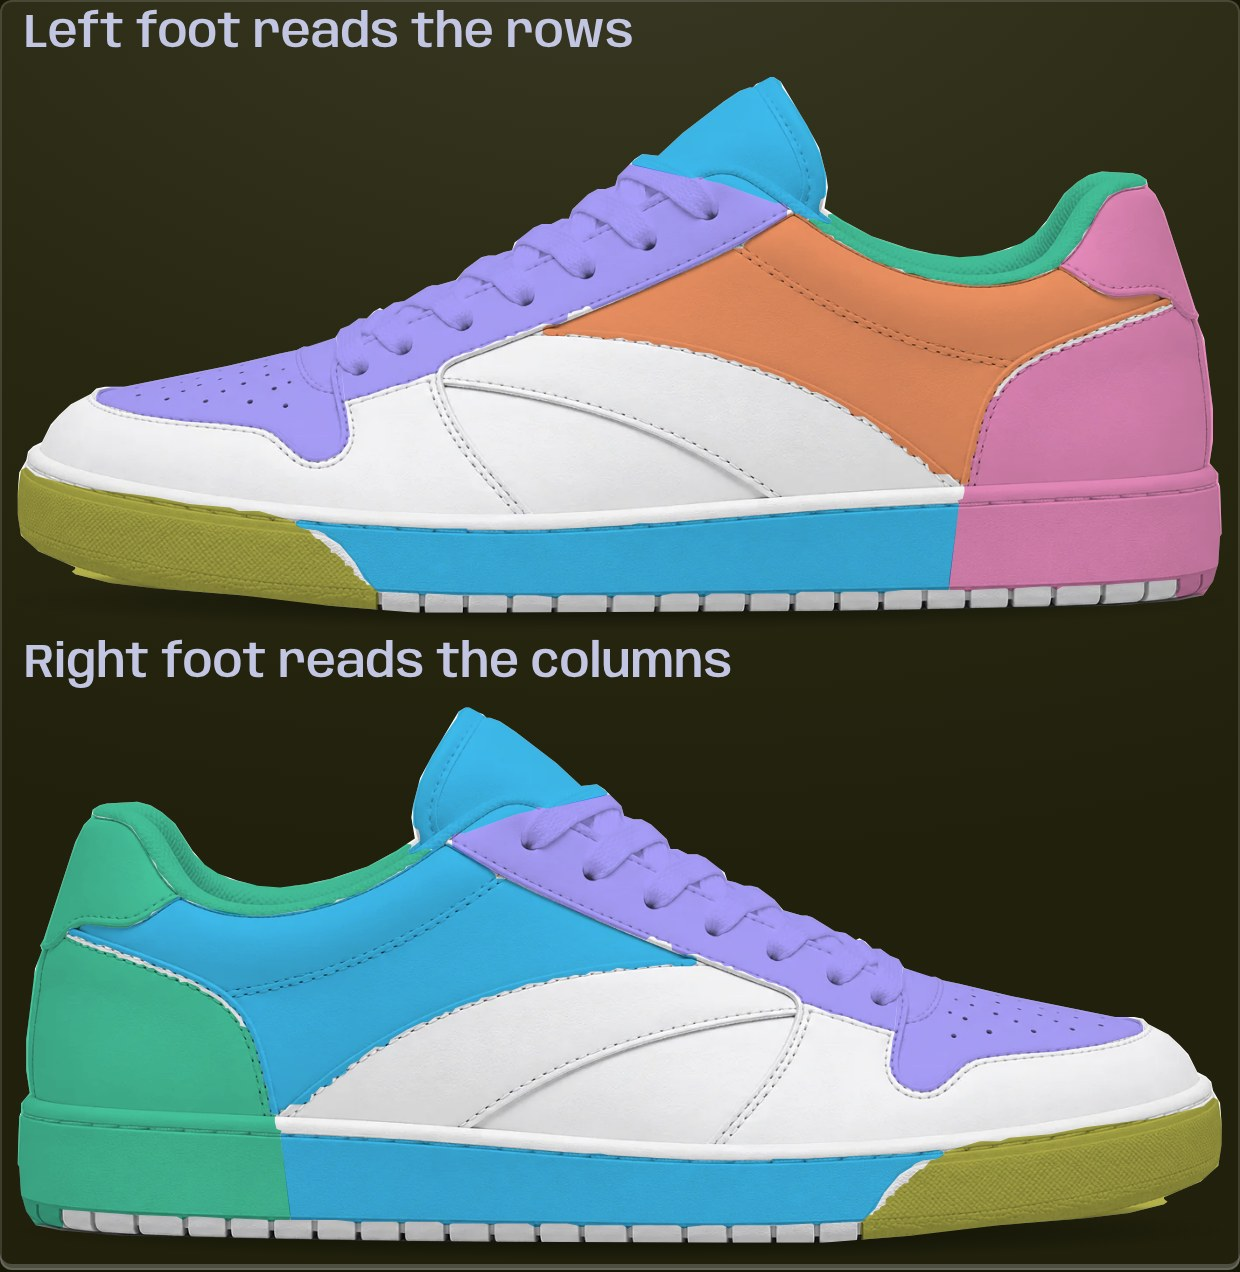
\includegraphics[width=0.62\linewidth]{figures/fig-pair.jpg}
  \caption{Pair Production for world 4{,}227{,}792. The left foot reads the grid by rows, the right foot by columns.
  The stripe, heel counter and heel sole differ, the three outlined tiles of Figure~\ref{fig:grid}.}
  \label{fig:pair}
\end{figure}

\paragraph{The workflow.} The section is a scroll story in six steps beside a pinned display case.
\begin{enumerate}
  \item \emph{Roll your world.} The visitor's world decides which panels can change between the feet. Rolling a new
        one recolors the whole site.
  \item \emph{Tune the harmony.} Turning the base hue and choosing $d$ changes every panel's pair of colors at once.
  \item \emph{Bouncer checks the print.} Anything printed on the shoe has to read on all eighteen panel colors. The
        colors are laid over a photograph of white leather with a multiply blend, so each panel is a little darker
        than its color. Bouncer multiplies each color by the measured brightness of the leather under that panel
        (between 0.78 and 0.93) before it checks, and offers the nearest passing lightness when the check fails.
  \item \emph{Paint the pair.} The visitor taps a panel to measure it. It lands on its row color on the left foot
        and its column color on the right. A button tries to force the feet to match. The six rules are listed in
        shoe terms, and a matching pair always breaks at least one of them, because at most five of six can hold.
  \item \emph{The drop.} Twelve more pairs from twelve other worlds, each following all six rules (Figure~\ref{fig:drop}).
        Choosing one makes it the visitor's world.
  \item \emph{The tag.} A hang tag records the world, the rules held and the panels that differ, with a SHA-256
        fingerprint of the design code so anyone can check a pair is the one that was made. The visitor can download
        a paint sheet with every panel's color, open the design in the Atelier, or put the pair on the Turntable.
\end{enumerate}

\begin{figure}[t]
  \centering
  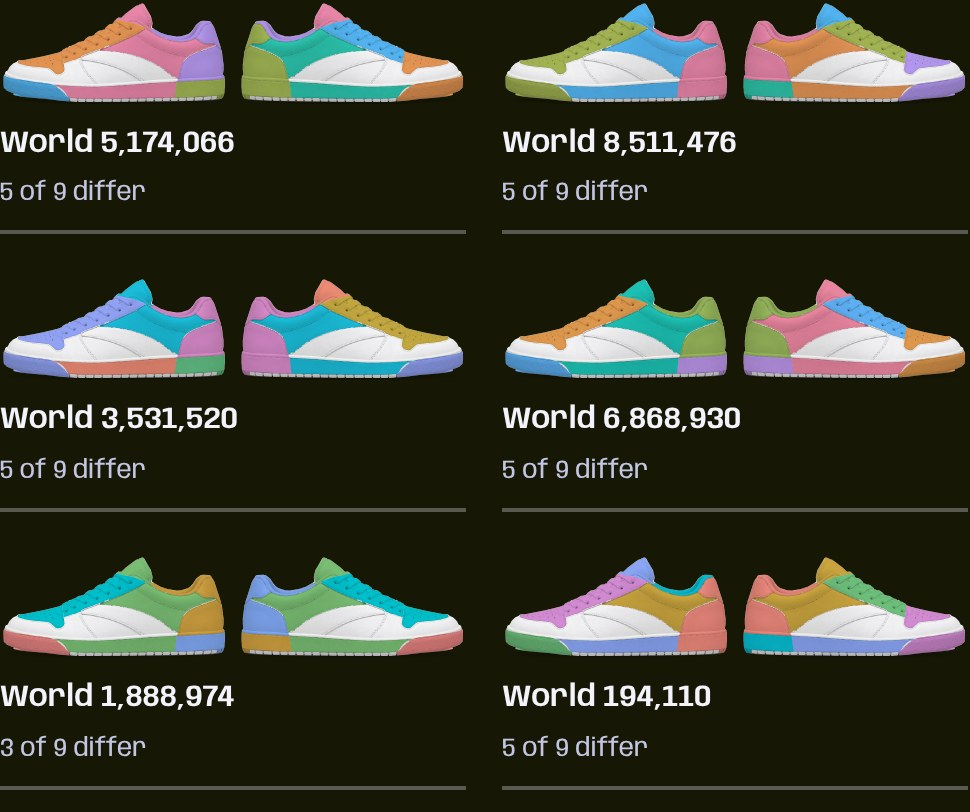
\includegraphics[width=0.62\linewidth]{figures/fig-drop.jpg}
  \caption{Six of a drop's twelve pairs, each from its own world and labeled with how many panels differ between its
  feet. Every count is odd.}
  \label{fig:drop}
\end{figure}

\paragraph{The shoe.} The shoe is a studio photograph of a plain white sneaker, made with an image generator. A script
finds the seams as thin dark lines, splits the leather into regions between them, and assigns the regions to the
nine panels, with a few hand-drawn cuts where a seam is only partly visible. Each panel becomes a vector outline. The
browser lays each panel's color over the photograph with a multiply blend, so the leather's shading, stitching and
laces show through every color. The quarter and mudguard stay white, as on a real colorway.

\paragraph{The Turntable.} The final step shows the pair in three dimensions (Figure~\ref{fig:turntable}). The model
was generated from the same photograph with an image-to-3D model (Meshy). A script fits the model's side outline to
the photograph's outline by maximizing their overlap, which reaches an intersection over union of 0.965, and stands
the model in the photograph's frame. In the browser, the nine panel outlines are painted on a flat image the size of
the photograph and projected through the shoe from the side, so a point at model position $(x,y)$ takes the color of
the photograph's pixel at the matching place. The lining and insole, found from the direction their surfaces face,
stay white. Because the 2D and 3D views share one set of outlines, they cannot disagree about which panel is which.

\begin{figure}[t]
  \centering
  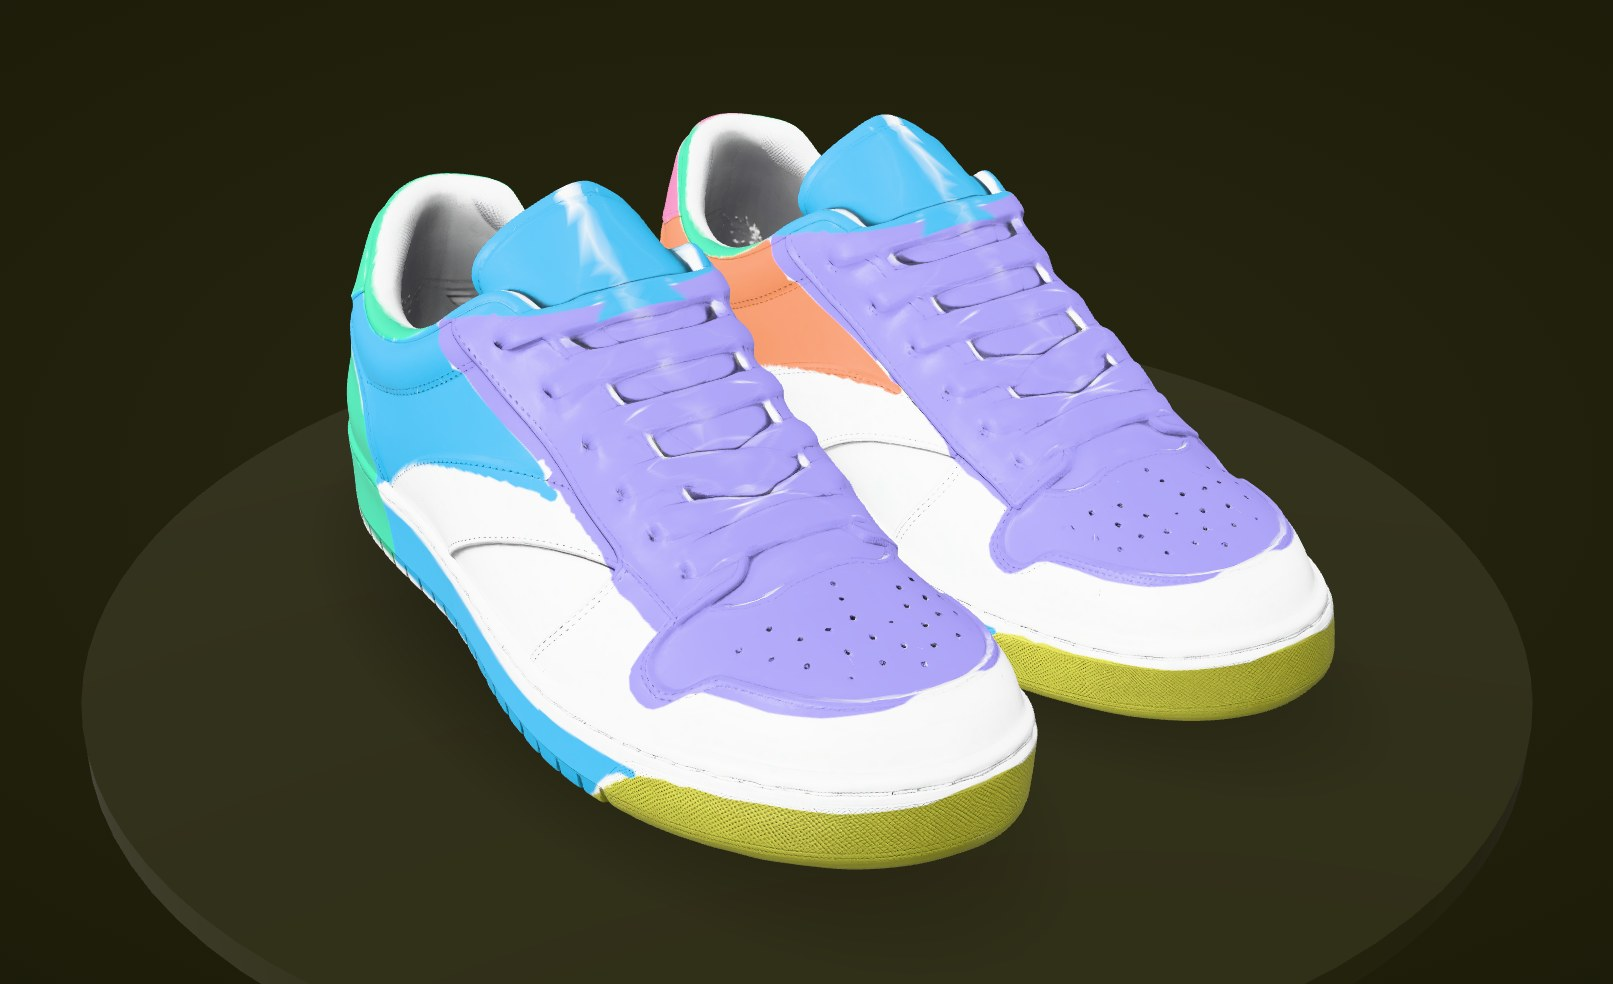
\includegraphics[width=0.72\linewidth]{figures/fig-turntable.jpg}
  \caption{The same pair on the Turntable. The panel colors are projected from the photograph's outlines onto a 3D
  model generated from the photograph. The left foot is the right foot mirrored.}
  \label{fig:turntable}
\end{figure}

\FloatBarrier
\section{Implementation and verification}
\label{sec:impl}

The engine is a set of plain JavaScript modules with no dependencies: color science, a small linear algebra library,
the quantum structures above, and exporters for CSS variables, W3C design tokens \citep{designtokens}, Tailwind and
SVG. The website, the Atelier, the runtime and the Figma plugin are built from it, and they share one convention for
turning seeds into measurements, so a world looks the same everywhere.

Every classical limit the interface shows has a test that finds it by exhaustive search (Table~\ref{tab:limits}). The
unit tests (90 at the time of writing) cover the engine and runtime. The browser tests (127) drive the website and
the Atelier in Chromium: they check, for example, that the pair's two feet differ exactly on the contextual tiles,
that forcing a match breaks a rule, that the Turntable shows the same colors as the 2D pair, and that the pages have
no accessibility violations under axe-core at phone and desktop sizes in light and dark. A separate check holds the
website to a performance budget on a throttled phone profile.

For hardware, a command line tool builds each row and column as a circuit in which every observable is measured with
its own ancilla qubit. The three values of a context are therefore measured separately, so noise can break a rule,
as it does on real devices. In the tool's noisy simulation the Mermin score is about 4.7, between the classical limit
of 4 and the ideal 6. On IBM's public devices, Dikme et al.\ measured a comparable violation using a single ancilla
per context \citep{dikme2020}. Recorded hardware shots can be saved as a pool and replayed by the website in place of
the simulator, which gives physically random worlds and a job record that serves as provenance. We do not report
new hardware results in this paper.

\section{Related work}
\label{sec:related}

\paragraph{Quantum computing and art.} Artists and researchers have used quantum computers to make music
\citep{miranda2022}, paintings \citep{crippa2024} and game content. Wootton's quantum blur encodes an image in a
quantum state and lets interference blur it \citep{wootton2020}. Quantum Brush offers painting brushes that turn strokes into
quantum algorithms and map the measured states back to color \citep{ferreira2025}. Earlier still,
WaveFunctionCollapse borrowed the language of measurement for procedural generation \citep{gumin2016}. These works use
quantum dynamics or randomness as a source of new effects. Qontext uses a different part of the theory. It takes a
no-go theorem about values and makes it a rule of the design system itself: a token is allowed, and in fact required,
to have two values, and no fixed palette can imitate it. We share Wootton's view that the useful thing at this scale is
designing software with quantum principles, not running it on quantum hardware \citep{wootton2020}.

\paragraph{Contextuality.} The theory and its experiments are reviewed by Budroni et al.\ \citep{budroni2022}. The
Mermin-Peres square has been tested with ions \citep{kirchmair2009}, on public cloud devices \citep{dikme2020} and as
a nonlocal game with photons \citep{xu2022}. Our results about differing tiles are elementary consequences of the
square. We state them because they describe what a designer sees.

\paragraph{Color and accessibility.} Qontext works in OKLCH \citep{ottosson2020,csscolor4}, where equal steps in hue
and lightness look more even than in older spaces. Contrast follows WCAG 2.2 \citep{wcag22}, with APCA \citep{apca}
reported alongside.

\section{Limits}
\label{sec:limits}

\paragraph{No quantum advantage.} Two qubits have a four-dimensional state. The browser simulates them exactly in
microseconds. A classical program that is told which context is being read can reproduce every reading, which is
exactly what our simulator does. The theorem rules out fixed tables of colors, not software. What Qontext offers is a
grammar for color with a guarantee attached: any fixed palette placed on the grid breaks at least one of the six
rules. Real hardware adds three things a simulator cannot honestly claim: physically random collapses, measured
violations of classical limits, and a job record. It adds nothing else.

\paragraph{Randomness.} Worlds on the website come from a seeded pseudorandom generator, chosen so that a world can be
shared and reproduced. They are physically random only when replayed from a hardware pool.

\paragraph{Perception.} Hue as phase is an analogy that produces even harmonies. Whether contextual palettes help
designers, or confuse readers who see a color change between two places, is an open question. We have not run a user
study. Bouncer makes sure text stays readable, but readability is not the same as clarity.

\paragraph{Contrast metrics.} The WCAG 2 ratio is known to misjudge some dark color pairs, and APCA is still a draft.
Bouncer's leather model, a single brightness factor per panel, is an approximation of a printed surface.

\paragraph{The shoe.} The panel outlines were finished by hand where seams were faint. The 3D model was generated
from one photograph, so its far side is the generator's guess. Projecting the outlines from the side is exact on the
sides of the shoe and approximate on its top, where the panel borders are the side view's borders.

\section{Conclusion}

A design token with one value is a noncontextual hidden variable. The Mermin-Peres square shows a small, precise case
where no such value exists, and we have turned that case into a working color system: tiles with two true colors, a
proof that no palette can fake them, tools that keep the results readable, and a sneaker that wears the idea on its
two feet. The physics does not make the software faster or more powerful. It gives designers a new kind of
constraint, and a reason for it that anyone can check.

\paragraph{Availability.} The website is at \url{https://qontext.qubitmen.workers.dev}. The source, including the
scripts that compute this paper's numbers and draw its figures from the engine, is at
\url{https://github.com/QubitMan-hub/Qontext}.

\bibliographystyle{unsrtnat}
\bibliography{refs}

\end{document}
